\documentclass[lang=cn,12pt]{elegantpaper}

\title{时空可组合性的编程范式}
\author{史一帆，张威，崔天翼}
\institute{北京大学，DeepSeek-AI}

\date{}

\usepackage{amsmath,amssymb,amsthm}
\usepackage{mathtools}
\usepackage{mathrsfs}
\usepackage{bm}
\usepackage{graphicx}
\usepackage{booktabs}
\usepackage{listings}
\usepackage{algorithm}
\usepackage{algpseudocode}
\usepackage{hyperref}
\usepackage{cleveref}
\usepackage{tikz}
\usetikzlibrary{automata,positioning,arrows.meta}

\addbibresource{refs.bib}

\begin{document}

\maketitle

\begin{abstract}
现代软件——从插件系统到自我演化的智能体框架——日益需要动态组合，然而其形式化基础仍不完善。我们识别出该问题的两个正交维度：时间可组合性，即在移除组件时完全撤销其副作用的能力；空间可组合性，即声明和管理组件间依赖关系并对其进行响应式管理的能力。我们通过将经典的效应（effect）与协效应（coeffect）概念提升为运行时机制来处理这两个维度。具体而言，我们形式化了可逆效应（revertible effects），其中每个上下文变换都携带一个逆变换，由运行时追踪。我们形式化了响应式协效应（reactive coeffects），其中上下文的每次变化都会根据组件的协效应规约通知该组件。我们将效应上下文和协效应上下文统一为单一上下文类型，这构成了一种编程范式。此后，我们将这些机制组合为组件的概念，并给出动态组合的演算，其元理论将时空可组合性从单个组件推广到交织组件的整个系统。我们在 Cordis 中实现了这些思想——Cordis 是一个时空可组合性的元框架，提供了具有效应追踪和协效应解析的核心库，以及具有配置协调和热模块替换的声明式组件加载器。
\end{abstract}

\section{引言}
\label{sec:1}

组合——从简单部件组装复杂系统——是软件工程的一个基本原则\cite{ref1}。传统上，组合是静态的：函数调用、模块导入和类继承在编译时解析，并在整个执行过程中保持固定。然而，现代软件日益需要动态组合，即组件在运行时被加载、卸载和重新配置。插件架构\cite{ref2}和自演化智能体框架都需要能够在运行中安全地添加和移除功能的系统，但当前实践依赖粗粒度机制\cite{ref3}，只能通过重启来重新配置，丢弃运行时状态。尽管动态组合的实际重要性日益增长，与静态组合已有的丰富形式化框架相比，其理论基础仍然不成熟。

\subsection{可组合性的维度}
\label{sec:1.1}

为了刻画动态组合的需求，我们在已被充分研究的组合代数层面之外，识别出两个正交的维度：

\begin{itemize}
\item 时间可组合性处理时间维度：在移除组件时，该组件对共享环境所做的修改必须被完全且安全地撤销。这要求追踪组件执行的每一项资源分配、事件注册和状态变更，并保证在移除时有序地回收它们。
\item 空间可组合性处理空间维度：组件必须能够以结构化且可验证的方式声明、发现和解析彼此之间的依赖关系。这要求管理依赖拓扑，并协调组件生命周期以响应依赖变化。
\end{itemize}

在静态场景中，时间可组合性归约为词法作用域（例如 RAII\cite{ref4}、括号模式\cite{ref5}），空间可组合性归约为模块导入解析\cite{ref6}。在动态场景中，组件在运行时到达和离去，两个维度都变得显著更加困难：时间可组合性必须处理作用域不受词法约束的长期有状态效应；空间可组合性必须处理在执行期间出现、消失或改变身份的依赖关系。

\subsection{动机示例}
\label{sec:1.2}

\subsubsection{插件系统}
\label{sec:1.2.1}

插件系统是动态组合的典型实例。我们以 Visual Studio Code（VSCode）——最广泛使用的可扩展 IDE 之一——作为代表性示例。

时间局限性。VSCode 在一个名为扩展宿主的共享进程中运行所有扩展。虽然扩展可以动态安装，但该宿主没有提供在运行时卸载单个扩展代码的机制。一旦扩展的 activate 函数被执行，禁用或卸载它就需要重启整个宿主，影响所有已加载的扩展。纯粹声明性的扩展（如主题、快捷键绑定和代码片段）不携带代码，可以自由移除。然而，在安装数量排名前 100 的扩展中，87 个包含可执行代码\footnote{数据于2026年6月9日从 Visual Studio Code Marketplace 获取。}，因此在移除时需要这样的重启。尽管 VSCode 提供了 deactivate 钩子，它仅作为宿主进程终止期间的优雅关闭回调，因此不支持实时移除。此外，该钩子将效应处置与效应创建（在 activate 中）分离，违反了关注点局部性，使得完整清理难以验证。

空间局限性。VSCode 确实提供了 extensionDependencies 用于声明扩展之间的依赖关系，但使用极少：在安装数量排名前 100 的扩展中，仅 7 个声明了对非内置扩展的 extensionDependencies\footnote{数据于2026年6月9日从 Visual Studio Code Marketplace 获取。}。这种稀少反映了扩展 API 的形态，它暴露固定的、表层的扩展点，如命令、视图和语言特性。扩展通过这些点向宿主贡献功能，而非彼此依赖，因此扩展间的依赖很少出现。此外，VSCode 的扩展间交互机制不提供结构化契约：它通过 vscode.extensions.getExtension(...).exports 将扩展的功能暴露给其他扩展，但返回值是无类型的（默认为 any），因此依赖方无法依赖经过检查的接口。简言之，VSCode 将扩展导向一组固定的宿主提供的扩展点，并未为它们彼此依赖提供安全、结构化的方式。

这两个局限性并非 VSCode 所独有；它们在一般插件系统中反复出现\cite{ref2,ref7}，仅在程度上有所不同。

\subsubsection{自演化智能体框架}
\label{sec:1.2.2}

现代 AI 智能体依赖运行时智能体框架\cite{ref8,ref9,ref10}。这些系统可能组合多样的工具套件\cite{ref11}和执行环境，管理权限和沙箱，维护会话状态和持久性，提供上下文管理和记忆系统\cite{ref12}，编排子智能体和多智能体工作流\cite{ref13}，并向用户和自动化暴露接口。未来的框架可能在持续服务请求的同时，生成并部署对其自身组件的修改。模型合成的可复用工具为组件级自修改提供了一个更窄的前身\cite{ref14}。每一次这样的修改本身就是动态组合的一个实例。

由于这些修改持续发生且人工监督有限或没有，动态可组合性变得不可或缺。没有时间可组合性，每次自修改都迫使完全重启，丢弃所有进程本地累积的状态；在这种频率下，累积的不可用时间变得可观，且进行中的任务被反复中断；更糟的是，一个有缺陷的自修改可能禁用恢复所需的过程本身。没有空间可组合性，每个模块必须自行检测并适应其所依赖模块在出现、消失或改变身份时的变化，且只能以临时方式实现；更糟的是，一种朴素的代码替换策略可能静默地破坏依赖方，或引入仅在重载时才显现的循环依赖。

\subsubsection{粗粒度权宜之计}
\label{sec:1.2.3}

动态可组合性受到有限形式化关注的一个原因是，操作系统和容器编排器已经提供了粗粒度的替代。操作系统以进程的粒度提供时间可组合性；容器编排器\cite{ref3}以服务的粒度提供空间可组合性。在实践中，大多数软件通过依赖这些粗粒度机制来容忍细粒度可组合性的缺失：行为异常的模块通过重启进程来处理，服务依赖由容器编排器管理。

然而，这种权宜之计带来了巨大的代价。在时间上，每次重启丢弃所有进程本地累积的状态（例如缓存、连接、部分计算），重建需要数秒到数分钟\cite{ref15}；在此期间维持可用性需要冗余副本，产生资源开销以补偿无法恢复单个组件的缺陷。在空间上，容器级编排无法表达共享地址空间的组件之间的依赖关系，并为本可以是本地函数调用的交互引入了网络开销。两种机制都在进程和容器的边界上运作，但现代系统日益在更细的层面上进行组合。这种粒度失配需要一种组合抽象，在与组件自身相同的层面上管理效应和依赖。

\subsection{贡献}
\label{sec:1.3}

动态可组合性的两个维度分别关注计算如何修改其环境以及如何依赖于其环境。这两个方向正是效应系统\cite{ref16,ref17}和协效应系统\cite{ref18,ref19}所形式化的内容：效应提供了关于环境修改推理的形式化词汇，协效应则提供了关于环境需求推理的形式化词汇。然而，现有的形式化将推理限制在词法固定作用域上的编译时分析，并未扩展到组件在运行时到达和离去的动态场景。通过将效应提升为可逆的运行时模型、将协效应提升为反应式依赖解析机制，我们获得了动态可组合性的统一形式化基础，该基础与语言无关，适用于任何需要动态组合的软件架构。我们做出以下贡献：

\begin{enumerate}
\item 我们形式化了可逆效应（\S\ref{subsec:3.1}）：每个上下文变换携带一个运行时追踪的显式逆操作，且追踪和恢复均保持组合性，因此在组件移除时上下文得以恢复。这建立了局部时间可组合性。
\item 我们形式化了反应式协效应（\S\ref{subsec:3.2}）：组件将其所需的协效应声明为规约，上下文的每次变更根据该规约通知组件为激活、去激活或中性的。这建立了局部空间可组合性。
\item 我们将效应上下文和协效应上下文统一为单一的上下文类型（\S\ref{subsec:3.3}），其中协效应上的观察等价性为效应提供了独立性，构成了时空可组合性的编程范式。
\item 我们给出了动态组合的演算（\S\ref{sec:4}），将两种机制组合为组件的概念，并为其生命周期配备了操作语义。其元理论将时空可组合性从单个组件推广到交织组件的整个系统。
\item 我们在 Cordis（\S\ref{sec:5}）中实现了这些思想，这是一个时空可组合性的元框架，提供了实现形式化模型的核心库（包含效应追踪和协效应解析），以及具有配置调和和热模块替换的声明式组件加载器。
\end{enumerate}

\section{预备知识}
\label{sec:2}

本节提供效应与协效应系统的简要概述——这是支撑我们工作的两个理论支柱。我们假设读者熟悉基本的类型论和范畴论；此处的目标是确定记号并引入第 \S\ref{sec:3} 节将作为运行时机制加以实现的关键抽象。

\subsection{效应}
\label{sec:2.1}

在简单类型 $\lambda$ 演算 (STLC) \cite{ref20, ref21} 中，类型推导 $\Gamma \vdash t : T$ 表明项 $t$ 在上下文 $\Gamma$ 下具有类型 $T$。效应系统对类型加以精化，以描述计算可能产生哪些副作用，从而得到如下形式的推导
\begin{equation}
\label{eq:2.1}
\Gamma \vdash t : T \mid \textit{effect}
\end{equation}
此处，结果类型附带效应代数的一个元素作为标注，该元素描述了计算可能产生哪些副作用，从而使得对有状态计算的组合推理成为可能。这一方法源自 Lucassen 和 Gifford \cite{ref22}，他们引入了一种区分类型、效应和区域的类别化类型系统，以发现并行程序中的调度约束。

\subsubsection{单子效应}
\label{sec:2.1.1}

Moggi \cite{ref16} 首次通过单子对计算效应进行范畴论建模；Wadler \cite{ref23} 在 Haskell 中推广了该方法。范畴 $\mathcal{C}$ 上的单子 $(T, \eta, \mu)$ 将效应计算封装为 $T(A)$ 类型的值，其中 $\eta : A \to T(A)$ 将纯值提升，$\mu : T(T(A)) \to T(A)$ 将嵌套计算顺序组合。经典实例包括 Maybe 单子（用于部分性）、State 单子（用于可变状态）和 IO 单子（用于外部交互）。

\subsubsection{代数效应}
\label{sec:2.1.2}

Plotkin 和 Power \cite{ref17, ref24} 证明了代数运算确定单子，建立了一个效应接口与其实现解耦的框架。效应签名 $\Sigma$ 声明一组运算（例如，用于状态的 $\mathrm{get} : () \to S$、$\mathrm{put} : S \to ()$）；程序自由地调用运算，而无需绑定到特定的解释。Plotkin 和 Pretnar \cite{ref25} 随后引入了效应处理器，通过提供续延语义来解释运算：
\begin{equation}
\label{eq:2.2}
\mathrm{handle}\ e\ \mathrm{with}\ \{ \mathrm{op}(v, \kappa) \mapsto \ldots \}
\end{equation}
处理器接收运算参数 $v$ 和定界续延 $\kappa$，它可以调用零次、一次或多次，从而在统一框架内实现异常、协程和非确定性 \cite{ref26}。诸如 Koka \cite{ref27, ref28}、Eff \cite{ref29} 和 OCaml 5 \cite{ref30} 等语言已在不同设计权衡下采用了代数效应。

\subsection{协效应}
\label{sec:2.2}

与效应对偶地，协效应系统 \cite{ref18, ref31} 丰富的是上下文而非类型，从而得到如下形式的推导
\begin{equation}
\label{eq:2.3}
\Gamma \mid \textit{coeffect} \vdash t : T
\end{equation}
此处，上下文附带协效应代数的一个元素作为标注，描述计算从其环境中需要什么，例如要访问的资源、要持有的权限或要依赖的服务。效应建模的是程序对世界的影响，而协效应建模的是世界对程序的约束。

\subsubsection{余单子协效应}
\label{sec:2.2.1}

使用余单子来构造上下文依赖计算的思想首先由 Uustalu 和 Vene \cite{ref32} 发展，他们提出了对称（半）单子余单子作为 Moggi 效应单子框架的对偶，捕获了数据流和属性求值等概念。Petricek 等人 \cite{ref18} 在此基础上提出了协效应，作为上下文依赖性的统一静态分析。余单子 $(D, \varepsilon, \delta)$ 捕获上下文依赖计算：$\varepsilon : D(A) \to A$ 从上下文中提取当前值，$\delta : D(A) \to D(D(A))$ 复制上下文以供嵌套访问。环境余单子 $D(X) = E \times X$ 建模对固定环境 $E$ 的依赖；流余单子 $D(X) = \mathbb{N} \to X$ 建模对时序数据的依赖。

\subsubsection{分次协效应}
\label{sec:2.2.2}

为实现更细粒度的追踪，分次协效应系统使用预序半环 $\mathcal{S} = (S, \leqslant, +, \times, 0, 1)$ 作为协效应代数 \cite{ref33}，这一方法后来由 Gaboardi 等人 \cite{ref19} 与分次效应统一。$S$ 的元素标注每个变量绑定以量化其使用：0 表示未使用，1 表示线性使用，$n$ 表示有界使用，$\infty$ 表示无限制使用。半环运算分别按顺序（$\times$）和并行（$+$）组合协效应，从而在统一的代数框架 \cite{ref37} 内实现精确的资源追踪、灵敏度分析 \cite{ref34} 和信息流控制 \cite{ref35, ref36}。

\subsection{与动态可组合性的关系}
\label{sec:2.3}

效应与协效应系统沿两个互补方向组织关于计算的推理：效应描述计算如何修改其环境，而协效应描述计算如何依赖其环境。这两个方向对应于第 \S\ref{sec:1} 中所识别的动态可组合性的两个维度：
\begin{itemize}
\item 时间可组合性要求组件对共享环境的修改在卸载时可逆。相关的效应是有状态的效应，它们持久地变换该环境；撤销这种变换要求它具有逆。
\item 空间可组合性要求组件间依赖被声明并响应式地管理。此类依赖正是协效应所捕获的内容，管理它们就是将每个依赖与环境的供给进行匹配。
\end{itemize}

然而，经典的效应与协效应系统是静态工具：效应在词法固定的作用域内被追踪，并由编译时处理器处置；协效应标注依据执行前确定的上下文进行验证。相比之下，动态组合要求这些保证对在运行时到达和离开的组件成立，且所面对的上下文持续演化。任何固定的词法作用域都无法界定部署后加载的插件；任何编译时上下文都无法预见运行时配置所产生的依赖。

这促成了视角的转变：我们不是用更多标注来扩展静态类型系统，而是将效应与协效应的概念结构具体化，使得运行时可以直接对其进行操作，从而动态地建立这些系统在静态时所提供的保证。
\section{可逆效应与响应式协效应}\label{sec:3}

本节将第\S\ref{sec:2}中引入的效应与协效应概念提升为运行时机制，构建动态组合的理论。核心思想是将承载效应与协效应的定型上下文转化为上下文类型，即把上下文具体化为一等实体的运行时可操作类型。对于效应类型，我们将其建模为附带逆元的上下文变换，实现局部的时间可组合性。对于协效应上下文，我们将其建模为承载依赖信息的类型，实现局部的空间可组合性。协效应上的观测等价随后为效应提供独立性。承载效应与协效应的统一上下文本身构成了一种编程范式。

\subsection{可逆效应}\label{subsec:3.1}

时间可组合性是在运行时加载和卸载组件，使得卸载时共享环境恢复到组合前状态的能力。这要求组件对环境的每一次修改既是可追踪的，又是可恢复的。因此，我们将效应建模为$\Gamma \to \Gamma \times (\Gamma \to \Gamma)$类型的函数：施加于当前上下文，它产生修改后的上下文连同显式的逆元。提供该逆元使效应可被逆转，将其返回运行时使效应可被追踪。我们称此类效应为可逆的：通过在执行期间追踪和组合这些逆元，完全的环境恢复成为一种结构性保证。

\subsubsection{效应上下文}\label{subsubsec:3.1.1}

给定任何非纯函数$f_{\mathrm{impure}}: X \to Y$，我们将其转化为纯形式$f: \Gamma \times X \to \Gamma \times Y$，其中$\Gamma$是上下文，所有可能的副作用可以表示为$\Gamma$上的变换。对于任何固定输入$x: X$，诱导映射$\gamma \mapsto \mathrm{pr}_1(f(\gamma, x))$独立于返回值地捕获了$f$的副作用。因此$\Gamma$上的效应存在于变换$\Gamma \to \Gamma$在复合$\circ$下的幺半群中，其中每个幺半群公理都有作为效应性质的直接解读：
\begin{itemize}
\item 封闭性：两个效应的顺序复合仍是效应；
\item 结合律：复合效应与括号方式无关；
\item 单位元：$\mathrm{id}_\Gamma$，$\Gamma$上的恒等函数，作为复合的单位元。
\end{itemize}

为了建模可撤销的效应，我们将每个变换$f$与另一个撤销$f$的变换$g$配对，并称$g$为$f$的左逆，全文简称为逆元。撤销是单向的：逆元所满足的是$g \circ f$而非$f \circ g$。变换对具有自身的乘法：

\begin{definition}\label{def:3.1}
定义上下文变换对的扭曲复合为
\begin{equation}\label{eq:3.4}
(f_1, g_1) \circ (f_2, g_2) \coloneqq (f_1 \circ f_2, g_2 \circ g_1)
\end{equation}
\end{definition}

与$\circ$本身一样，左操作数在右操作数之后作用，逆元以相反顺序累积。这使$(\Gamma \to \Gamma) \times (\Gamma \to \Gamma)$成为以$(\mathrm{id}_\Gamma, \mathrm{id}_\Gamma)$为单位元的幺半群，即变换幺半群与其对偶的积，我们称之为$\Gamma$上的扭曲复合幺半群$\mathfrak{T}_\Gamma$。

为了在上下文本身中追踪效应，我们引入以下定义：

\begin{definition}\label{def:3.2}
给定上下文$\Gamma$，定义其效应上下文为：
\begin{equation}\label{eq:3.5}
\partial\Gamma \coloneqq \Gamma \times (\Gamma \to \Gamma)
\end{equation}
\end{definition}

它可以理解为一个对$(\gamma, \varphi)$，其中：
\begin{itemize}
\item $\gamma: \Gamma$是当前上下文状态；
\item $\varphi: \Gamma \to \Gamma$是累积器，即迄今为止所执行效应的逆元的复合，也是将上下文恢复到初始状态的函数。
\end{itemize}

特别地，初始效应上下文可以表示为$(\gamma_0, \mathrm{id}_\Gamma)$。

我们也记$\partial^2\Gamma = \partial\Gamma \times (\partial\Gamma \to \partial\Gamma)$，以此类推形成塔。

鉴于累积器$\varphi$的存在，对$\partial\Gamma$执行的所有效应都可以被追踪和恢复。我们现在给出追踪和恢复的具体构造。

\begin{definition}\label{def:3.3}
定义上下文函数对上的变换$\mathrm{track}_\Gamma$：
\begin{equation}\label{eq:3.6}
\mathrm{track}_\Gamma : (\Gamma \to \Gamma) \times (\Gamma \to \Gamma) \to \partial\Gamma \to \partial\Gamma
\end{equation}
\[
\mathrm{track}_\Gamma = (f, g) \mapsto (\gamma, \varphi) \mapsto (f(\gamma), \varphi \circ g)
\]
\end{definition}

该变换将前向函数$f$连同候选逆元$g$转化为效应上下文$\partial\Gamma$的变换。将$\mathrm{track}_\Gamma(f, g)$施加于状态$(\gamma, \varphi)$，通过$f$变换$\gamma$并将逆元$g$复合到$\varphi$上，从而在上下文中追踪$f$的效应。

\begin{theorem}\label{thm:3.4}
对于每个$(f, g) \in (\Gamma \to \Gamma) \times (\Gamma \to \Gamma)$，以下图表交换，即
\begin{equation}\label{eq:3.7}
\mathrm{pr}_1 \circ \mathrm{track}_\Gamma(f, g) = f \circ \mathrm{pr}_1
\end{equation}
\end{theorem}

\begin{proof}
对于所有$(\gamma, \varphi) \in \partial\Gamma$：
\[
(\mathrm{pr}_1 \circ \mathrm{track}_\Gamma(f, g))(\gamma, \varphi) = \mathrm{pr}_1(f(\gamma), \varphi \circ g) = f(\gamma) = (f \circ \mathrm{pr}_1)(\gamma, \varphi)
\]
\end{proof}

\begin{theorem}\label{thm:3.5}
$\mathrm{track}_\Gamma$是从$\mathfrak{T}_\Gamma$到$\partial\Gamma \to \partial\Gamma$的幺半群同态。即，
\begin{enumerate}
\item $\mathrm{track}_\Gamma(\mathrm{id}_\Gamma, \mathrm{id}_\Gamma) = \mathrm{id}_{\partial\Gamma}$；
\item 对于所有$(f_1, g_1), (f_2, g_2) \in \mathfrak{T}_\Gamma$，
\begin{equation}\label{eq:3.8}
\mathrm{track}_\Gamma((f_1, g_1) \circ (f_2, g_2)) = \mathrm{track}_\Gamma(f_1, g_1) \circ \mathrm{track}_\Gamma(f_2, g_2)
\end{equation}
\end{enumerate}
\end{theorem}

\begin{proof}
\begin{enumerate}
\item 单位元映为单位元，因为$\mathrm{track}_\Gamma(\mathrm{id}_\Gamma, \mathrm{id}_\Gamma)(\gamma, \varphi) = (\gamma, \varphi \circ \mathrm{id}_\Gamma) = (\gamma, \varphi)$。
\item 对于乘法，取任意$(\gamma, \varphi) \in \partial\Gamma$：
\[
(\mathrm{track}_\Gamma(f_1, g_1) \circ \mathrm{track}_\Gamma(f_2, g_2))(\gamma, \varphi) = \mathrm{track}_\Gamma(f_1, g_1)(f_2(\gamma), \varphi \circ g_2)
\]
\[
= (f_1(f_2(\gamma)), \varphi \circ g_2 \circ g_1) = \mathrm{track}_\Gamma(f_1 \circ f_2, g_2 \circ g_1)(\gamma, \varphi)
\]
\end{enumerate}
\end{proof}

\begin{definition}\label{def:3.6}
定义$\partial\Gamma$上的变换$\mathrm{recover}_\Gamma$：
\begin{equation}\label{eq:3.9}
\mathrm{recover}_\Gamma : \partial\Gamma \to \partial\Gamma
\end{equation}
\[
\mathrm{recover}_\Gamma = (\gamma, \varphi) \mapsto (\varphi(\gamma), \mathrm{id}_\Gamma)
\]
\end{definition}

该变换将恢复函数$\varphi$施加于当前状态$\gamma$，并将$\varphi$重置为单位元。下图说明了一组效应$\mathrm{track}(f_1, g_1), \cdots, \mathrm{track}(f_n, g_n)$施加于$\partial\Gamma$后，$\mathrm{recover}$如何将上下文恢复到初始状态：

追踪效应后再执行恢复将初始效应上下文带回自身。每个追踪步骤所保留的是恢复本身的结果，无论从哪个状态执行：

\begin{theorem}\label{thm:3.7}
对于每个$(\gamma, \varphi) \in \partial\Gamma$和每个满足$g(f(\gamma)) = \gamma$的对$(f, g)$，
\begin{equation}\label{eq:3.10}
\mathrm{recover}_\Gamma(\mathrm{track}_\Gamma(f, g)(\gamma, \varphi)) = \mathrm{recover}_\Gamma(\gamma, \varphi)
\end{equation}
\end{theorem}

\begin{proof}
\begin{align*}
\mathrm{recover}_\Gamma(\mathrm{track}_\Gamma(f, g)(\gamma, \varphi)) &= \mathrm{recover}_\Gamma(f(\gamma), \varphi \circ g) \\
&= (\varphi(g(f(\gamma))), \mathrm{id}_\Gamma) \\
&= (\varphi(\gamma), \mathrm{id}_\Gamma) = \mathrm{recover}_\Gamma(\gamma, \varphi)
\end{align*}
\end{proof}

一组对不需要单独论证。设$(f_1, g_1), \cdots, (f_n, g_n)$从$(\gamma, \varphi)$依次施加，记$\delta_0 = \gamma$和$\delta_i = f_i(\delta_{i-1})$。由定理\ref{thm:3.5}，复合$\mathrm{track}_\Gamma(f_n, g_n) \circ \cdots \circ \mathrm{track}_\Gamma(f_1, g_1)$是扭曲复合$(f_n \circ \cdots \circ f_1, g_1 \circ \cdots \circ g_n)$的$\mathrm{track}_\Gamma$，若对每个$i$有$g_i(\delta_i) = \delta_{i-1}$，则$(g_1 \circ \cdots \circ g_n)(\delta_n) = \delta_0 = \gamma$。因此该对在$\gamma$处满足定理\ref{thm:3.7}的假设，应用一次定理得到
\begin{equation}\label{eq:3.11}
\mathrm{recover}_\Gamma((\mathrm{track}_\Gamma(f_n, g_n) \circ \cdots \circ \mathrm{track}_\Gamma(f_1, g_1))(\gamma, \varphi)) = \mathrm{recover}_\Gamma(\gamma, \varphi)
\end{equation}

取$(\gamma, \varphi) = (\gamma_0, \mathrm{id}_\Gamma)$，恢复将以此方式到达的每个状态带回$(\gamma_0, \mathrm{id}_\Gamma)$。满足$g \circ f = \mathrm{id}_\Gamma$的对在每个状态都满足假设。

恢复通过量$\varphi(\gamma)$读取状态，我们将$\varphi(\gamma) = \gamma_0$称为$\partial\Gamma$中状态的健康性不变式。

\subsubsection{可逆效应函数}\label{subsubsec:3.1.2}

前一节的追踪/恢复模型将逆元视为先验给定的：$\mathrm{track}_\Gamma(f, g)$在任何上下文状态出现之前就固定了$g$，因此一个$g$必须服务于效应被施加的每个状态。然而在实践中，每个效应的逆元并非先验已知的：它必须由调用者在效应施加点提供。此外，恢复是全有或全无的：它不能选择性地撤销一个效应而保留其他效应。为解决这两个问题，我们在输入和输出两侧分别增强模型：
\begin{enumerate}
\item 在输入侧，我们不仅变换$\Gamma$，还同时返回逆元函数，使逆元在效应施加处提供：$\Gamma \to \Gamma \times (\Gamma \to \Gamma)$，即$\Gamma \to \partial\Gamma$；
\item 在输出侧，我们不仅变换$\partial\Gamma$，还同时返回逆元函数，使一个效应可被撤销而其他效应得以保留：$\partial\Gamma \to \partial\Gamma \times (\partial\Gamma \to \partial\Gamma)$，即$\partial\Gamma \to \partial^2\Gamma$。
\end{enumerate}

这种增强保持了输入与输出之间的结构一致性，因此我们仍然可以定义相应的理论来维护$\mathrm{track}$的数学性质。所得类型是效应函数$\mathfrak{E}_\Gamma$及其见证细化$\mathfrak{E}^*_\Gamma$：

\begin{definition}\label{def:3.8}
定义效应函数$\mathfrak{E}_\Gamma$和见证效应函数$\mathfrak{E}^*_\Gamma$为：
\begin{equation}\label{eq:3.12}
\mathfrak{E}_\Gamma \coloneqq \Gamma \to \Gamma \times (\Gamma \to \Gamma)
\end{equation}
\[
\mathfrak{E}^*_\Gamma \coloneqq (e: \Gamma \to \Gamma \times (\Gamma \to \Gamma)) \times ((\gamma: \Gamma) \to ((\delta: \Gamma) \times (g: \Gamma \to \Gamma) \times ((\delta, g) = e(\gamma) \to g(\delta) = \gamma)))
\]
\end{definition}

其中$e(\gamma)$产生一个对$(\delta, g)$，表示：
\begin{itemize}
\item $\delta: \Gamma$是新上下文；
\item $g: \Gamma \to \Gamma$是当前效应的逆元函数。
\end{itemize}

$\mathfrak{E}^*_\Gamma$的一个元素按状态选择其逆元，约束$g(\delta) = \gamma$将选择限制在逆转效应施加处的效果上，而$g$在其他任何地方不受约束。满足$g \circ f = \mathrm{id}_\Gamma$的单个$g$在每个状态同时满足约束，并通过$(f, g) \mapsto \gamma \mapsto (f(\gamma), g)$诱导$\mathfrak{E}^*_\Gamma$的一个元素，定理\ref{thm:3.11}表明这是一个同态。约束可以可视化为以下交换图，确保逆元$e$返回确实逆转了$e$被施加处的变换：

由于效应函数$\mathfrak{E}_\Gamma$不再是上下文上的自同态，它们不能直接复合。因此我们定义效应复合的新运算：

\begin{definition}\label{def:3.9}
给定函数$f, g \in \mathfrak{E}_\Gamma$，定义其效应复合$f \diamond g$为：
\begin{equation}\label{eq:3.13}
f \diamond g : \Gamma \to \partial\Gamma
\end{equation}
\[
f \diamond g = \gamma \mapsto \mathbf{let}\;(\delta, s) = g(\gamma)\;\mathbf{in}\;\mathbf{let}\;(\varepsilon, t) = f(\delta)\;\mathbf{in}\;(\varepsilon, s \circ t)
\]
\end{definition}

\begin{theorem}\label{thm:3.10}
效应复合将$\mathfrak{T}_\Gamma$的幺半群结构转移到$\mathfrak{E}_\Gamma$。即，
\begin{enumerate}
\item $(\mathfrak{E}_\Gamma, \diamond)$是以$\eta_\Gamma \coloneqq \gamma \mapsto (\gamma, \mathrm{id}_\Gamma)$为单位元的幺半群；
\item 映射$(f, g) \mapsto \gamma \mapsto (f(\gamma), g)$是从$\mathfrak{T}_\Gamma$到$\mathfrak{E}_\Gamma$的幺半群同态。
\end{enumerate}
\end{theorem}

\begin{proof}
\begin{enumerate}
\item 结合律和单位元律由$\circ$的相应定律逐分量得到。
\item 记$e_i = \gamma \mapsto (f_i(\gamma), g_i)$；则$(e_1 \diamond e_2)(\gamma) = (f_1(f_2(\gamma)), g_2 \circ g_1)$，即$(f_1, g_1) \circ (f_2, g_2)$的像，而$(\mathrm{id}_\Gamma, \mathrm{id}_\Gamma)$映射到$\eta_\Gamma$。
\end{enumerate}
\end{proof}

\begin{theorem}\label{thm:3.11}
见证性在效应复合下保持，一致逆元在每个状态见证。即，
\begin{enumerate}
\item $\mathfrak{E}^*_\Gamma$是$\mathfrak{E}_\Gamma$的子幺半群；
\item 定理\ref{thm:3.10}的同态将每个满足$g \circ f = \mathrm{id}_\Gamma$的对带入$\mathfrak{E}^*_\Gamma$。
\end{enumerate}
\end{theorem}

\begin{proof}
\begin{enumerate}
\item 由于$\mathrm{id}_\Gamma(\gamma) = \gamma$，单位元属于$\mathfrak{E}^*_\Gamma$。对于封闭性，取$f, g \in \mathfrak{E}^*_\Gamma$和任意$\gamma \in \Gamma$，令$(\delta, s) = g(\gamma)$，$(\varepsilon, t) = f(\delta)$，使得$(f \diamond g)(\gamma) = (\varepsilon, s \circ t)$。则$s(\delta) = \gamma$且$t(\varepsilon) = \delta$，因此$(s \circ t)(\varepsilon) = s(\delta) = \gamma$。
\item $g \circ f = \mathrm{id}_\Gamma$在每个$\gamma$给出$g(f(\gamma)) = \gamma$，因此这样一对的像在每个状态都被见证。
\end{enumerate}
\end{proof}

正如$\mathrm{track}$将$\Gamma$上的变换对提升到$\partial\Gamma$，我们定义$\mathrm{effect}$将$\mathfrak{E}_\Gamma$提升到$\mathfrak{E}_{\partial\Gamma}$：

\begin{definition}\label{def:3.12}
定义效应函数变换$\mathrm{effect}_\Gamma$为：
\begin{equation}\label{eq:3.14}
\mathrm{effect}_\Gamma : \mathfrak{E}_\Gamma \to \partial\Gamma \to \partial^2\Gamma
\end{equation}
\[
\mathrm{effect}_\Gamma = e \mapsto (\gamma, \varphi) \mapsto \mathbf{let}\;(\delta, g) = e(\gamma)\;\mathbf{in}\;((\delta, \varphi \circ g), \mathrm{track}_\Gamma(g, \mathrm{pr}_1 \circ e))
\]
\end{definition}

由于$\mathrm{effect}_\Gamma(e)$本身属于$\mathfrak{E}_{\partial\Gamma}$，它返回的逆元是定义\ref{def:3.8}在更高一层意义上的逆元。该逆元本身是交换效应两个方向所得对的追踪。普通追踪规则再次适用：撤销效应本身也是一种效应，通过$g$变换状态，而撤销它的方法是再次执行该效应，这正是$\mathrm{pr}_1 \circ e$所做的。因此逆元复合到它所接收的累积器上，完全如$\mathrm{track}$所规定。

我们现在可以证明$\mathrm{effect}$与$\mathrm{track}$类似的性质。

\begin{theorem}\label{thm:3.13}
$\mathrm{effect}$保持$\diamond$运算。即，$\forall f, g \in \mathfrak{E}_\Gamma$：
\begin{equation}\label{eq:3.15}
\mathrm{effect}_\Gamma(f) \diamond \mathrm{effect}_\Gamma(g) = \mathrm{effect}_\Gamma(f \diamond g)
\end{equation}
\end{theorem}

\begin{proof}
取任意$(\gamma, \varphi) \in \partial\Gamma$，令$(\delta, s) = g(\gamma)$和$(\varepsilon, t) = f(\delta)$，使得$(f \diamond g)(\gamma) = (\varepsilon, s \circ t)$且$\mathrm{pr}_1 \circ (f \diamond g) = (\mathrm{pr}_1 \circ f) \circ (\mathrm{pr}_1 \circ g)$。则
\begin{align*}
&(\mathrm{effect}_\Gamma(f) \diamond \mathrm{effect}_\Gamma(g))(\gamma, \varphi) \\
&= ((\varepsilon, \varphi \circ s \circ t), \mathrm{track}_\Gamma(s, \mathrm{pr}_1 \circ g) \circ \mathrm{track}_\Gamma(t, \mathrm{pr}_1 \circ f)) \\
&= ((\varepsilon, \varphi \circ s \circ t), \mathrm{track}_\Gamma(s \circ t, (\mathrm{pr}_1 \circ f) \circ (\mathrm{pr}_1 \circ g))) \\
&= \mathrm{effect}_\Gamma(f \diamond g)(\gamma, \varphi)
\end{align*}
其中第一步在$(\gamma, \varphi)$和$(\delta, \varphi \circ s)$处展开定义\ref{def:3.12}，第二步由定理\ref{thm:3.5}得到，第三步折叠定义\ref{def:3.12}。
\end{proof}

两个层次之间的关系如下图所示。其上三角是$e$的见证条件，根据定义\ref{def:3.8}，其下三角是$e'$是否像$e$一样被见证的问题。

在层次之间，投射$\mathrm{pr}_1$将每个提升的映射与其所提升的映射相关联，正如定理\ref{thm:3.4}中对$\mathrm{track}_\Gamma$所做的那样。

\begin{theorem}\label{thm:3.14}
设$e \in \mathfrak{E}_\Gamma$，记$f \coloneqq \mathrm{pr}_1 \circ e$，并令$e' \coloneqq \mathrm{effect}_\Gamma(e)$，其前向映射为$f' \coloneqq \mathrm{pr}_1 \circ e'$。则
\begin{enumerate}
\item $\mathrm{pr}_1 \circ f' = f \circ \mathrm{pr}_1$；
\item 对于每个$(\gamma, \varphi) \in \partial\Gamma$，提升逆元$g' \coloneqq \mathrm{pr}_2(e'(\gamma, \varphi))$和在该处见证的逆元$g \coloneqq \mathrm{pr}_2(e(\gamma))$满足$\mathrm{pr}_1 \circ g' = g \circ \mathrm{pr}_1$。
\end{enumerate}
\end{theorem}

\begin{proof}
\begin{enumerate}
\item 由定义\ref{def:3.12}，$f'(\gamma, \varphi) = (f(\gamma), \varphi \circ g)$，其状态为$f(\gamma) = (f \circ \mathrm{pr}_1)(\gamma, \varphi)$。
\item 这是对$g' = \mathrm{track}_\Gamma(g, f)$应用定理\ref{thm:3.4}。
\end{enumerate}
\end{proof}

下三角是否闭合可以通过计算提升逆元的返回值来确定：

\begin{theorem}\label{thm:3.15}
设$e \in \mathfrak{E}^*_\Gamma$并记$f \coloneqq \mathrm{pr}_1 \circ e$。固定$(\gamma, \varphi) \in \partial\Gamma$，令$(\delta, g) = e(\gamma)$，并记$(\Delta, g')$为$\mathrm{effect}_\Gamma(e)$在$(\gamma, \varphi)$处的值。则
\begin{equation}\label{eq:3.16}
g'(\Delta) = (\gamma, \varphi \circ g \circ f)
\end{equation}
\end{theorem}

状态被精确恢复。累积器也被恢复，等价于$\mathrm{effect}_\Gamma(e) \in \mathfrak{E}^*_{\partial\Gamma}$，当且仅当$g \circ f = \mathrm{id}_\Gamma$；在任何情况下$(\varphi \circ g \circ f)(\gamma) = \varphi(\gamma)$，因此健康性不变式得以保持。

\begin{proof}
由定义\ref{def:3.12}，$\Delta = (\delta, \varphi \circ g)$且$g' = \mathrm{track}_\Gamma(g, f)$，所以
\[
g'(\Delta) = (g(\delta), \varphi \circ g \circ f) = (\gamma, \varphi \circ g \circ f)
\]
其中使用了$g(\delta) = \gamma$。属于$\mathfrak{E}^*_{\partial\Gamma}$要求在每个输入处等于$(\gamma, \varphi)$；取$\varphi = \mathrm{id}_\Gamma$将累积器的等式变为$g \circ f = \mathrm{id}_\Gamma$，而该条件反过来对每个$\varphi$给出累积器的等式。最后$(\varphi \circ g \circ f)(\gamma) = \varphi(g(\delta)) = \varphi(\gamma)$。
\end{proof}

因此下三角仅在$\gamma$处见证的逆元在每个状态逆转$f$时才闭合，因此$\mathrm{effect}_\Gamma$不将$\mathfrak{E}^*_\Gamma$带入$\mathfrak{E}^*_{\partial\Gamma}$。在任何情况下都成立的是在$\gamma$处的一致性：$\mathrm{recover}_\Gamma(g'(\Delta)) = \mathrm{recover}_\Gamma(\gamma, \varphi)$，这恰是定理\ref{thm:3.7}对累积器所假设的全部内容，因此逆转使恢复目标不受影响。

以与施加相反的顺序逆转效应不需要额外条件，因为每个逆元随后遇到其自身施加产生的状态：

\begin{theorem}\label{thm:3.16}
设$e_1, \cdots, e_n \in \mathfrak{E}^*_\Gamma$从$(\gamma_0, \mathrm{id}_\Gamma)$依次施加，并以相反顺序逆转。则
\begin{enumerate}
\item 每次逆转恢复其施加时所面对的上下文状态；
\item 每个中间状态满足健康性不变式。
\end{enumerate}
\end{theorem}

\begin{proof}
每一步是一次施加或一次逆转。施加将$(\gamma, \varphi)$带到$(\delta, \varphi \circ g)$，其中$g(\delta) = \gamma$，因此由定理\ref{thm:3.7}保持$\varphi(\gamma)$，其假设正是$\mathfrak{E}^*_\Gamma$的见证。以相反顺序逆转时，每个逆元获得其自身施加产生的状态，因此由定理\ref{thm:3.15}，逆转精确恢复前一个状态并同样保持$\varphi(\gamma)$；两个结论都不依赖于逆元所接收的累积器。
\end{proof}

\subsubsection{效应的独立性}\label{subsubsec:3.1.3}

在效应自身施加产生的状态处逆转效应是定理\ref{thm:3.16}所涵盖的；在其他任何状态处逆转效应是本小节所涵盖的。两种情形需要后者。逆元可能在后续效应仍然存在时运行，这等同于从运行中的系统撤出一个组件；一个序列可能交错多个组件的效应，每个组件保留自己的逆元，使得一个组件的逆元被另一个组件的施加所分隔。在两种情形中，逆元遇到的是外部效应所移动的状态，它是否仍然逆转其被构造来逆转的内容是一个交换性问题：需要交换的是每个效应可以执行的每个变换与另一个效应可以执行的每个变换，前向映射和产出的逆元同样。单个累积器不能解决任何一种情形，$\varphi$是一个以某种顺序一次性运行其持有的所有逆元的复合。

\begin{definition}\label{def:3.17}
对于效应函数$e \in \mathfrak{E}_\Gamma$，变换幺半群$\mathfrak{M}(e)$是$\Gamma \to \Gamma$中由$e$的前向映射和$e$产出的每个逆元生成的子幺半群，$\mathfrak{M}(e)$的生成元是该生成集的元素：
\begin{equation}\label{eq:3.17}
\mathfrak{M}(e) \coloneqq \langle \{\mathrm{pr}_1 \circ e\} \cup \{\mathrm{pr}_2(e(\gamma)) \mid \gamma \in \Gamma\} \rangle
\end{equation}
\end{definition}

由对$(f, g) \in \mathfrak{T}_\Gamma$诱导的效应以$f$和$g$为其生成元，它在每个状态产出的逆元为$g$。

\begin{lemma}\label{lem:3.18}
交换性在生成元上确定，且$\diamond$不扩大任何变换幺半群。即，
\begin{enumerate}
\item 若$\mathfrak{M}(e_1)$的每个生成元与$\mathfrak{M}(e_2)$的每个生成元交换，则$\mathfrak{M}(e_1)$的每个元素与$\mathfrak{M}(e_2)$的每个元素交换；
\item $\mathfrak{M}(e_1 \diamond e_2) \subseteq \langle \mathfrak{M}(e_1) \cup \mathfrak{M}(e_2) \rangle$。
\end{enumerate}
\end{lemma}

\begin{proof}
\begin{enumerate}
\item 与$\mathfrak{M}(e_2)$的每个生成元交换的映射构成$\Gamma \to \Gamma$的子幺半群，因为$\mathrm{id}_\Gamma$属于它，且若$f$和$f'$属于它则$f \circ f'$也属于它。该子幺半群由假设包含$\mathfrak{M}(e_1)$的生成元，因此包含$\mathfrak{M}(e_1)$。固定$f \in \mathfrak{M}(e_1)$，与$f$交换的映射同样构成包含$\mathfrak{M}(e_2)$的生成元并因此包含$\mathfrak{M}(e_2)$的子幺半群。
\item 由定义\ref{def:3.9}，$e_1 \diamond e_2$的前向映射是$(\mathrm{pr}_1 \circ e_1) \circ (\mathrm{pr}_1 \circ e_2)$，它在任何状态产出的逆元是$e_2$产出的某个$s$和$e_1$产出的某个$t$的复合$s \circ t$。因此$\mathfrak{M}(e_1 \diamond e_2)$的每个生成元是两者生成元的复合。
\end{enumerate}
\end{proof}

\begin{definition}\label{def:3.19}
效应函数$e_1, e_2 \in \mathfrak{E}_\Gamma$是独立的，当下述条件成立：
\begin{enumerate}
\item 一个的每个变换与另一个的每个变换交换，
\begin{equation}\label{eq:3.18}
\forall f \in \mathfrak{M}(e_1), g \in \mathfrak{M}(e_2).\; f \circ g = g \circ f
\end{equation}
\item 一个的变换不干扰另一个产出的逆元，
\begin{equation}\label{eq:3.19}
\forall g \in \mathfrak{M}(e_2), \gamma \in \Gamma.\; \mathrm{pr}_2(e_1(g(\gamma))) = \mathrm{pr}_2(e_1(\gamma))
\end{equation}
\end{enumerate}
对$e_1$和$e_2$交换亦同。
\end{definition}

族$(e_l)_{l \in L}$是两两独立的，当对每个$l \neq l'$，$e_l$和$e_{l'}$独立。族可以重复效应函数，而使一个效应函数与自身独立即是使$\mathfrak{M}(e)$交换。

对于由对$(f_1, g_1)$和$(f_2, g_2)$诱导的效应，条款(1)由引理\ref{lem:3.18}(1)即四对$f_1, f_2$；$g_1, g_2$；$f_1, g_2$；和$g_1, f_2$的交换，条款(2)直接成立，因为诱导效应在每个状态产出同一个逆元。$\diamond$下的交换是不同的性质。$e_1 \diamond e_2 = e_2 \diamond e_1$所等同的是两种顺序的复合前向映射彼此之间和两种顺序的复合逆元彼此之间，每个逆元在其自身施加产生的状态处进入复合；独立性则将一个效应的每个变换与另一个效应的每个变换相关联，包括前向映射与外部逆元的配对。

在独立性下，逆元可以在后续效应已移动的状态处运行，它在那里撤回的只是自身的贡献而非其他：

\begin{theorem}\label{thm:3.20}
设$e_1, \cdots, e_n \in \mathfrak{E}^*_\Gamma$两两独立并从$\gamma_0$依次施加。记$f_i \coloneqq \mathrm{pr}_1 \circ e_i$，令$\delta_i \coloneqq f_i(\delta_{i-1})$且$\delta_0 \coloneqq \gamma_0$，并令$g_i \coloneqq \mathrm{pr}_2(e_i(\delta_{i-1}))$为$e_i$在施加处产出的逆元。固定$j$并记$\delta'_i \coloneqq (f_i \circ \cdots \circ f_{j+1})(\delta_{j-1})$为省略$e_j$的序列的状态，使得$\delta'_j = \delta_{j-1}$。则对于每个满足$j \leqslant u \leqslant n$的$u$，
\begin{enumerate}
\item $\delta_u = f_j(\delta'_u)$且$g_j(\delta_u) = \delta'_u$；
\item 每个满足$i > j$的$e_i$在$\delta'_{i-1}$处产出与在$\delta_{i-1}$处相同的逆元$g_i$。
\end{enumerate}
\end{theorem}

\begin{proof}
\begin{enumerate}
\item 第一个等式是对$u$的归纳。在$u = j$处它读作$\delta_j = f_j(\delta_{j-1})$，这正是$\delta_j$的定义。对于归纳步，$\delta_{u+1} = f_{u+1}(\delta_u) = f_{u+1}(f_j(\delta'_u)) = f_j(f_{u+1}(\delta'_u)) = f_j(\delta'_{u+1})$，中间等式是定义\ref{def:3.19}对$e_{u+1}$和$e_j$的条款(1)，由于$u+1 > j$，它们是族中不同的效应。对于第二个等式，条款(1)将$g_j$穿过$e_j$之后施加的前向映射，使$e_j$的见证用于它所保持的唯一状态：
\[
g_j(\delta_u) = (g_j \circ f_u \circ \cdots \circ f_{j+1})(\delta_j) = (f_u \circ \cdots \circ f_{j+1})(g_j(f_j(\delta_{j-1}))) = \delta'_u
\]
最后等式依赖于$g_j(f_j(\delta_{j-1})) = \delta_{j-1}$，即定义\ref{def:3.8}要求$e_j$在$\delta_{j-1}$处的见证。
\item 由(1)，状态$\delta_{i-1}$是$f_j(\delta'_{i-1})$，而$f_j \in \mathfrak{M}(e_j)$，所以定义\ref{def:3.19}对$e_i$和$e_j$的条款(2)给出$\mathrm{pr}_2(e_i(f_j(\delta'_{i-1}))) = \mathrm{pr}_2(e_i(\delta'_{i-1}))$。
\end{enumerate}
\end{proof}

条款(1)定位了逆元到达的状态：它是同一序列在从未施加该效应时将到达的状态，无论之后施加了什么效应。条款(2)定位了其他逆元在那里保持的内容，两者结合使定理可以再次应用于更短的序列：

\begin{corollary}\label{cor:3.21}
设$e_1, \cdots, e_n \in \mathfrak{E}^*_\Gamma$两两独立并从$\gamma_0$依次施加，并令$g_1, \cdots, g_n$如上。以$\{1, \cdots, n\}$的任意排列的顺序在$\delta_n$处施加$n$个逆元可到达$\gamma_0$。
\end{corollary}

\begin{proof}
对$n$向下归纳。设排列以$j$开始。由定理\ref{thm:3.20}(1)，在$\delta_n$处施加$g_j$到达$\delta'_n$，即省略$e_j$的序列到达的状态；由定理\ref{thm:3.20}(2)，剩余效应在那里产出的逆元即手中的$g_i$。该序列作为子族是两两独立的，因此归纳假设适用于它及排列的其余部分；空序列到达$\gamma_0$。
\end{proof}

后进先出(LIFO)顺序是这样一个排列，而定理\ref{thm:3.16}在无任何假设下以该顺序逆转。独立性所带来的是所有其他顺序，以及与之一起的交错多个组件的序列，第\S\ref{sec:4.4.2}将其推至整个系统的轨迹。

这些构造共同构成可逆效应：$\mathfrak{E}^*_\Gamma$中的每个效应函数显式提供其自身的逆元，$\mathrm{effect}$在效应上下文$\partial\Gamma$上追踪这些逆元，$\diamond$运算在保持可逆性的同时组合它们。它们所提供的是局部的时间可组合性，局部在于保证是关于一个组件自身效应的。我们将其视为以下准则：对于组件施加的每个效应函数序列，累积器恢复其开始时的上下文（定理\ref{thm:3.7}），逆转序列将每个逆元交与其自身施加时所面对的状态（定理\ref{thm:3.16}）。加载组件是施加这样的序列并将其逆元累积到$\varphi$中；卸载组件是施加$\varphi$。

准则遗漏了两件事，两者都在多个组件参与时出现：以累积器所强加顺序之外的顺序逆转，以及交错其他效应的序列。独立性提供了它们（推论\ref{cor:3.21}），它是效应上的条件而非构造的性质，\S\ref{subsubsec:3.3.2}是满足它的规则被确定之处，\S\ref{sec:4.4.2}是保证被读自整个系统轨迹之处。在独立性失效之处，顺序必须在别处承载：在组件内部由累积器承载，它以LIFO顺序逆转任何效应（\S\ref{sec:4.3.2}）；在组件之间由声明的协效应承载，它将一个激活排列于另一个之前（\S\ref{sec:4.3.1}）。

\subsection{响应式协效应}\label{subsec:3.2}

空间可组合性是组件声明对彼此的依赖、系统在运行时解析、提供和撤回这些依赖的能力。这要求每当共享上下文变化时重新评估依赖满足，使得组件在其依赖变得可用时激活、在它们被撤回时停用。因此，我们将组件的依赖建模为规约，并将上下文的每次变化根据该规约分类为激活、停用或中性的。根据规约分类是检测满足变化的方式；响应该分类是驱动激活和停用的方式。我们称此类协效应为响应式的：通过分类上下文变化并从中驱动激活和停用，正确的协效应排序成为结构性保证。

\subsubsection{协效应上下文}\label{subsubsec:3.2.1}

传统的控制反转(IoC)容器\cite{ref38}通常将依赖建模为简单的键值映射。本节将IoC形式化为与可逆效应协同的协效应上下文，为动态组合提供数学基础。

\begin{definition}\label{def:3.22}
给定类型族$\mathcal{V}: K \to \mathrm{Type}$，定义协效应上下文为依存偏函数类型：
\begin{equation}\label{eq:3.20}
\Sigma \coloneqq (k: K) \rightharpoonup \mathcal{V}_k
\end{equation}
\end{definition}

其中$\sigma: \Sigma$是一个有限偏函数，为每个$k \in \mathrm{dom}(\sigma) \subseteq K$赋予$\mathcal{V}_k$类型的值。我们记：
\begin{itemize}
\item $\sigma(k)$为应用（在$k \in \mathrm{dom}(\sigma)$时有定义）；
\item $\sigma[k \mapsto v]$为在$k$处绑定$v$、在其他处与$\sigma$一致的表；
\item $\sigma \setminus k$为限制（在$k \in \mathrm{dom}(\sigma)$时有定义）；
\item $k \in \mathrm{dom}(\sigma)$为隶属关系。
\end{itemize}

类型族$\mathcal{V}$的使用确保每个依赖键$k$关联于特定的值类型$\mathcal{V}_k$，为依赖访问提供静态类型安全。扩展和限制带有前置条件，由以下运算施加：依赖不能被提供两次（扩展的$k \notin \mathrm{dom}(\sigma)$）也不能在缺失时撤回（限制的$k \in \mathrm{dom}(\sigma)$）。违反前置条件被报告为错误且不产生转移，因此描述确实发生的转移的效应代数可不经修改地适用于这些运算。倾向于内化失败的读者可将以下每个$\Sigma \rightharpoonup \Sigma$读作$\Sigma \to \mathsf{Maybe}(\Sigma)$并在$\mathsf{Maybe}$幺半群中复合（\S\ref{sec:2}），代价是将每个恒等替换为运算定义域上的偏恒等。基于该上下文结构，我们定义两个核心运算：

\begin{definition}\label{def:3.23}
$\Sigma$上的$\mathrm{get}$和$\mathrm{set}$运算定义为：
\begin{equation}\label{eq:3.21}
\mathrm{get} : (k: K) \to \Sigma \rightharpoonup \mathcal{V}_k
\end{equation}
\[
\mathrm{get} = k \mapsto \sigma \mapsto \sigma(k)
\]
\[
\mathrm{set} : (k: K) \times \mathcal{V}_k \to \Sigma \rightharpoonup \Sigma \times (\Sigma \rightharpoonup \Sigma)
\]
\[
\mathrm{set} = (k, v) \mapsto \sigma \mapsto (\sigma[k \mapsto v], \lambda\sigma'.\sigma' \setminus k)
\]
\end{definition}

其中$\mathrm{get}(k)$要求$k \in \mathrm{dom}(\sigma)$，$\mathrm{set}(k, v)$要求$k \notin \mathrm{dom}(\sigma)$作为前置条件。

值得注意的是，$\mathrm{set}(k, v)$具有类型$\mathfrak{E}^*_\Sigma$，正是协效应上下文上的效应函数。因此我们可以直接应用\S\ref{subsec:3.1}的效应机制：$\mathrm{effect}_\Sigma$提供依赖注册的自动追踪和恢复。这是响应式协效应与可逆效应之间的协同：协效应运算是效应，而效应是可逆的。

$\mathrm{get}$交给组件的是一个值，而组件可以用该值做的是该键处协效应所提供的。因此键承载的不仅是值类型：

\begin{definition}\label{def:3.24}
键$k$处的协效应是三元组$(\mathcal{V}_k, \simeq_k, \mathcal{A}_k)$，其中$\mathcal{V}_k$是定义\ref{def:3.22}的值类型，$\simeq_k$是$\mathcal{V}_k$上的等价关系，$k$处的值在此关系下被比较（\S\ref{subsubsec:3.3.2}），$\mathcal{A}_k$是协效应运算集合，即绑定在$k$处的值向持有它的组件提供的运算。
\end{definition}

运算$a \in \mathcal{A}_k$携带参数类型$X_a$和结果类型$B_a$，仅作用于值：
\begin{equation}\label{eq:3.22}
a: X_a \to \mathcal{V}_k \rightharpoonup \mathcal{V}_k \times (\mathcal{V}_k \rightharpoonup \mathcal{V}_k) \times B_a
\end{equation}

其前两个成分构成$\mathcal{V}_k$上的效应函数，如定义\ref{def:3.8}所见证，第三个是结果。每个运算被要求尊重$\simeq_k$：在$\simeq_k$相关的值处它同时有定义或同时无定义，在有定义处产出$\simeq_k$相关的后继、再次将$\simeq_k$相关值带到$\simeq_k$相关值的逆元、以及相等的结果。运算通过其提升作用于协效应上下文
\begin{equation}\label{eq:3.23}
a_\Sigma(x)(\sigma) \coloneqq \mathbf{let}\;(v, g, b) = a(x)(\sigma(k))\;\mathbf{in}\;(\sigma[k \mapsto v], \lambda\sigma'.\sigma'[k \mapsto g(\sigma'(k))], b)
\end{equation}
在$k \in \mathrm{dom}(\sigma)$时有定义，其前两个成分是$\Sigma$上的效应函数。

将$k$的运算类型化为作用于$\mathcal{V}_k$正是将其限制于$k$处的绑定：提升读写该绑定并使其他键保持不变，因此不需要额外的副作用条件来说明这一点。在隔离生效之处，提升所到达的绑定是域解析到的那个（定义\ref{def:3.28}），共享域的两个键共享一个绑定。行为依赖于另一个键的运算将那个键的值读入其参数$X_a$，而下一小节的响应式规则正是使该值在读取它的组件运行期间保持不变的条件（定理\ref{thm:4.3}）。

\subsubsection{规约与通知}\label{subsubsec:3.2.2}

前面的定义描述了单个依赖如何被注册和访问。然而，访问缺失的依赖是运行时失败。因此组件应仅在其声明的所有依赖都存在时才激活，而非乐观地访问它们并在缺失时失败。这引出两个问题：组件声明的依赖是否联合满足，以及系统应如何响应该状态的变化。协效应上下文$\Sigma$携带使两个问题都可处理的自然观测结构：对于任何协效应规约$d \subseteq K$，定义满足谓词：
\begin{equation}\label{eq:3.24}
\sigma \models d \coloneqq \forall k \in d.\; k \in \mathrm{dom}(\sigma)
\end{equation}

该谓词是可判定的（因为$\mathrm{dom}(\sigma)$是有限的）。由于$\sigma$的所有变更通过效应函数（其逆元恢复之前的定义域），满足的变化在每个效应边界处可被检测。这是响应性的代数基础：效应系统保证每个协效应变化都被观测到。

\begin{definition}\label{def:3.25}
协效应规约为：
\begin{equation}\label{eq:3.25}
\mathfrak{D}_\Sigma \coloneqq \mathsf{Set}(K)
\end{equation}
\end{definition}

表示组件从环境声明的依赖集合。

使该规约具有响应性的是它分类状态转移的方式。任何将$\sigma$变换为$\sigma'$的效应可以根据规约$d \in \mathfrak{D}_\Sigma$分类，依据$d$的满足状态是否改变：

\begin{definition}\label{def:3.26}
给定协效应规约$d \subseteq K$和状态$\sigma, \sigma' \in \Sigma$，定义：
\begin{equation}\label{eq:3.26}
\mathrm{notify}_d(\sigma, \sigma') \coloneqq
\begin{cases}
\mbox{激活} & \mbox{若}\;\sigma \not\models d \wedge \sigma' \models d \\
\mbox{停用} & \mbox{若}\;\sigma \models d \wedge \sigma' \not\models d \\
\mbox{中性} & \mbox{其他}
\end{cases}
\end{equation}
\end{definition}

这是良定义的，因为$\sigma \models d$是可判定的且所有状态转移由效应函数中介。响应式不变式为：激活转移触发组件效应的执行（带有完全的效应追踪），而停用转移触发通过施加累积器的恢复。这些转移的精确操作语义取决于它们与控制流的交互，在第\S\ref{sec:4}中展开。

$\mathrm{set}$和$\mathrm{notify}$共同提供的是局部空间可组合性，局部与之前的意义相同，保证是关于一个组件自身协效应的。我们将其视为以下准则：组件仅在满足其规约的状态处激活，因此它从不读取缺失的绑定；上下文的每次变化都根据该规约分类，因此满足的丧失在发生处被检测并驱动停用。两半都由上述定义直接得到，满足是组件将激活处检查的前置条件，$\mathrm{notify}_d$在每个转移处有定义。

准则覆盖了协效应排序的一个方向而非另一个。如果组件$A$提供键$k$且组件$B$声明$k \in d_B$，则$B$只能在$A$已激活并提供$k$之后才能激活，因为$\sigma \models d_B$要求$k \in \mathrm{dom}(\sigma)$。反之不成立：卸载$A$从$\mathrm{dom}(\sigma)$中移除$k$从而破坏$B$的满足，但通知本身不能在$B$自身的拆卸需要$k$期间保持$k$可读，也不能将$A$的恢复推迟到$B$完成之后。将撤回排列在它引起的停用之后是对其他组件而非对行动组件的条件，因此它属于保证的全局形式，\S\ref{sec:4.3.1}提供了它所需的机制。

\subsubsection{隔离与拦截}\label{subsubsec:3.2.3}

基本协效应上下文$\Sigma$建模平坦的依赖表。然而在实践中，系统可能需要为不同组件将不同的值绑定到同一逻辑依赖。本节用两种机制扩展协效应上下文：协效应隔离（同一键在不同上下文中解析不同）和协效应拦截（依赖访问上的横切行为）。

\textbf{实现。}两种机制与$\mathrm{get}$和$\mathrm{set}$的不同在于它们作用的对象。提供写入每个组件读取的共享表，因此它是该表上的效应并携带逆元以撤回它。隔离和拦截则调整键对某一上下文下的组件的解析方式，使表本身保持不变。将运算类型化为效应固定了其指称——后继状态配以逆元——但不固定其实现，后者决定逆元如何被执行。

\begin{definition}\label{def:3.27}
上下文上的效应函数允许两种实现：
\begin{itemize}
\item 原地实现变更上下文并返回非平凡逆元；后继是输入的别名，恢复运行逆元以撤销变更。
\item 派生实现保持输入不变并返回从输入派生的新鲜上下文，以恒等函数作为逆元；恢复丢弃派生上下文。从另一个派生的上下文正是定义\ref{def:3.32}的递归结构所承载的。
\end{itemize}
\end{definition}

在纯函数式设定下两者一致，命令式宿主可以按运算选择其中之一；\S\ref{sec:5.1.2}实现了两者。隔离和拦截直接采用派生实现：每个产生一个新鲜上下文，其自身的表与继承的表不同，因此每个在下面被类型化为从上下文到上下文的映射而非效应函数。共享表中没有任何变化，因此没有逆元需要追踪，也没有定义\ref{def:3.12}要提升的内容，恢复将派生上下文连同其承载的调整一起丢弃。派生表上的赋值覆盖继承表在该键处持有的任何内容，这就是为什么两种运算都不带前置条件。

\textbf{协效应隔离。}通过引入隔离域，协效应隔离允许同一依赖在不同上下文中绑定到不同的值。这在多租户系统、测试环境和组件沙箱中有广泛应用。

\begin{definition}\label{def:3.28}
定义带隔离的协效应上下文为：
\begin{equation}\label{eq:3.27}
\Sigma_{\mathrm{iso}} \coloneqq (K \rightharpoonup R) \times ((r: R) \rightharpoonup \mathcal{V}_r)
\end{equation}
\end{definition}

它可以表示为对$(\rho, \sigma)$，其中：
\begin{itemize}
\item $\rho: K \rightharpoonup R$是隔离域表，为每个隔离键赋予域标识符；$\mathrm{dom}(\rho)$之外的键解析到其自身的域，因此我们在那里记$\rho(k) = k$（$R \supseteq K$）；
\item $\sigma: (r: R) \rightharpoonup \mathcal{V}_r$是依赖表，从域标识符到类型化值的偏依存函数。
\end{itemize}

双层映射结构将逻辑层与存储层解耦，使依赖访问具有上下文感知。当访问键$k$时，系统首先解析$\rho(k)$得到域标识符$r$，然后访问$\sigma(r)$获取实际值。

\begin{definition}\label{def:3.29}
$\Sigma_{\mathrm{iso}}$上的$\mathrm{get}$、$\mathrm{set}$和$\mathrm{isolate}$运算为：
\begin{equation}\label{eq:3.28}
\mathrm{get} : (k: K) \to \Sigma_{\mathrm{iso}} \rightharpoonup \mathcal{V}_{\rho(k)}
\end{equation}
\[
\mathrm{get} = k \mapsto (\rho, \sigma) \mapsto \sigma(\rho(k))
\]
\[
\mathrm{set} : (k: K) \times \mathcal{V}_{\rho(k)} \to \Sigma_{\mathrm{iso}} \rightharpoonup \Sigma_{\mathrm{iso}} \times (\Sigma_{\mathrm{iso}} \rightharpoonup \Sigma_{\mathrm{iso}})
\]
\[
\mathrm{set} = (k, v) \mapsto (\rho, \sigma) \mapsto ((\rho, \sigma[\rho(k) \mapsto v]), \lambda(\rho', \sigma').(\rho', \sigma' \setminus \rho'(k)))
\]
\[
\mathrm{isolate} : K \times R \to \Sigma_{\mathrm{iso}} \to \Sigma_{\mathrm{iso}}
\]
\[
\mathrm{isolate} = (k, r) \mapsto (\rho, \sigma) \mapsto (\rho[k \mapsto r], \sigma)
\]
\end{definition}

其中$\mathrm{get}$和$\mathrm{set}$带有沿$\rho$迁移的定义\ref{def:3.23}的前置条件，即$\rho(k) \in \mathrm{dom}(\sigma)$和$\rho(k) \notin \mathrm{dom}(\sigma)$。$\mathrm{isolate}(k, r)$派生的上下文将域$r$赋予$k$并原样继承依赖表，因此已被隔离的键被重新赋值而非被拒绝。

协效应隔离机制本质上实现了运行时临时多态系统。通过隔离域标识符，同一依赖键可以在不同上下文中解析到完全不同的值，这种多态可以在运行时动态调整。与传统的依赖注入相比，协效应隔离提供更细粒度的控制，使特定组件的自定义隔离成为可能；$\mathrm{set}$仍是效应函数（$\mathfrak{E}^*_{\Sigma_{\mathrm{iso}}}$）从而继承可逆性，而$\mathrm{isolate}$不需要可逆性，因为它派生上下文而非写入共享表。

\textbf{协效应拦截。}第二种机制，协效应拦截，将横切元数据附加到依赖访问上，在不修改依赖值的情况下添加行为。该元数据可以是上下文承载的或组件声明的，因此我们扩展协效应上下文和协效应规约：

\begin{definition}\label{def:3.30}
定义带拦截的协效应上下文和规约为：
\begin{equation}\label{eq:3.29}
\Sigma_{\mathrm{inter}} \coloneqq ((k: K) \to \mathcal{M}_k) \times ((k: K) \rightharpoonup (\mathcal{M}_k \to \mathcal{V}_k))
\end{equation}
\[
\mathfrak{D}_{\mathrm{inter}} \coloneqq (k: K) \rightharpoonup \mathcal{M}_k
\]
\end{definition}

上下文$\Sigma_{\mathrm{inter}}$是对$(\iota, \sigma)$：$\iota$是安装在上下文本身的上下文承载元数据，默认为空（$\epsilon_k$）；$\sigma$将每个键$k$映射到从元数据$\mathcal{M}_k$到值$\mathcal{V}_k$的提供者函数。规约$d \in \mathfrak{D}_{\mathrm{inter}}$携带组件声明的元数据，为每个键赋予其元数据$d(k)$，$\mathrm{dom}(d)$充当依赖集。每个键为其元数据配备幺半群$(\mathcal{M}_k, \oplus_k, \epsilon_k)$：合并$\oplus_k$是结合的，以$\epsilon_k$（空元数据）为单位元。

\begin{definition}\label{def:3.31}
$\Sigma_{\mathrm{inter}}$上的$\mathrm{get}$、$\mathrm{set}$和$\mathrm{intercept}$运算为：
\begin{equation}\label{eq:3.30}
\mathrm{get} : (k: K) \times \mathcal{M}_k \to \Sigma_{\mathrm{inter}} \rightharpoonup \mathcal{V}_k
\end{equation}
\[
\mathrm{get} = (k, \mu) \mapsto (\iota, \sigma) \mapsto \sigma(k)(\mu \oplus_k \iota(k))
\]
\[
\mathrm{set} : (k: K) \times (\mathcal{M}_k \to \mathcal{V}_k) \to \Sigma_{\mathrm{inter}} \rightharpoonup \Sigma_{\mathrm{inter}} \times (\Sigma_{\mathrm{inter}} \rightharpoonup \Sigma_{\mathrm{inter}})
\]
\[
\mathrm{set} = (k, \psi) \mapsto (\iota, \sigma) \mapsto ((\iota, \sigma[k \mapsto \psi]), \lambda(\iota', \sigma').(\iota', \sigma' \setminus k))
\]
\[
\mathrm{intercept} : (k: K) \times \mathcal{M}_k \to \Sigma_{\mathrm{inter}} \to \Sigma_{\mathrm{inter}}
\]
\[
\mathrm{intercept} = (k, \nu) \mapsto (\iota, \sigma) \mapsto (\iota[k \mapsto \iota(k) \oplus_k \nu], \sigma)
\]
\end{definition}

其中$\mathrm{get}$和$\mathrm{set}$带有定义\ref{def:3.23}在提供者表上的前置条件，即$k \in \mathrm{dom}(\sigma)$和$k \notin \mathrm{dom}(\sigma)$。$\mathrm{intercept}(k, \nu)$派生的上下文将$\nu$合并到$k$处继承的元数据上并原样继承提供者表。

当具有规约$d$的组件访问键$k$时，系统求值$\sigma(k)(d(k) \oplus_k \iota(k))$：组件声明的元数据与上下文承载的元数据$\iota$合并，提供者函数被应用于结果。该合并遵循每个键自身的语义（例如标量字段被覆盖，集合值字段取并集）且右偏，因此$\iota(k)$具有优先权并可以覆盖组件的声明，使外层上下文可以在不修改组件的情况下约束组件使用协效应的方式（例如\S\ref{sec:6.3}）。

\subsection{上下文范式}\label{subsec:3.3}

\S\ref{subsec:3.1}和\S\ref{subsec:3.2}各自作用于一个上下文，前者作为效应的载体，后者作为协效应的载体，留下了一个承载两者的单一上下文是什么样的开放问题。本节给出该统一的具体构造，从协效应中组装出为\S\ref{subsubsec:3.1.3}留下开放问题的效应独立性提供支撑的观测等价，并论证所得上下文类型本身构成一种编程范式。

\subsubsection{统一上下文}\label{subsubsec:3.3.1}

对于上下文$\Gamma$，效应上下文$\partial\Gamma$（\S\ref{subsec:3.1}）提供更高层的抽象，承载前一层的上下文和该层的累积器（定义\ref{def:3.2}）。使该结构递归并与协效应上下文$\Sigma$结合，得到以下类型：

\begin{definition}\label{def:3.32}
上下文类型$\Gamma_\infty$定义为：
\begin{equation}\label{eq:3.31}
\Gamma_\infty \coloneqq \mu\Gamma.\; \Gamma \times (\Gamma \to \Gamma) \times \Sigma
\end{equation}
\end{definition}

其中三个投射为：
\begin{itemize}
\item $\Gamma$：当前上下文状态（递归的）；
\item $\Gamma \to \Gamma$：累积器，恢复该层的效应；
\item $\Sigma$：承载依赖信息的协效应上下文。
\end{itemize}

在该定义下，$\mathrm{effect}$将$\mathfrak{E}_{\Gamma_\infty}$映射到自身，将$\partial$-塔统一为单一自相似类型。协效应上下文$\Sigma$被结构性整合：依赖运算（$\mathrm{set}$、$\mathrm{get}$）作用于$\Sigma$，累积器追踪其逆转。由于$\Sigma$底层的类型族$\mathcal{V}$不受约束，系统需要跨组件共享的任何状态都可以编码为具有适当值类型的依赖——$\Sigma$涵盖了所有共享可变状态，而不仅是组件间依赖。组件与其环境之间的每次交互都通过这一单一实体。

\textbf{层次化组合。}$\Gamma_\infty$的递归结构支持层次化控制：父上下文聚合多个子层效应，形成树状控制结构，在实现统一跨层管理的同时保持模块性。效应变换实现了字面意义上的"即插即用"隐喻：
\begin{itemize}
\item 加载组件对应于执行其效应（插入）；
\item 卸载组件对应于恢复其效应（拔出，不影响其他运行中的组件）；
\item 层次结构中不同层级的组件独立可加载和可卸载；父上下文聚合和管理所有子组件的效应，实现任意嵌套组合。
\end{itemize}

\subsubsection{观测等价}\label{subsubsec:3.3.2}

\S\ref{subsec:3.1}的恢复保证断言状态的相等（定理\ref{thm:3.7}），这是一种理想化，因为物理状态无法恢复到其原来的样子。例如，$\mathrm{free}$将内存块归还给分配器而不恢复$\mathrm{malloc}$之前堆的布局；生成性名称也不被丢弃它的逆元恢复，因为下一次创建会抽取一个新的\cite{ref39}。因此\S\ref{sec:3}中的等式应被读到等价$\simeq$之上，而我们将$\simeq$取为观测等价：两个状态在没有任何观测者能区分它们时相关。比较行为而非表示是程序等价的既有路径\cite{ref40}，而这样的比较所产生的关系取决于观测者被给予什么来工作\cite{ref41}。上下文的观测者被给予的是它承载的协效应，每个协效应自带其等价关系（定义\ref{def:3.24}），因此上下文上的关系从它们组装而来。组装它正是本小节的工作，而用它商化正是为\S\ref{subsubsec:3.1.3}所要求的独立性买单的方式。

\begin{definition}\label{def:3.33}
两个协效应上下文在绑定相同键到相关值时相关，两个上下文状态在其协效应投射相关时相关：
\begin{equation}\label{eq:3.32}
\sigma \simeq \sigma' \coloneqq \mathrm{dom}(\sigma) = \mathrm{dom}(\sigma') \wedge \forall k \in \mathrm{dom}(\sigma).\; \sigma(k) \simeq_k \sigma'(k)
\end{equation}
\[
\gamma \simeq \gamma' \coloneqq \sigma_\gamma \simeq \sigma_{\gamma'}
\]
\end{definition}

其中$\sigma_\gamma$记$\gamma$的协效应投射（定义\ref{def:3.32}）。

状态中没有任何键绑定的部分由此被遗忘，而遗忘它正是使定理\ref{thm:3.7}能读到$\simeq$之上的原因：上述例子中的堆布局和生成性名称位于关系之外，除非某个键绑定它们。\S\ref{subsubsec:3.2.2}对$\simeq$的需求是推演得出的而非假设的。相关状态具有相同的定义域，因此它们在满足谓词$\sigma \models d$和定义\ref{def:3.26}的分类$\mathrm{notify}_d$上一致，响应性是$\Sigma / \simeq$的性质。

称该关系为观测的是关于每个$\simeq_k$的一个主张，即它不分离$k$的运算所能区分的任何东西。值的观测者运行这些运算并读取其结果。

\begin{definition}\label{def:3.34}
设$V$承载定义\ref{def:3.24}意义上的运算集合$\mathcal{A}$，记$\mathfrak{M}(a)$为效应函数$a(x)$在每个参数$x: X_a$上的变换幺半群（定义\ref{def:3.17}）。$\mathcal{A}$上的测试是幺半群$\mathfrak{M}(a)$（$a \in \mathcal{A}$）的生成元上的有限字，每个字母施加于之前字母留下的值；其结果是运算的前向映射的字母沿途产出的，且在前置条件失败处无定义。值$v, v': V$是不可区分的，记为$v \approx_{\mathcal{A}} v'$，当$\mathcal{A}$上的每个测试在两者都有定义或都无定义且在两者处产出相同结果时。
\end{definition}

\begin{lemma}\label{lem:3.35}
不可区分性是运算所尊重的最粗关系。即，
\begin{enumerate}
\item $\mathcal{A}$的每个运算尊重$\approx_{\mathcal{A}}$（定义\ref{def:3.24}的意义上）；
\item $\mathcal{A}$的每个运算都尊重的每个等价包含于$\approx_{\mathcal{A}}$。
\end{enumerate}

因此$\simeq_k$的每个容许选择包含于$\approx_{\mathcal{A}_k}$，而$\approx_{\mathcal{A}_k}$本身也是容许的。
\end{lemma}

\begin{proof}
\begin{enumerate}
\item 设$v \approx_{\mathcal{A}} v'$并令$a \in \mathcal{A}$被施加于某参数。将一个字母前缀于测试仍是测试，因此前向映射到达的值是不可区分的，任何从不可区分参数出发的产出逆元到达的值同样如此；单字母测试给出两者都有定义或都无定义以及结果的相等。
\item 设$R$是这样的等价且$vRv'$。测试的每个字母是运算的前向映射或产出的逆元，尊重将$R$沿任一方向传递，使到达的值保持相关且每个字母处结果相等。因此每个测试在$v$和$v'$处一致。
\end{enumerate}
\end{proof}

在整个过程中将$=$替换为$\simeq$本身并不足够，因为效应函数返回逆元和状态，而$\simeq$所等同的两个状态必须也产出$\simeq$所等同的逆元。

\begin{definition}\label{def:3.36}
映射$f: \Gamma \to \Gamma$尊重$\simeq$当下述成立：
\begin{equation}\label{eq:3.33}
\forall \gamma, \gamma' \in \Gamma.\; \gamma \simeq \gamma' \Rightarrow f(\gamma) \simeq f(\gamma')
\end{equation}
\end{definition}

两个映射在每个状态一致时相关，$\partial\Gamma$中的两个对在两个成分都相关时相关：
\begin{equation}\label{eq:3.34}
f \simeq g \coloneqq \forall \gamma \in \Gamma.\; f(\gamma) \simeq g(\gamma)
\end{equation}
\[
(\delta, g) \simeq (\delta', g') \coloneqq \delta \simeq \delta' \wedge g \simeq g'
\]

尊重$\simeq$的映射是下降到$\Gamma / \simeq$的映射，由$\simeq$相关的两个映射是下降到那里同一映射的两个映射。效应函数需要两者：前者使其计算的状态在商上确定，后者使其返回的逆元在商上确定。

\begin{definition}\label{def:3.37}
将定义\ref{def:3.8}读到$\simeq$之上：$e \in \mathfrak{E}_\Gamma$属于$\mathfrak{E}^*_\Gamma$当$e$作为映射$\Gamma \to \partial\Gamma$尊重$\simeq$，且对于每个$\gamma \in \Gamma$，记$(\delta, g) = e(\gamma)$，
\begin{enumerate}
\item $g(\delta) \simeq \gamma$；
\item $g$尊重$\simeq$。
\end{enumerate}
\end{definition}

将$\simeq$取为$\Gamma$上的等式即恢复定义\ref{def:3.8}。

\begin{lemma}\label{lem:3.38}
将$\mathfrak{E}^*_\Gamma$按定义\ref{def:3.37}解读，\S\ref{subsec:3.1}中断言的每个状态等式在$=$替换为$\simeq$后成立，且从$(\gamma_0, \mathrm{id}_\Gamma)$可达的每个状态的累积器尊重$\simeq$。
\end{lemma}

\begin{proof}
累积器是逆元的复合，每个逆元由定义\ref{def:3.37}(2)尊重$\simeq$，而尊重$\simeq$的映射的复合尊重$\simeq$，基础情形为$\mathrm{id}_\Gamma$。然后\S\ref{subsec:3.1}的证明不经修改地通过，尊重正是将关系沿逆元传递的载体：由$g_2(\delta_2) \simeq \delta_1$和$g_1(\delta_1) \simeq \gamma$，尊重给出$(g_1 \circ g_2)(\delta_2) \simeq \gamma$，这是逆元复合所取的步骤，而定理\ref{thm:3.7}的健康性不变式由该步骤读作$\varphi(\gamma) \simeq \gamma_0$。
\end{proof}

定义\ref{def:3.19}所要求的交换性由同一引理读到$\simeq$之上，这样读取正是使其变得可达的原因：两个运算可能留下$\simeq_k$所等同的值而仍被视为交换的。对于两个运算，它比其提升所诱导的效应函数多要求一件事，即运算还产出结果。

\begin{definition}\label{def:3.39}
运算$a$和$a'$是独立的，当它们的提升在每个参数对处作为效应函数独立（定义\ref{def:3.19}），且一个的变换不干扰另一个产出的结果：
\begin{equation}\label{eq:3.35}
\forall x: X_a, g \in \mathfrak{M}(a'_\Sigma), \sigma \in \Sigma.\; \mathrm{pr}_3(a_\Sigma(x)(g(\sigma))) = \mathrm{pr}_3(a_\Sigma(x)(\sigma))
\end{equation}
对$a$和$a'$交换亦同，其中$\mathfrak{M}(a_\Sigma)$记提升$a_\Sigma(x)$在每个参数上的变换幺半群，正如定义\ref{def:3.34}将$\mathfrak{M}(a)$记为运算本身的变换幺半群。键$k$是交换的，当$\mathcal{A}_k$中任意两个运算独立，运算也被视为与自身独立。
\end{definition}

在不同键之间，该条件直接成立。

\begin{theorem}\label{thm:3.40}
不同键处的运算是独立的。
\end{theorem}

\begin{proof}
设$a$属于$\mathcal{A}_k$，$a'$属于$\mathcal{A}_{k'}$且$k \neq k'$。由定义\ref{def:3.24}，$\mathfrak{M}(a_\Sigma)$的每个生成元具有形式$\sigma \mapsto \sigma[k \mapsto u(\sigma(k))]$，其中$u$是$\mathcal{V}_k$上的映射，或者是前向映射的提升或者是产出逆元的提升，$a'$在$k'$处亦然。两个这样的映射交换，每个只读写一个键且两个键不同，引理\ref{lem:3.18}(1)将交换性从生成元扩展到两个幺半群。对于第二个条件，$a_\Sigma$在$\sigma$处产出的逆元和结果仅由$\sigma(k)$确定，而$\mathfrak{M}(a'_\Sigma)$的每个生成元使$\sigma(k)$保持不变。
\end{proof}

值为独立添加和移除条目的表的键是交换的，路由注册或事件监听器注册是代表性情形：以任何顺序的两个注册留下一张对每个测试都相同回答的表，任一注册可以在另一个存在时撤回。值为有序链的键不是交换的，因为插入在另一个之前的中间件看到不同的请求，且两个顺序都不能在不干扰另一个的情况下撤回。开头例子的分配器按其接口发布的内容划分。当分配器给出的句柄不被键的任何运算比较时，$\simeq_k$可以在句柄重命名下关联两个堆，这正是CompCert关联程序与其翻译的内存状态的方式\cite{ref42}，分配是交换的；当地址是由等式比较的结果时，没有任何容许的$\simeq_k$使分配的两个顺序一致，该键不是交换的。

组件所执行的是一系列运算，其中每个可能依赖于前面运算产出的内容，具有这种形状的效应函数正是以下定理所讨论的。

\begin{definition}\label{def:3.41}
协效应中介的效应函数构成最小集合$\mathfrak{E}^{\mathcal{A}}_\Sigma \subseteq \mathfrak{E}_\Sigma$，它包含单位元$\eta_\Sigma$并对以下封闭：对于键$k$、运算$a \in \mathcal{A}_k$、参数$x: X_a$和成员族$(e_b)_{b \in B_a}$，
\begin{equation}\label{eq:3.36}
\sigma \mapsto \mathbf{let}\;(\delta, s, b) = a_\Sigma(x)(\sigma)\;\mathbf{in}\;\mathbf{let}\;(\varepsilon, t) = e_b(\delta)\;\mathbf{in}\;(\varepsilon, s \circ t)
\end{equation}
仍是成员。每个阶段执行一个运算并根据结果选择后续，因此参数可以依赖于已获得的结果。成员中出现的运算是在每种结果选择下其阶段所执行的运算。
\end{definition}

\begin{theorem}\label{thm:3.42}
设$e_1, e_2 \in \mathfrak{E}^{\mathcal{A}}_\Sigma$且两者运算都出现的每个键是交换的（定义\ref{def:3.39}）。则$e_1$和$e_2$是独立的（定义\ref{def:3.19}）。
\end{theorem}

\begin{proof}
由对定义\ref{def:3.41}的构造的归纳，$\mathfrak{M}(e_i)$位于$e_i$中出现的运算的生成元所生成的子幺半群中：单位元生成平凡幺半群，一个阶段是$a_\Sigma(x)$与一个成员的$\diamond$-复合，引理\ref{lem:3.18}(2)适用于此。

因此对于定义\ref{def:3.19}的条款(1)，由引理\ref{lem:3.18}(1)，只需$e_1$中出现的运算的生成元与$e_2$中出现的运算的生成元交换。当两个运算位于不同键时这是定理\ref{thm:3.40}，当它们位于同一键时该键承载两者的运算且由假设是交换的。

对于条款(2)，取$g \in \mathfrak{M}(e_2)$，它是$e_2$中出现的运算的生成元的复合，对$e_1$的构造归纳。单位元在每个状态产出$\mathrm{id}_\Sigma$。在一个阶段，令$(\delta, s, b) = a_\Sigma(x)(\sigma)$和$(\varepsilon, t) = e_b(\delta)$，使得该阶段在$\sigma$处产出$s \circ t$。运算的独立性，每次应用于$g$的一个生成元，在$g(\sigma)$处再次产出$s$和$b$，因此选择相同的延续$e_b$，且条款(1)将其运行的状态置于$g(\delta)$，归纳假设在那里再次产出$t$。因此该阶段在$g(\sigma)$处产出$s \circ t$。
\end{proof}

组件与其环境之间的每次交互都通过上下文，类型族$\mathcal{V}$不受约束，因此系统可以将跨组件共享的每个位置绑定到自己的键上（\S\ref{subsubsec:3.3.1}）。组件的效应函数则是协效应中介的效应函数沿协效应投射的提升，独立性转移到该提升，其变换仅移动投射。这样\S\ref{subsubsec:3.1.3}留下的开放假设得以满足，随之而来的是整个组件系统的时空可组合性。

该分解所划分的是计算的可交换部分与顺序敏感部分。可交换部分由效应承载：组件以其任务所要求的任何顺序执行它们，推论\ref{cor:3.21}以系统觉得方便的任何顺序逆转它们，没有两个组件相互约束。顺序敏感部分由协效应承载，因为运算不交换的键是顺序必须从效应外部施加的键，而两个位置可用于施加它。在组件内部，累积器施加它，以LIFO顺序逆转任何效应（定理\ref{thm:3.16}）。在组件之间，声明的协效应施加它，一个组件提供另一个声明的内容，提供先于声明的满足（\S\ref{subsubsec:3.2.2}）。可组合性由此在组件粒度而非单个效应粒度上获得，这正是\S\ref{sec:4}所工作的尺度。

该定理的两个极限值得指出。将每个共享位置绑定到键上是范式的规则而非构造的性质，因此系统无法具体化为协效应的位置位于\S\ref{sec:6.1}的边界之外，也位于定理之外。键的交换性是该键所发布接口的性质，因此满足它是提供该键的组件而非消费该键的组件的义务。

\subsubsection{上下文范式的定位}\label{subsubsec:3.3.3}

编程范式在处理副作用的方式上根本不同。两个既有的极点定义了谱系：

\textbf{显式状态穿线（函数式）。}为保持引用透明性，纯函数式语言将副作用建模为状态上的显式变换。状态幺半群$S \to (A, S)$\cite{ref23}将环境穿线通过每个计算。该方法产生强组合保证：效应在类型中可见且适于等式推理。然而，它施加了显著的人机工程成本：调用链中的每个函数必须接受和返回状态参数，即使它仅仅是将状态原封不动地传递。随着效应维度的增长（日志、配置、I/O），幺半群堆叠或效应处理器样板代码不断膨胀。

\textbf{隐式变更（命令式/OOP）。}主流命令式语言允许组件修改共享状态和访问依赖，而无需在调用点显式声明。在效应方面，代表性例子是React的useEffect钩子：它在组件的内部fiber上注册持久副作用，然而效应目标和注册机制都不作为显式参数出现——识别依赖于隐藏运行时状态中的调用顺序位置。在协效应方面，Java的服务定位器模式（例如Spring的ApplicationContext.getBean(...)）在运行时从进程级注册表检索依赖，在每个调用点需要空值检查和类型转换；依赖关系是隐式的且散布在代码库中。更一般地，理解$f()$如何修改或依赖于系统需要传递性地阅读其实现。重构变得脆弱，因为移动或删除一个调用可能静默地破坏远处的恒等式。

上下文范式结合了函数式方法的可追踪性与命令式方法的人机工程性。效应和协效应都通过显式的上下文参数中介。因此每个运算可归因于其被调用的特定上下文，进而归因于该上下文所属的组件。

在结合两个极点的优势之外，上下文范式让开发者单独处理每个效应和依赖，并将它们自动组合为系统的行为。对于可逆效应，开发者提供每个原子运算的逆元，而任何复合的逆元由复合得出（\S\ref{subsec:3.1}），因此组件的拆卸是从其加载导出而非与其并列编写的。对于响应式协效应，组件仅声明它所需的依赖，运行时自动解析和重新连接它们（\S\ref{subsec:3.2}），在提供者被添加、移除或替换时保持它们一致连接。在两个方向上，原本依赖开发者规则的正确性成为范式的结构性性质。

\section{动态组合的演算}\label{sec:4}

第3章仅以局部形式建立了空间和时间可组合性。将其推广到整个系统需要将系统分解为组件，每个组件将一个协效应规范与一个见证效应函数配对，使得与共享环境的每一次交互都可归因于其中之一。以下各节为该分解赋予操作语义，并以全局形式建立空间和时间可组合性。

第\S\ref{sec:4.1}节和第\S\ref{sec:4.2}节展示了可以赋予生命周期规则的最小演算，该演算将每个迁移视为原子的、即时的和不会失败的；第\S\ref{sec:4.3}节放弃这三个假设，对迁移可能运行的每个方向分别放弃原子性，允许运行时在迁移开始和结束之间插入的控制流形式，从而得到真实运行时实现的演算；第\S\ref{sec:4.4}节建立该演算的元理论，即保持性、全局时间和空间可组合性、进展性和合流性。

\subsection{组件与纤维}\label{sec:4.1}

本节固定规则所作用的对象：组件；纤维，即携带自身生命周期状态的组件实例化；以及注册表，它保存状态所携带的纤维，并从中读出协效应上下文。

\textbf{组件。}组件以三元组的形式给出，其协效应侧分为从环境中读取的部分和向环境提供的部分。

\begin{definition}\label{def:4.1}
上下文 $\Gamma$ 上同时携带效应和协效应（定义~32）的组件定义如下：
\begin{equation}\label{eq:4.1}
\mathfrak{C}_\Gamma \coloneqq \mathfrak{D}_\Gamma \times \mathfrak{P}_\Gamma \times \mathfrak{E}^*_\Gamma
\end{equation}
表示三元组 $(d, p, e)$，其中：
\begin{itemize}
\item $d: \mathfrak{D}_\Gamma$ 是定义~25 的协效应规范，声明从环境所需的依赖；
\item $p: \mathfrak{P}_\Gamma \coloneqq \mathsf{Set}(K)$ 是供给，声明组件可能提供的协效应键，且 $p$ 之外的键不是其效应函数写入的；
\item $e: \mathfrak{E}^*_\Gamma$ 是定义~8 的见证效应函数，定义组件活跃时贡献的效应以及撤回它们的逆。
\end{itemize}
\end{definition}

这两个声明是同一接口的两个方向，$d$ 是组件从环境读取的部分，$p$ 是组件向环境写入的部分，第\S\ref{sec:4.2}节不允许同一注册表中两个纤维的供给相交。下文始终在 $\Gamma$ 上取下标，协效应上下文是其投影之一（定义~32），因此定义~25 的 $\mathfrak{D}_\Sigma$ 在此写作 $\mathfrak{D}_\Gamma$。

供给的不相交性正是本章与第3.2.3节分道扬镳之处。定义~28 的隔离性允许一个键通过域表解析，因此两个纤维可以在不同域中提供相同的键；携带域的演算会将不相交性放宽为域内的不相交性，并将声明的键对照声明它的纤维的域进行解析。我们在此不引入域，而是在一个共享域中读取每个键，这使得上述不相交性成为正确的条件，且每个键的提供者是唯一的（定义~\ref{def:4.3}）。它所限制的是组件可以被实例化的次数：具有非空供给的组件一次只有一个纤维，因此下面的多次实例化都是针对不提供任何内容的组件，这是只消费或注册其他组件的常见情况。

一个在运行系统中实例化的组件随时间被激活和去激活，因此它携带一个生命周期状态，而迁移将其从一个生命周期状态转移到另一个：激活执行 $e$，在上下文上累积副作用，去激活应用累积器以恢复上下文。在其最简形式中，生命周期是图~\ref{fig:4.1} 的两状态模型，第\S\ref{sec:4.2}节为其给出规则；第\S\ref{sec:4.3}节在每个控制流特性被纳入时对其进行细化。

\begin{figure}[htbp]
\centering
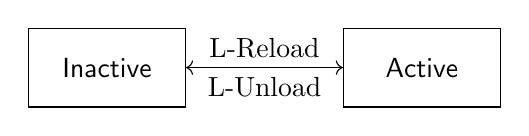
\begin{tikzpicture}[node distance=4cm, auto,
  state/.style={rectangle, draw, minimum width=2cm, minimum height=1cm}]
  \node[state] (inactive) {$\mathsf{Inactive}$};
  \node[state, right of=inactive] (active) {$\mathsf{Active}$};
  \draw[->] (inactive) -- node[above] {L-Reload} (active);
  \draw[->] (active) -- node[below] {L-Unload} (inactive);
\end{tikzpicture}
\caption{基础组件生命周期}\label{fig:4.1}
\end{figure}

\textbf{纤维。}一个组件可以被实例化多次，每次实例化携带自身的生命周期状态。我们将这样的实例化称为纤维。一个纤维记录产生它的组件、它在其下被实例化的纤维、它提供的协效应，以及它处于生命周期中的哪个位置。

\begin{definition}\label{def:4.2}
固定纤维名称的集合 $\mathfrak{N}$。实例化组件 $(d, p, e) \in \mathfrak{C}_\Gamma$ 的纤维是一个元组 $\langle d, p, e, \pi, \sigma, \tau, \theta\rangle$，其中
\begin{itemize}
\item $d: \mathfrak{D}_\Gamma$、$p: \mathfrak{P}_\Gamma$ 和 $e: \mathfrak{E}^*_\Gamma$ 是定义~\ref{def:4.1} 的协效应规范、供给和效应函数；
\item $\pi: \mathfrak{N} \cup \{\mathsf{root}\}$ 是父纤维，即此纤维在其下被实例化的纤维，或根标记 $\mathsf{root}$；
\item $\sigma: \Sigma$ 是纤维自身的协效应表（定义~22），在激活前为空，由其效应运行时写入；
\item $\tau: \{\bot, \top\}$ 是退役标志，$\bot$ 在新纤维中，$\top$ 在编排器退役该纤维后；
\item $\theta: \Theta_\Gamma$ 是生命周期状态，在第\S\ref{sec:4.2}节的两状态模型中为
\end{itemize}
\begin{equation}\label{eq:4.2}
\Theta_\Gamma \coloneqq \mathsf{Inactive} \mid \mathsf{Active}(g, \omega)
\end{equation}
其中 $g: \Gamma \to \Gamma$ 是累积器，$\omega: d \to \mathfrak{N}$ 是已提交视图。
\end{definition}

已提交视图 $\omega$ 将纤维声明的每个键发送到迁移提交时提供该键的纤维名称。第\S\ref{sec:4.3}节用进行中的迁移所需的扩展替换 $\Theta_\Gamma$；定义~\ref{def:4.2} 的其余部分对两者只给出一次，只是 $e$ 在第\S\ref{sec:4.3}节每一层引入的更丰富的效应类型上读取。

\textbf{注册表。}状态将其纤维保存在其名称下，纤维的身份和第3.2节的协效应上下文都是从该安排中读取的。

\begin{definition}\label{def:4.3}
用 $\mathfrak{F}_\Gamma$ 表示 $\Gamma$ 上的纤维集合。状态 $\gamma \in \Gamma$ 携带一个注册表
\begin{equation}\label{eq:4.3}
F_\gamma: \mathfrak{N} \rightharpoonup \mathfrak{F}_\Gamma
\end{equation}
一个有限部分函数，其父指针形成一棵以 $\mathsf{root}$ 为根的树，连同 $\Gamma$ 中没有被任何纤维的 $\sigma$ 命名的其余部分。我们将 $F_\gamma(n)$ 写作 $\gamma(n)$，并在状态明确时用 $n$ 作为下标缩写 $\gamma(n)$ 的字段，因此 $d_n$、$p_n$、$e_n$、$\pi_n$、$\sigma_n$、$\tau_n$、$\theta_n$ 是定义~\ref{def:4.2} 的字段，$g_n$、$\omega_n$ 是 $\theta_n$ 携带的累积器和已提交视图；$\gamma[\theta_n \mapsto \theta']$、$\gamma[n \mapsto \langle \cdots\rangle]$ 和 $\gamma \setminus n$ 分别是在一个字段、一个纤维和一个纤维的存在上与 $\gamma$ 不同的状态。
\end{definition}

纤维的名称赋予它一个经受自身变化的身份：下面的每条规则重写一个纤维的生命周期状态而保持其余不变，因此规则必须指明是哪一个，而有两个字段引用纤维而非描述它们，即父纤维 $\pi$ 和已提交视图 $\omega$。名称是原子：没有规则计算名称、检查其结构或通过除相等之外的任何关系关联两个名称，引入纤维只是抽取一个尚未使用的名称。这就是动态创建的局部名称的学科\cite{ref39}，在此用于纤维身份。

每个纤维拥有一张表意味着协效应上下文是推导出来的而非存储的：它是活跃纤维共同提供的。
\begin{equation}\label{eq:4.4}
\sigma_\gamma \coloneqq \bigcup \{\sigma_m \mid m \in \mathrm{dom}(F_\gamma),\, \theta_m = \mathsf{Active}(-, -)\}
\end{equation}
该并集是良定义的，因为纤维只写入其声明的键，$\mathrm{dom}(\sigma_n) \subseteq p_n$，且不同纤维的供给是不相交的（定义~\ref{def:4.1}），因此每个 $k \in \mathrm{dom}(\sigma_\gamma)$ 恰好位于一个 $\mathsf{Active}$ 纤维的表中，我们将其名称写作 $\mathrm{provider}_k(\gamma) \in \mathfrak{N}$，称为 $k$ 的提供者。因此每个键有一个可能的提供者，由供给而非状态固定。没有规则直接写入 $\sigma_n$：纤维的供给是其自身效应函数执行的集合操作，这些操作落入 $\sigma_n$ 并因此已是 $e_n$ 返回的状态的一部分，它们随累积器再次离开。只有效应的协效应部分以这种方式记录，因为只有协效应部分是其他纤维声明所针对的；在 $\gamma$ 其他地方改变状态的效应由 $g$ 像其他效应一样跟踪，但没有纤维可以在规范中命名它们，因此它们不贡献排序约束。

第3.2.2节的满足关系于是不变地适用，$\gamma \models d$ 缩写 $\sigma_\gamma \models d$。一个键恰好在某个 $\mathsf{Active}$ 纤维安装了它时位于 $\mathrm{dom}(\sigma_\gamma)$ 中，其供给是它可能安装的键而非已经安装的键，因此 $\gamma \models d$ 已要求每个声明的键都有一个 $\mathsf{Active}$ 提供者。仅对 $\mathsf{Active}$ 纤维取并集使得纤维可以在撤回任何内容之前停止提供，第\S\ref{sec:4.3.1}节将其转化为排序规则。

\subsection{基础演算}\label{sec:4.2}

本节给出图~\ref{fig:4.1} 的两状态生命周期的演算，别无其他：每个纤维被比较的目标，以及移动它的五条规则。

\textbf{目标视图。}规则将每个纤维与一个目标进行比较，即它是否应该正在运行以及针对其依赖的哪种解析。目标不仅是纤维本身的属性，因为纤维声明的键是对照整个状态解析的，所以它是该状态上的一个谓词。

\begin{definition}\label{def:4.4}
$n$ 在 $\gamma$ 处的目标视图将每个声明的键映射到其提供者，因此它是全映射 $d_n \to \mathfrak{N}$，当 $n$ 根本不应运行时为 $\bot$：
\begin{equation}\label{eq:4.5}
\mathrm{target}_n(\gamma) \coloneqq \begin{cases}
\bot & \text{if } \tau_n \lor \lnot(\gamma \models d_n) \\
(k \in d_n) \mapsto \mathrm{provider}_k(\gamma) & \text{otherwise}
\end{cases}
\end{equation}
\end{definition}

当每个纤维都已达到其目标视图时，状态是静止的：
\begin{equation}\label{eq:4.6}
\mathrm{quiet}(\gamma) \coloneqq \forall n \in \mathrm{dom}(F_\gamma).\, \begin{cases}
\mathrm{target}_n(\gamma) = \bot & \text{if } \theta_n = \mathsf{Inactive} \\
\mathrm{target}_n(\gamma) = \omega_n & \text{if } \theta_n = \mathsf{Active}(-, \omega_n)
\end{cases}
\end{equation}

目标只回应两件事：退役，通过 $\tau_n$；以及协效应解析，通过 $\gamma \models d_n$ 和 $\mathrm{provider}_k$，每个声明的键从定义~\ref{def:4.1} 的一个共享域中的 $\sigma_\gamma$ 读取。

定义~\ref{def:4.2} 的已提交视图与目标视图具有相同的类型，生命周期的驱动就是比较它们：$\omega_n$ 是 $n$ 激活时对照的解析，$\mathrm{target}_n(\gamma)$ 是它应该运行时对照的解析，下面的每条规则在它们相等或不同时触发。记录提供者而非值使得比较可用，因为否则提供相等值的不同纤维会比较相等。组件读取的值通过视图到达，因为提供者的表持有该值，实现在 \texttt{fiber.committed} 中持有该映射，在 \texttt{fiber.target} 中持有其哈希（第5.1.3节）。

\textbf{规则。}基础演算将每个迁移视为原子的、即时的和不会失败的：激活一步应用其效应函数，去激活一步应用累积器，两者都成功完成。第\S\ref{sec:4.3}节放弃这三个假设。

五条规则生成两个关系。编排规则，前缀 O-，写作 $\gamma \Rightarrow \delta$，是编排器可以执行的动作；其前提说明动作何时合法，而非何时发生。生命周期规则，前缀 L-，写作 $\gamma \longrightarrow \delta$，是系统在前提成立时无需提示即采取的步骤。步骤序列将两者交错，$\longrightarrow^*$ 在下文中仅指生命周期步骤。

\[
\frac{
\begin{array}{c}
n \notin \mathrm{dom}(F_\gamma) \\
\pi \in \mathrm{dom}(F_\gamma) \cup \{\mathsf{root}\} \\
(d, p, e) \in \mathfrak{C}_\Gamma \\
\forall m \in \mathrm{dom}(F_\gamma).\, p \cap p_m = \emptyset
\end{array}
}{
\gamma \Rightarrow \gamma[n \mapsto \langle d, p, e, \pi, \emptyset, \bot, \mathsf{Inactive}\rangle]
}\;\text{O-Insert}
\]

\[
\frac{n \in \mathrm{dom}(F_\gamma)}{
\gamma \Rightarrow \gamma[\tau_n \mapsto \top]
}\;\text{O-Retire}
\]

\[
\frac{
\begin{array}{c}
\tau_n = \top \\
\theta_n = \mathsf{Inactive} \\
\forall m.\, \pi_m \neq n
\end{array}
}{
\gamma \Rightarrow \gamma \setminus n
}\;\text{O-Remove}
\]

插入和退役是仅有的外部输入：编排器请求纤维存在或停止存在，从不直接设置其生命周期状态。O-Retire 对纤维的状态没有条件，因为退役是一个请求，生命周期规则负责执行它。退役与移除分离的原因相同：仍然 $\mathsf{Active}$ 的已退役纤维必须先被去激活，过早移除它会丢弃累积器并造成泄漏。前提 $\forall m.\, \pi_m \neq n$ 通过在父纤维之前移除子纤维来保持树的良构性。O-Insert 的最后一个前提是单源学科的施加之处：一个键有一个可能的提供者，因为编排器不允许第二个声明它的组件进入。

\[
\frac{
\begin{array}{c}
\theta_n = \mathsf{Inactive} \\
\omega = \mathrm{target}_n(\gamma) \neq \bot \\
e_n(\gamma) = (\delta, g)
\end{array}
}{
\gamma \longrightarrow \delta[\theta_n \mapsto \mathsf{Active}(g, \omega)]
}\;\text{L-Reload}
\]

\[
\frac{
\begin{array}{c}
\theta_n = \mathsf{Active}(g, \omega) \\
\mathrm{target}_n(\gamma) \neq \omega \\
g(\gamma) = \delta
\end{array}
}{
\gamma \longrightarrow \delta[\theta_n \mapsto \mathsf{Inactive}]
}\;\text{L-Unload}
\]

L-Reload 与逆一起安装已提交视图；L-Unload 应用逆并丢弃已提交视图。两者由相同的比较驱动：L-Reload 在纤维不持有已提交视图且其目标视图不为 $\bot$ 时触发，L-Unload 在其持有的已提交视图不是其目标视图时触发。这就是第3.2节的响应式规则，从一个同时回应退役和协效应的目标中读出：每当目标视图改变时就发起迁移，无论改变的来源是什么。

\textbf{实例化。}组件在安装其效应时可以实例化另一个组件，这就是插件宿主在插件加载自己的插件时所做的事情。到目前为止的规则将注册表留给编排规则独自处理，因此这样的实例化无处发生。一个原语为其提供场所。

\begin{definition}\label{def:4.5}
$e_n$ 的一次应用，或第\S\ref{sec:4.3.2}节适用时其一次迭代，可以注册一个组件 $(d, p, e) \in \mathfrak{C}_\Gamma$。代替状态映射，它以 $\pi = n$ 对该组件执行 O-Insert，并以其逆作为它产出的 O-Retire。规则抽取名称，受 O-Insert 的新鲜前提约束，并将其交给效应函数。
\end{definition}

逆是退役而非移除，原因是逆必须在到达的任何地方应用。O-Remove 带有前提，因此基于它构建的逆可能无法应用：子纤维仍然 $\mathsf{Active}$ 的父纤维无法运行其累积器，且没有规则会移动子纤维，因为定义~\ref{def:4.4} 不读取纤维树。O-Retire 以 $n \in \mathrm{dom}(F_\gamma)$ 作为其唯一前提。它在注册时的状态处留下的条目是退役的 $\mathsf{Inactive}(\bot)$，持有一个空表，这是引理~\ref{lem:4.4} 的残留条目：它仅在控制字段上与纤维的缺失不同，没有规则区分两者。

退役子纤维设置 $\tau$ 从而将其目标视图变为 $\bot$，此后普通规则将其带回 $\mathsf{Inactive}$。父纤维不需要等待，O-Retire 是无条件的，因此 L-Unload 无论子纤维是否已离开都适用于父纤维。孙纤维逐层到达，子纤维自身的累积器退役子纤维所注册的内容。定理~\ref{thm:4.5} 覆盖了这一级联以及第\S\ref{sec:4.3.1}节沿协效应施加的级联。

\textbf{约束。}有了这一个例外，效应函数所受的约束可以给出。它限定一次应用写入的内容，使得应用它的规则能说明其他所有变化；以及一次应用读取的内容，使得纤维看到它声明的协效应而不更多看到注册表。限定写入正是第\S\ref{sec:4.4}节能将表~\ref{tab:4.1} 读作写入的完整清单的原因。

\begin{definition}\label{def:4.6}
映射 $f: \Gamma \to \Gamma$ 被约束于 $n$，当对于每个 $n \in \mathrm{dom}(F_\gamma)$ 的 $\gamma \in \Gamma$，记 $\delta = f(\gamma)$，
\begin{enumerate}
\item （写入。）$\mathrm{dom}(F_\delta) = \mathrm{dom}(F_\gamma)$，对每个 $m \in \mathrm{dom}(F_\gamma)$ 且 $m \neq n$ 有 $\delta(m) = \gamma(m)$，且 $\delta(n)$ 和 $\gamma(n)$ 仅在 $\sigma$ 上不同；
\item （读取。）两个在 $\sigma_n$、对每个 $m \in \mathrm{dom}(F_\gamma)$ 的限制 $\sigma_m|_{d_n}$、以及没有被任何纤维的表命名的状态部分上相同的状态，被 $f$ 映射到在相同三者上相同的两个状态。
\end{enumerate}
效应函数 $e$ 被约束于 $n$，当其每次应用以及第\S\ref{sec:4.3.2}节适用时的每次迭代，要么注册一个组件（定义~\ref{def:4.5}），要么其状态映射 $\mathrm{pr}_1 \circ e$ 和它产出的逆都被约束于 $n$。每个纤维的效应函数都要求被约束于该纤维。
\end{definition}

注册写入 O-Insert 写入的条目，在其抽取的名称处，不写入其他内容；它作为逆产出的 O-Retire 写入该名称的 $\tau$，不写入其他内容。因此两种应用都不写入已存在纤维的控制字段，除了那一个 $\tau$，也不读取任何控制字段。

条款 (2) 是组件可以读取其声明的值的原因：这些值位于其提供者的表中，因此不读取 $\sigma_n$ 以外的表的效应函数将无法使用其自身的协效应。它不能读取的是 $d_n$ 之外的表，或任何控制字段，这正是阻止组件根据其未声明的纤维的生命周期状态进行分支的原因。

规则是非确定性的：多个纤维可能持有与其目标视图不同的已提交视图，关系不承诺它们之间的顺序。规则也仅是响应式的，没有规则提及调度器；步骤是规则应用的任何序列，因此在所有此类序列上证明的定理对运行时可能采用的任何调度策略都成立。

\subsection{进行中的迁移}\label{sec:4.3}

本节在四个方面扩展基础演算。第一个提供第3.2节要求而第\S\ref{sec:4.2}节无法表达的内容，即一个扩展在其依赖者可能占据的时间间隔上的去激活；其他三个放弃迁移是原子的、即时的和不会失败的理想化假设，而真实运行时中的迁移三者皆非。被放弃的是整个迁移是一个步骤，而不是一个步骤是一次规则应用，四者共享一个结构性后果，在此一次给出：不是一步的迁移需要一个在进行时占据的状态，为其可能运行的每个方向各一个。

\begin{definition}\label{def:4.7}
本节的生命周期状态将 $\Theta_\Gamma$ 替换为
\begin{equation}\label{eq:4.7}
\Theta_\Gamma \coloneqq \mathsf{Inactive}(\zeta) \mid \mathsf{Reloading}(i, g, \omega) \mid \mathsf{Active}(g, \omega) \mid \mathsf{Unloading}(g, \omega, \zeta)
\end{equation}
其中 $i: \mathfrak{E}^{\mathrm{iter}^*}_\Gamma$ 是剩余效应迭代器（下文定义~\ref{def:4.9}），$g: \Gamma \to \Gamma$ 是目前已构建的累积器，$\omega: d \to \mathfrak{N}$ 是已提交视图，$\zeta: \{\bot\} \cup \Xi$ 是结果，由 $\mathsf{Unloading}$ 携带为其去激活所趋向的结果，由 $\mathsf{Inactive}$ 携带为其已达到的结果，要么是 $\bot$，要么是从第\S\ref{sec:4.3.4}节提供的错误集合 $\Xi$ 中抽取的错误。
\end{definition}

纤维在处于携带累积器和已提交视图的三个状态之一时是已安装的，在携带错误结果时是失败的：
\begin{equation}\label{eq:4.8}
\mathrm{installed}_n(\gamma) \coloneqq \theta_n \neq \mathsf{Inactive}(-),\quad \mathrm{failed}_n(\gamma) \coloneqq \exists \xi \in \Xi.\, \theta_n = \mathsf{Inactive}(\xi)
\end{equation}
已安装的纤维 $n$ 在 $\omega_n(k) = m$ 时将 $k$ 解析到 $m$。定义~\ref{def:4.4} 的静止性在更宽的状态空间上读作
\begin{equation}\label{eq:4.9}
\mathrm{quiet}(\gamma) \coloneqq \forall n \in \mathrm{dom}(F_\gamma).\, \begin{cases}
\zeta \neq \bot \lor \mathrm{target}_n(\gamma) = \bot & \text{if } \theta_n = \mathsf{Inactive}(\zeta) \\
\mathrm{target}_n(\gamma) = \omega_n & \text{if } \theta_n = \mathsf{Active}(-, \omega_n) \\
\bot & \text{otherwise}
\end{cases}
\end{equation}

第\S\ref{sec:4.1}节的定义延续到该状态空间，有两处读取需要确定。第一，第\S\ref{sec:4.2}节的 $\mathsf{Inactive}$ 在 O-Insert 的结论中读作 $\mathsf{Inactive}(\bot)$，在 O-Remove 的前提中读作 $\mathsf{Inactive}(-)$。第二，$\sigma_\gamma$ 仍然仅对 $\mathsf{Active}$ 纤维的表取并集，因此一个其迁移在任一方向进行中的纤维通过其持有的 $\omega$ 读取协效应而不提供自己的协效应；其迁移已经写入的键因此还不是依赖者可以激活所对照的键。在两状态演算中这一区分是空的，每个已安装的纤维在那里都是 $\mathsf{Active}$ 的。

图~\ref{fig:4.2} 绘制了这些状态形成的生命周期，以下四个子节提供其边上的规则。

\begin{figure}[htbp]
\centering
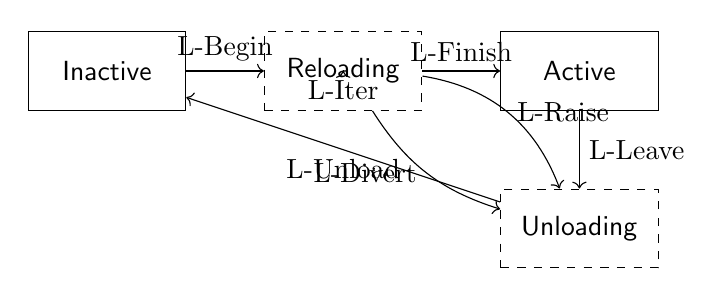
\begin{tikzpicture}[node distance=3cm, auto,
  state/.style={rectangle, draw, minimum width=2cm, minimum height=1cm},
  transstate/.style={rectangle, draw, dashed, minimum width=2cm, minimum height=1cm}]
  \node[state] (inactive) {$\mathsf{Inactive}$};
  \node[transstate, right of=inactive, node distance=3cm] (reloading) {$\mathsf{Reloading}$};
  \node[state, right of=reloading, node distance=3cm] (active) {$\mathsf{Active}$};
  \node[transstate, below of=active, node distance=2cm] (unloading) {$\mathsf{Unloading}$};
  \draw[->] (inactive) -- node[above] {L-Begin} (reloading);
  \draw[->] (reloading) -- node[above] {L-Finish} (active);
  \draw[->] (active) -- node[right] {L-Leave} (unloading);
  \draw[->] (unloading) -- node[below] {L-Unload} (inactive);
  \draw[->, bend left=20] (reloading) to node[below] {L-Iter} (reloading);
  \draw[->, bend right=20] (reloading) to node[left] {L-Divert} (unloading);
  \draw[->, bend left=30] (reloading) to node[right] {L-Raise} (unloading);
\end{tikzpicture}
\caption{带进行中迁移的生命周期；两个迁移状态以虚线框标出}\label{fig:4.2}
\end{figure}

\subsubsection{撤回}\label{sec:4.3.1}

第3.2节要求依赖者在其依赖之后激活，依赖仅在其依赖者去激活之后撤回其供给。前半部分在基础演算中已经成立：激活要求 $\gamma \models d_n$，因此声明 $k$ 的纤维不能在某个纤维活跃提供 $k$ 之前激活。后半部分是实质性的，它必须交付的不仅是状态变化的排序。一个因其提供者即将离开而被拆卸的组件正在运行其自身的拆卸代码，这可能恰好需要正在被撤回的协效应；关闭连接池通常意味着将连接交还给提供它们的一方。后半部分必须交付的是消费者在整个去激活过程中仍然可以读取 $k$，且提供者对 $k$ 的撤回仅在此之后生效。基础演算完全无法交付这一点：其 L-Unload 将供给的移除和逆的运行放在一起，两者之间没有间隔供消费者的拆卸占据。

本层将该步骤一分为二，并用以下条件守护后半部分。

\begin{definition}\label{def:4.8}
纤维 $n$ 在 $\gamma$ 处被依赖，当某个其他已安装的纤维将一个键解析到它：
\begin{equation}\label{eq:4.10}
\mathrm{relied}_n(\gamma) \coloneqq \exists m \in \mathrm{dom}(F_\gamma), k \in d_m.\, m \neq n \land \mathrm{installed}_m(\gamma) \land \omega_m(k) = n
\end{equation}
\end{definition}

\[
\frac{
\begin{array}{c}
\theta_n = \mathsf{Active}(g, \omega) \\
\mathrm{target}_n(\gamma) \neq \omega
\end{array}
}{
\gamma \longrightarrow \gamma[\theta_n \mapsto \mathsf{Unloading}(g, \omega, \bot)]
}\;\text{L-Leave}
\]

\[
\frac{
\begin{array}{c}
\theta_n = \mathsf{Unloading}(g, \omega, \zeta) \\
\lnot\, \mathrm{relied}_n(\gamma) \\
g(\gamma) = \delta
\end{array}
}{
\gamma \longrightarrow \delta[\theta_n \mapsto \mathsf{Inactive}(\zeta)]
}\;\text{L-Unload}
\]

L-Leave 记录去激活的决定而不执行，这使纤维停止提供其协效应，同时保持其自身的已提交视图和其他所有人的已提交视图完好。L-Unload 应用累积器，丢弃已提交视图，使纤维以其携带的结果变为 $\mathsf{Inactive}$；结果为 $\bot$ 直到第\S\ref{sec:4.3.4}节提供其他情况。它是演算中唯一应用累积器的规则。

排序的两半由此由形式的不同部分承载：可见性半由已提交视图承载，L-Unload 以其最后操作丢弃它；排序半由前提 $\lnot\, \mathrm{relied}_n(\gamma)$ 承载，我们称之为守卫，它将 $k$ 的撤回推迟到每个将其解析到 $n$ 的消费者都已离开之后。定理~\ref{thm:4.3} 建立了这两点。

守卫是按绑定施加而非按纤维施加的：$\mathrm{relied}_n(\gamma)$ 测试是否有某个已提交视图命名 $n$，因此不声明 $n$ 的任何键的纤维不是障碍，在另一个域中解析了 $n$ 的某个键的纤维也不是障碍（第3.2.3节）。在第\S\ref{sec:4.2}节的单源学科下，按绑定的读取与更粗的测试 $\exists m \neq n, k \in d_m.\, \mathrm{installed}_m(\gamma) \land k \in p_n$ 一致，一个键在那里只有一个可能的提供者。

这种守卫通常会死锁。使其不死锁的是 $\mathsf{Unloading}$ 连同 $\sigma_\gamma$ 仅对 $\mathsf{Active}$ 纤维取并集：一旦 L-Leave 标记了 $n$，其表离开 $\sigma_\gamma$，因此没有目标视图能再命名 $n$，每个承诺于 $n$ 的消费者自身也在退出的路上。定理~\ref{thm:4.5} 将此转化为守卫总是释放的断言。

守卫沿协效应排序去激活而非沿纤维树：父纤维可以在其子纤维仍然 $\mathsf{Unloading}$ 时运行其逆，因为 $\mathrm{relied}$ 仅涉及已提交视图。父纤维和子纤维因此比定理~\ref{thm:4.3} 排序提供者及其消费者的方式更弱，父纤维和子纤维在环境状态中的效应交集由定义~\ref{def:4.10} 的独立性假设管理。

\subsubsection{迭代}\label{sec:4.3.2}

一次激活可以顺序执行多个效应，去激活必须恢复它们。我们用效应迭代器对此类激活建模，其每次迭代产出修改后的上下文、一个逆和一个续延：

\begin{definition}\label{def:4.9}
定义效应迭代器 $\mathfrak{E}^{\mathrm{iter}}_\Gamma$ 和见证效应迭代器 $\mathfrak{E}^{\mathrm{iter}^*}_\Gamma$ 为以下递归类型：
\begin{equation}\label{eq:4.11}
\mathfrak{E}^{\mathrm{iter}}_\Gamma \coloneqq \mu \mathfrak{I}.\, \Gamma \to \Gamma \times (\Gamma \to \Gamma) \times \mathsf{Maybe}(\mathfrak{I})
\end{equation}
\begin{equation}\label{eq:4.12}
\mathfrak{E}^{\mathrm{iter}^*}_\Gamma \coloneqq \mu \mathfrak{I}.\, (e: \Gamma \to \Gamma \times (\Gamma \to \Gamma) \times \mathsf{Maybe}(\mathfrak{I})) \times ((\gamma: \Gamma) \to (\mathbf{let}\,(\delta, g, o) = e(\gamma)\,\mathbf{in}\, g(\delta) \simeq \gamma))
\end{equation}
其中 $e(\gamma)$ 产出三元组 $(\delta, g, o)$，表示：
\begin{itemize}
\item $\delta$ 是新上下文；
\item $g$ 是当前效应的逆函数；
\item $o$ 指示续延：
\begin{itemize}
\item $\mathsf{Nothing}$ 表示迭代终止；
\item $\mathsf{Just}(i)$ 提供下一次迭代。
\end{itemize}
\end{itemize}
见证在定义~33 的 $\simeq$ 处读取，正如定义~37 读取 $\mathfrak{E}^*_\Gamma$ 的见证：$i \in \mathfrak{E}^{\mathrm{iter}}_\Gamma$ 在 $i$ 尊重 $\simeq$ 且其产出的每个 $g$ 尊重 $\simeq$ 并满足上述条款时属于 $\mathfrak{E}^{\mathrm{iter}^*}_\Gamma$。三元组逐分量比较，$\mathsf{Nothing}$ 仅与 $\mathsf{Nothing}$ 比较，$\mathsf{Just}(i)$ 在 $i \simeq i'$ 时与 $\mathsf{Just}(i')$ 比较，$\simeq$ 在迭代器上是满足这些条款的最大关系。将 $\simeq$ 取为 $\Gamma$ 上的相等性即可精确恢复读取。
\end{definition}

效应迭代器变换 $\mathrm{effect}^{\mathrm{iter}}_\Gamma$ 通过递归调用将 $\mathrm{effect}_\Gamma$ 扩展到迭代器结构：

\begin{definition}\label{def:4.10}
定义效应迭代器变换 $\mathrm{effect}^{\mathrm{iter}}_\Gamma$ 为：
\begin{equation}\label{eq:4.13}
\mathrm{effect}^{\mathrm{iter}}_\Gamma: \mathfrak{E}^{\mathrm{iter}}_\Gamma \to \partial\Gamma \to \partial^2\Gamma
\end{equation}
\[
\mathrm{effect}^{\mathrm{iter}}_\Gamma = i \mapsto (\gamma, \varphi) \mapsto \mathbf{let}\,(\delta, g, o) = i(\gamma)\,\mathbf{in}\, \mathbf{let}\,t = \mathrm{track}_\Gamma(g, \mathrm{pr}_1 \circ i)\,\mathbf{in}\, \mathbf{match}\,o
\]
\[
\mid \mathsf{Nothing} \Rightarrow ((\delta, \varphi \circ g), t)
\]
\[
\mid \mathsf{Just}(i') \Rightarrow \mathbf{let}\,(s, r) = \mathrm{effect}^{\mathrm{iter}}_\Gamma(i')(\delta, \varphi \circ g)\,\mathbf{in}\, (s, t \circ r)
\]
\end{definition}

在每次迭代中，逆 $g$ 按应用顺序组合到 $\varphi$ 上，因此累积器 $\varphi \circ g_1 \circ \cdots \circ g_k$ 在应用时自然以后进先出的顺序恢复效应。因为 $\mathrm{effect}^{\mathrm{iter}}_\Gamma$ 落在与 $\mathrm{effect}_\Gamma$ 相同的 $\partial\Gamma \to \partial^2\Gamma$ 中，迭代器本身就是一种效应，可以在效应可用的任何地方使用。组件的整个激活就是这样一种使用，这就是本节其余部分形式化的内容，实现在每个变异点都接受迭代器（第5.1.1节）。$\mathsf{Maybe}(\mathfrak{E}^{\mathrm{iter}})$ 续延在任意两次连续迭代之间提供了一个边界，在边界处上下文是到目前为止的迭代所产生的，累积器恢复这些而不更多。在这个意义上，效应迭代器是一个具体化的定界续延，主流语言通过 \texttt{yield} 运算符暴露的结构\cite{ref43}，因此模型直接映射到它们已提供的生成器。

在演算中，定义~\ref{def:4.2} 的 $e_n$ 从此处在 $\mathfrak{E}^{\mathrm{iter}^*}_\Gamma$ 上读取，用迭代器替代原子效应函数将基础 L-Reload 分裂为轨迹经过的一个开始状态，并给纤维从该状态退出的第二种方式。

\[
\frac{
\begin{array}{c}
\theta_n = \mathsf{Inactive}(\bot) \\
\omega = \mathrm{target}_n(\gamma) \neq \bot
\end{array}
}{
\gamma \longrightarrow \gamma[\theta_n \mapsto \mathsf{Reloading}(e_n, \mathrm{id}_\Gamma, \omega)]
}\;\text{L-Begin}
\]

\[
\frac{
\begin{array}{c}
\theta_n = \mathsf{Reloading}(i, g, \omega) \\
\mathrm{target}_n(\gamma) \neq \omega \\
(\delta, h) = (\gamma, \mathrm{id}_\Gamma) \lor i(\gamma) = (\delta, h, -)
\end{array}
}{
\gamma \longrightarrow \delta[\theta_n \mapsto \mathsf{Unloading}(g \circ h, \omega, \bot)]
}\;\text{L-Divert}
\]

\[
\frac{
\begin{array}{c}
\theta_n = \mathsf{Reloading}(i, g, \omega) \\
\mathrm{target}_n(\gamma) = \omega \\
i(\gamma) = (\delta, h, \mathsf{Just}(i'))
\end{array}
}{
\gamma \longrightarrow \delta[\theta_n \mapsto \mathsf{Reloading}(i', g \circ h, \omega)]
}\;\text{L-Iter}
\]

\[
\frac{
\begin{array}{c}
\theta_n = \mathsf{Reloading}(i, g, \omega) \\
\mathrm{target}_n(\gamma) = \omega \\
i(\gamma) = (\delta, h, \mathsf{Nothing})
\end{array}
}{
\gamma \longrightarrow \delta[\theta_n \mapsto \mathsf{Active}(g \circ h, \omega)]
}\;\text{L-Finish}
\]

每次迭代将新产出的逆组合到累积器上为 $g \circ h$，遵循定义~\ref{def:4.10}，因此累积器以后进先出的顺序应用逆。在任意两次连续迭代之间，系统可以在目标视图改变时转移迁移，将目前已累积的逆应用于恢复上下文。L-Divert 像每个其他去激活一样路由通过 $\mathsf{Unloading}$，而不是在原位应用累积器，它在那里遇到的守卫是空的，一个从未 $\mathsf{Active}$ 的纤维不提供任何内容也不出现在任何已提交视图中。它的两个选择中的第一个中止纤维持有的迭代，这只有迭代边界才使之可能，因此转移可能落下的粒度就是迭代器的粒度；第二个让该迭代着陆，第\S\ref{sec:4.3.3}节正是需要它的地方。

普通的效应函数（$\mathfrak{E}_\Gamma$）是退化情况，其第一次迭代已产出 $\mathsf{Nothing}$。这样的迁移仍然经过 $\mathsf{Reloading}$，L-Divert 仍然在那里适用，但累积器是 $\mathrm{id}_\Gamma$ 且没有迭代运行过，因此没有恢复任何内容，迁移要么安装其全部效应，要么一个都不安装。

\subsubsection{异步性}\label{sec:4.3.3}

到目前为止的层允许环境在迭代之间移动，并假设每次迭代本身即时完成，其启动和着陆是一个步骤。我们抽象地建模非即时性：一次迭代产出类型为 $\mathsf{Future}(A)$ 的值，其中 $\mathsf{Future}$ 是一个不透明类型构造子，其定义性质是在提交和解析之间外部状态可能改变。

在此模型下，一次迭代在一个状态启动并在另一个状态着陆，而纤维在飞行中处于 $\mathsf{Reloading}$。本层增加的是惯性：一旦启动，迭代就着陆，其着陆不能被拒绝。因此在飞行期间转向的目标视图不能通过中止迭代来回应，只有着陆一个迭代的 L-Divert 的替代选择仍然可用：迭代着陆，纤维随后去激活。因此本层不增加规则，也不增加规则匹配的类型；在 $\Gamma$ 的粒度上惯性就是其全部内容，它采取对 L-Divert 的哪个替代选择宿主可以采取的限制形式。

那个替代选择正是基础演算无法表达的。在那里，目标视图已转向的迁移在发现转向的同一步中被撤销；这里飞行中的迭代必须先着陆，因此纤维需要在运行其逆时有一个地方待，唯一合理的位置是 $\mathsf{Unloading}$ 持有迭代产出的逆。改为路由通过 $\mathsf{Active}$ 会让纤维在一个步骤的长度内提供其协效应，并迫使依赖者激活对照一个已经在离开的组件。这就是实现中重载和卸载的互链。

去激活也可以通过复合而非规则直接链回激活。L-Unload 对目标视图没有前提，因此无论纤维去激活期间目标视图变成什么，累积器运行且纤维变为 $\mathsf{Inactive}$，L-Begin 可以立即从那里开始新的迁移。

\subsubsection{失败}\label{sec:4.3.4}

到目前为止的每条规则都假设其运行的效应成功，而运行时做不到这一点。组件安装的效应到达跟踪它们的上下文之外，到达的部分可能拒绝：一个已绑定的端口、一个不存在的文件、一个不响应的对端。失败的迁移仍然必须使纤维的效应被恢复而非搁浅。

设 $\Xi$ 为错误集合，将定义~\ref{def:4.9} 的效应迭代器细化使得迭代可以抛出异常而非产出三元组：
\begin{equation}\label{eq:4.15}
\mathfrak{E}^{\mathrm{fail}}_\Gamma \coloneqq \mu \mathfrak{I}.\, \Gamma \to \mathsf{Either}(\Xi, \Gamma \times (\Gamma \to \Gamma) \times \mathsf{Maybe}(\mathfrak{I}))
\end{equation}
\begin{equation}\label{eq:4.16}
\mathfrak{E}^{\mathrm{fail}^*}_\Gamma \coloneqq \mu \mathfrak{I}.\, (e: \Gamma \to \mathsf{Either}(\Xi, \Gamma \times (\Gamma \to \Gamma) \times \mathsf{Maybe}(\mathfrak{I}))) \times ((\gamma: \Gamma) \to (\mathbf{let}\,\mathsf{Right}(\delta, g, o) = e(\gamma)\,\mathbf{in}\, g(\delta) \simeq \gamma))
\end{equation}
见证仅约束 $\mathsf{Right}$ 的情况，在模式不匹配处是空的，抛出异常没有需要撤销的内容，$\mathsf{Reloading}$ 携带的 $i$ 从此处在 $\mathfrak{E}^{\mathrm{fail}^*}_\Gamma$ 上读取。定义~\ref{def:4.10} 的提升以抛出异常替代三元组传播的方式延续，因此抛出异常的迭代器可以在效应可用的任何地方使用，正如普通迭代器一样。本层增加一条规则并将定义~\ref{def:4.7} 的第二个结果投入使用，O-Remove 不需要加宽即可接受它。L-Iter、L-Finish 和 L-Divert 的前提在它们匹配的三元组周围读取 $\mathsf{Right}$。抛出异常是迭代所做的事情，因此规则是从 $\mathsf{Reloading}$ 的出口。

\[
\frac{
\begin{array}{c}
\theta_n = \mathsf{Reloading}(i, g, \omega) \\
i(\gamma) = \mathsf{Left}(\xi)
\end{array}
}{
\gamma \longrightarrow \gamma[\theta_n \mapsto \mathsf{Unloading}(g, \omega, \xi)]
}\;\text{L-Raise}
\]

L-Raise 在记录之前先恢复。纤维路由进入 $\mathsf{Unloading}$ 携带错误作为其结果，到失败迭代为止构建的累积器在那里应用，纤维到达 $\mathsf{Inactive}(\xi)$ 时没有安装任何内容，在与中止的 L-Divert 所产生的状态仅在纤维携带的结果上不同的状态处。像每个其他去激活一样路由失败是使得每个结果仅通过 L-Unload 可达的单一事实，定理~\ref{thm:4.1} 正以此为基础。L-Begin 以 $\mathsf{Inactive}(\bot)$ 为前提，因此生命周期不从错误结果重新进入；这是结果的实质，它阻止了一个效应函数已表明在运行时所对照的状态中不可靠的纤维被重试对照不变的环境。失败的纤维也不阻碍任何东西：它是 $\mathsf{Inactive}$ 的，因此不携带已提交视图，也不能使 $\mathrm{relied}$ 成立。

失败记录在纤维上而非传播到其父纤维，因此迁移失败的组件让其兄弟继续运行，这是插件宿主想要的行为，也是结果按纤维设置而非整个状态属性的原因。

\subsection{元理论}\label{sec:4.4}

第\S\ref{sec:4.3}节提供十条规则：第\S\ref{sec:4.2}节的三条编排规则；L-Begin、L-Iter 和 L-Finish 用于激活；L-Divert 和 L-Raise 用于激活可能提前结束的两种方式；以及 L-Leave 和 L-Unload 用于去激活。本节从这些规则中以全局形式读出可组合性的两个维度，一个纤维的保证在其他纤维之间的任何操作下都成立，并添加只有整个系统才能被要求的内容：它总是到达其目标所要求的配置，且该配置是静态组装本会产生的配置。下面的每个性质都是步骤序列的性质，因此我们索引步骤并从该索引读取状态的字段。

两个约定将第3.3.2节延续到本节。下面状态之间的每个相等都在定义~33 的观察等价 $\simeq$ 下读取，正如引理~38 读取第3.1节的那些，效应函数所受的见证条件是定义~37 给出的那个，对迭代器按定义~\ref{def:4.9} 读取，对注册迭代在下文的 $\approx$ 处读取。

\begin{definition}\label{def:4.11}
用 $t$ 索引步骤，使得 $\gamma_t$ 是前 $t$ 步到达的状态，并记
\begin{equation}\label{eq:4.17}
\mathrm{step}_t \coloneqq r(n)
\end{equation}
为在 $\gamma_t$ 处采取的步骤：它应用的规则 $r$，十条之一，以及它应用该规则的名称 $n \in \mathfrak{N}$。序列从一个 $\gamma_0$ 开始，$\mathrm{dom}(F_0) = \emptyset$，因此每个纤维通过 O-Insert 进入存在，无论是编排器的还是迭代所采取的（定义~\ref{def:4.5}）。$\gamma_t$ 的字段携带索引作为上标，因此 $\theta^t_n$、$\omega^t_n$、$\sigma^t_n$、$g^t_n$ 和 $i^t_n$ 是 $n$ 在 $\gamma_t$ 处的生命周期状态、已提交视图、表、累积器和剩余迭代器，$F^t$ 和 $\sigma^t$ 是 $\gamma_t$ 本身的注册表和协效应上下文，即定义~\ref{def:4.3} 在那里读取的 $F_\gamma$ 和 $\sigma_\gamma$。谓词以状态为参数、其余为下标，因此 $\mathrm{installed}^t_n$、$\mathrm{target}^t_n$、$\mathrm{relied}^t_n$ 和 $\mathrm{quiet}^t$ 是定义~\ref{def:4.4}、定义~\ref{def:4.7} 和定义~\ref{def:4.8} 在 $\gamma_t$ 处的谓词。$n$ 的一个片段是索引的最大区间 $[b, u]$，在其中 $\mathrm{installed}^t_n$ 成立。它在 $b$ 处开启，其中 $b > 0$ 且 $\lnot\,\mathrm{installed}^{b-1}_n$，空的 $F_0$ 使得开始时没有纤维被安装；它在 $u$ 处关闭当 $\mathrm{installed}^u_n$ 且 $\lnot\,\mathrm{installed}^{u+1}_n$，最终片段不需要这样做。
\end{definition}

第\S\ref{sec:4.3}节的每条规则结论的形状为 $\gamma \longrightarrow \delta[\cdots]$，其中前提从 $\gamma$ 计算 $\delta$ 并在未计算时将其留作 $\gamma$，方括号编辑注册表的命名字段。两半分别命名，两者都是整个 $\Gamma$ 上的映射。在 $\gamma_t$ 处由作用于 $n$ 的规则所采取的步骤的状态映射为
\begin{equation}\label{eq:4.18}
\Psi_t \coloneqq \begin{cases}
\mathrm{pr}_1 \circ i & \mbox{在 L-Iter、L-Finish 和着陆的 L-Divert 处} \\
g & \mbox{在 L-Unload 处} \\
\mathrm{id}_\Gamma & \mbox{在所有其他规则处}
\end{cases}
\end{equation}
其中 $i$ 和 $g$ 是 $\theta^t_n$ 携带的迭代器和累积器，编辑 $\mathrm{edit}_t: \Gamma \to \Gamma$ 是方括号作为函数读取，赋予它命名的字段以在 $\gamma_t$ 处前提计算的值。两者因此由 $\mathrm{step}_t$ 连同 $\gamma_t$ 固定并在每个状态上定义，这正是定理~\ref{thm:4.7} 和引理~\ref{lem:4.9} 能在远离 $\gamma_t$ 处求值它们的原因。每一步分解为
\begin{equation}\label{eq:4.19}
\gamma_{t+1} = \mathrm{edit}_t(\Psi_t(\gamma_t))
\end{equation}
例如在 L-Unload 处，$\mathrm{edit}_t$ 是 $[\theta_n \mapsto \mathsf{Inactive}(\zeta)]$，在 O-Remove 处是移除 $\setminus n$，这就是为什么后半是编辑而非赋值。字段沿着相同的接缝划分：表 $\sigma_m$，一旦创建 $m$ 的 O-Insert 将其设为空后不再有 $\mathrm{edit}_t$ 写入；控制字段 $\theta_m$、$\tau_m$、$\pi_m$、$d_m$、$p_m$、$e_m$ 连同 $\mathrm{dom}(F_\gamma)$，除了通过定义~\ref{def:4.5} 的原语外不再有 $\Psi_t$ 写入。记 $\gamma \approx \delta$ 当两个状态在除控制字段外的一切上相同。

关系 $\approx$ 不是定义~33 的 $\simeq$，两者互不精化，因为各自忘记了对方必须保留的内容。恢复精确性是关于效应的声明，因此 $\approx$ 精确比较表和环境状态，仅忘记注册表记录哪个纤维安装了它们。规则读取控制字段来决定是否适用，因此 $\simeq$ 必须保留它们，本节将其读取为定义~33 与注册表域上的一致以及每个纤维的每个控制字段上的一致的合取：
\begin{equation}\label{eq:4.20}
\gamma \simeq \delta \coloneqq \sigma_\gamma \simeq \sigma_\delta \land \mathrm{dom}(F_\gamma) = \mathrm{dom}(F_\delta) \land \forall n, c \in \{\theta, \tau, \pi, d, p, e\}.\, c(\gamma(n)) \simeq c(\delta(n))
\end{equation}
函数类型的字段，如 $e_n$ 和 $\theta_n$ 内部的 $g$，按定义~36 比较映射的方式比较，迭代器按定义~\ref{def:4.9} 比较两个迭代器的方式比较，其他类型的字段按相等性比较。下面的结果在两个关系下都成立，一个用于状态的每一半，引理~\ref{lem:4.3} 对所有十条规则一次性建立 $\simeq$ 的那一半。

表~\ref{tab:4.1} 是第\S\ref{sec:4.3}节的十条规则作为此类写入的读取。累积器、已提交视图和剩余迭代器是 $\theta_n$ 的组成部分，因此第三列也记录对它们的写入，$h$ 在那里命名第四列的迭代产出的逆，$\mathrm{id}_\Gamma$ 在 L-Divert 中止该迭代处。在从迭代器构建的 $\Psi_t$ 注册纤维（定义~\ref{def:4.5}）处，该注册在其抽取的名称处携带 O-Insert 行的写入，累积器退役一个纤维的 L-Unload 携带 O-Retire 行的写入。下面的每个分情况分析都是表中的查找，五个查找频繁出现足以命名。

\begin{table}[htbp]
\centering
\caption{规则作为对其所作用的纤维 $n$ 的写入，其中 $\mathrm{step}_t$ 是在 $n$ 处应用该规则}\label{tab:4.1}
\begin{tabular}{lllll}
\hline
规则 & $\theta^t_n$ & $\theta^{t+1}_n$ & $\Psi_t$ & 编辑的控制字段 \\
\hline
O-Insert & undefined & $\mathsf{Inactive}(\bot)$ & $\mathrm{id}_\Gamma$ & $\mathrm{dom}(F_\gamma)$ \\
O-Retire & unconstrained & unchanged & $\mathrm{id}_\Gamma$ & $\tau_n$ \\
O-Remove & $\mathsf{Inactive}(-)$ & undefined & $\mathrm{id}_\Gamma$ & $\mathrm{dom}(F_\gamma)$ \\
L-Begin & $\mathsf{Inactive}(\bot)$ & $\mathsf{Reloading}(e_n, \mathrm{id}_\Gamma, \omega)$ & $\mathrm{id}_\Gamma$ & $\theta_n$ \\
L-Iter & $\mathsf{Reloading}(i, g, \omega)$ & $\mathsf{Reloading}(i', g \circ h, \omega)$ & $\mathrm{pr}_1 \circ i$ & $\theta_n$ \\
L-Finish & $\mathsf{Reloading}(i, g, \omega)$ & $\mathsf{Active}(g \circ h, \omega)$ & $\mathrm{pr}_1 \circ i$ & $\theta_n$ \\
L-Divert & $\mathsf{Reloading}(i, g, \omega)$ & $\mathsf{Unloading}(g \circ h, \omega, \bot)$ & $\mathrm{id}_\Gamma$ 或 $\mathrm{pr}_1 \circ i$ & $\theta_n$ \\
L-Raise & $\mathsf{Reloading}(i, g, \omega)$ & $\mathsf{Unloading}(g, \omega, \xi)$ & $\mathrm{id}_\Gamma$ & $\theta_n$ \\
L-Leave & $\mathsf{Active}(g, \omega)$ & $\mathsf{Unloading}(g, \omega, \bot)$ & $\mathrm{id}_\Gamma$ & $\theta_n$ \\
L-Unload & $\mathsf{Unloading}(g, \omega, \zeta)$ & $\mathsf{Inactive}(\zeta)$ & $g$ & $\theta_n$ \\
\hline
\end{tabular}
\end{table}

\begin{lemma}\label{lem:4.1}
连同定义~\ref{def:4.6} 读取表~\ref{tab:4.1}，对于每一步 $t$ 和 $\gamma_t$ 处的所有纤维 $m$、$n$：
\begin{enumerate}
\item $\sigma^{t+1}_m \neq \sigma^t_m$ 仅在步骤 $t$ 作用于 $m$ 处，写入位于 $\Psi_t$ 内部；
\item $\omega_n$ 仅在 $\mathrm{step}_t = \text{L-Begin}(n)$ 处进入存在，仅在 $\mathrm{step}_t = \text{L-Unload}(n)$ 处消失，因此 $\omega^t_n$ 在 $n$ 的一个片段中对 $t$ 是常量；
\item $\Psi_t = g^t_n$ 仅在 $\mathrm{step}_t = \text{L-Unload}(n)$ 处，没有其他步骤将 $g_n$ 应用于状态；
\item $\lnot\,\mathrm{installed}^t_n \land \mathrm{installed}^{t+1}_n \Rightarrow \mathrm{step}_t = \text{L-Begin}(n)$，且 $\mathrm{installed}^t_n \land \lnot\,\mathrm{installed}^{t+1}_n \Rightarrow \mathrm{step}_t = \text{L-Unload}(n)$；
\item $\pi_n$、$d_n$、$p_n$ 和 $e_n$ 随 $n$ 的条目进入存在且此后不再被写入，$\tau_n$ 是单调的，仅在 $\top$ 处写入且仅由 O-Retire 写入。
\end{enumerate}
\end{lemma}

\begin{proof}
设步骤 $t$ 在 $n$ 处应用 $r$。由定义~\ref{def:4.11}，它分解为 $\mathrm{edit}_t \circ \Psi_t$，其中 $\mathrm{edit}_t$ 写入表~\ref{tab:4.1} 第五列命名的字段而不写入其他，$\Psi_t$ 是 $\mathrm{id}_\Gamma$、$n$ 的一次迭代应用或累积器 $g^t_n$，后者是那些迭代产出的逆的复合。三者由定义~\ref{def:4.6} 都约束于 $n$，因此 $\Psi_t$ 不写入 $\gamma_t$ 处的任何纤维的字段但 $\sigma_n$，连同注册添加的条目和其逆写入的 $\tau$。两半因此划分写入，每个条款是在一个字段处读取该划分。第二列和第三列的一种读取使用了两次：$\mathsf{Inactive}$ 是不携带已提交视图的唯一生命周期状态，L-Begin 是唯一从中引出的规则，L-Unload 是唯一引向它的规则，而其他每行将其前提的 $\omega$ 不变地带入其结论。

(1) $\mathrm{edit}_t$ 不写入表，第五列未命名任何表，$\Psi_t$ 对存在的 $m \neq n$ 不写入 $\sigma_m$。因此 $\sigma_m$ 仅在 $m = n$ 处移动，且仅在 $\Psi_t$ 内部。

(2) $\omega_n$ 是 $\theta_n$ 的组成部分，仅有 $\mathrm{edit}_t$ 写入且仅在步骤作用的纤维处，因此按上述读取，$\omega_n$ 在 $n$ 的 L-Begin 处进入存在，在 $n$ 的 L-Unload 处消失。$n$ 的片段是 $\mathrm{installed}_n$ 成立的区间，因此是 $\omega_n$ 定义于其上的区间，两条规则都不落入其内部。

(3) 第四列，累积器仅在 L-Unload 处出现：其他规则取前向映射 $\mathrm{pr}_1 \circ i$ 或 $\mathrm{id}_\Gamma$，没有 $\mathrm{edit}_t$ 将映射应用于状态。

(4) $\mathrm{installed}_n$ 是 $\theta_n \neq \mathsf{Inactive}(-)$，按上述读取 L-Begin 和 L-Unload 是前提和结论在 $\theta_n$ 是否为 $\mathsf{Inactive}$ 上不同的唯一规则。作用于某个 $m \neq n$ 的步骤不写入 $\theta_n$，注册添加的条目在 $\gamma_t$ 处不存在的名称处。

(5) 第五列没有行命名 $\pi$、$d$、$p$ 或 $e$；它们随 O-Insert 添加的条目进入存在，其结论写入，注册所采取的 O-Insert 也一样。仅 O-Retire 在 $\top$ 处写入 $\tau$，无论是编排器采取的还是注册的逆（定义~\ref{def:4.5}）；O-Insert 在尚未存在的名称处设置 $\tau = \bot$，因此没有步骤将 $\tau$ 返回 $\bot$。
\end{proof}

三个进一步的查找说明规则不能看到什么。第一个是它们仅通过上述观察读取状态，因此整个演算下降到 $\Gamma/{\simeq}$。

\begin{lemma}\label{lem:4.2}
（$\simeq$-不变性。）设 $\gamma \simeq \gamma'$ 如上所读。则第\S\ref{sec:4.3}节的规则在 $\gamma$ 处作用于 $n$ 当且仅当它在 $\gamma'$ 处作用于 $n$，且两个应用到达的状态再次由 $\simeq$ 关联。
\end{lemma}

\begin{proof}
第\S\ref{sec:4.3}节的每个前提属于四种之一，每种读取关系保留的组成部分。将 $\theta_n$ 或 $\tau_n$ 与模式匹配的前提，以及 O-Remove 的前提 $\forall m.\, \pi_m \neq n$ 读取控制字段。O-Insert 的前提 $(d, p, e) \in \mathfrak{C}_\Gamma$ 和 $\forall m.\, p \cap p_m = \emptyset$ 读取 $d$、$p$ 和 $e$。提及 $\mathrm{target}_n$ 或 $\mathrm{relied}_n$ 的前提读取 $\tau_n$、$\theta_m$ 内部的已提交视图，以及 $\mathrm{dom}(\sigma_\gamma)$，定义~\ref{def:4.3} 从 $\theta_m$ 和 $\mathrm{dom}(\sigma_m)$ 计算，定义~33 仅在两个协效应上下文的域一致时关联它们。其余前提读取 $\mathrm{dom}(F_\gamma)$。没有前提在 $\simeq_k$ 下而非 $\sigma_\gamma(k)$ 的值上读取，因此没有前提分离两个 $\simeq$-关联的状态。

对于结论，由定义~\ref{def:4.11}，$\gamma_{t+1} = \mathrm{edit}_t(\Psi_t(\gamma_t))$。$\mathrm{edit}_t$ 赋予的值是其前提匹配的组成部分，在上面的段落和定义~\ref{def:4.9} 的关联下在两个状态处关联，后者关联迭代器在 $\simeq$-关联状态产出的三元组。且 $\Psi_t$ 尊重 $\simeq$：它是 $\mathrm{id}_\Gamma$，或 $e_n$ 的迭代，定义~\ref{def:4.9} 要求其尊重 $\simeq$，或 $\theta_n$ 内部的累积器，由每个尊重 $\simeq$ 的逆按相同定义组合而成。
\end{proof}

状态携带的名称由两个上述观察读取，$\mathrm{dom}(F_\gamma)$ 和控制字段的索引，抽取名称的规则抽取任何尚未使用的名称（定义~\ref{def:4.5}）。因此在 $\simeq$ 下读取下面的结果也要求在重命名下读取它们，这是第\S\ref{sec:4.1}节兑现的学科。

\begin{lemma}\label{lem:4.3}
（等变性。）设 $\chi: \mathfrak{N} \to \mathfrak{N}$ 为双射，设 $\chi \cdot \gamma$ 是携带注册表 $F_\gamma \circ \chi^{-1}$ 的状态，$\pi_m$ 或 $\omega_m$ 中出现的每个名称被其像替换。则 $\chi \cdot \gamma$ 是一个状态，在 $\gamma$ 良构处良构，$\mathrm{step}_t = r(n)$ 将 $\gamma_t$ 带到 $\gamma_{t+1}$ 当且仅当 $r(\chi(n))$ 将 $\chi \cdot \gamma_t$ 带到 $\chi \cdot \gamma_{t+1}$。
\end{lemma}

\begin{proof}
前提仅通过将名称与另一个比较来读取名称，无论是直接的，如 O-Insert 的新鲜性 $n \notin \mathrm{dom}(F_\gamma)$ 和 O-Remove 的 $\forall m.\, \pi_m \neq n$，还是通过名称表，如 $\mathrm{target}_n$ 和 $\mathrm{relied}_n$ 读取 $\pi_m$ 和 $\omega_m$。双射保持每个此类比较。规则写入的唯一名称是 O-Insert 设置的 $\pi$ 和 L-Begin 设置的 $\omega$，两者都取自其前提读取的内容，因此写入与 $\chi$ 交换；效应函数根本不写入名称，仅通过定义~\ref{def:4.5} 的原语抽取，定义~\ref{def:4.6} 将其约束于该原语添加的条目。良构性（定义~\ref{def:4.8}）是四个比较名称与名称的条件。
\end{proof}

序列及其重命名因此以相同顺序采取相同的规则并到达仅 $\chi$ 不同的状态。在注册抽取的名称上一致而其余一致的两个序列据此被识别，下面的结果在识别它们的重命名下读取。

第二个查找是剥夺了除名称之外一切的条目对规则是不可见的，这使得定义~\ref{def:4.5} 可以在恢复的状态没有纤维的地方退役一个纤维，引理~\ref{lem:4.9} 移除已删除片段所做的注册。

\begin{lemma}\label{lem:4.4}
（残留条目。）称 $n$ 在 $\gamma$ 处是残留的，当 $\tau_n = \top$、$\theta_n = \mathsf{Inactive}(\bot)$、$\sigma_n = \emptyset$ 且没有 $m$ 满足 $\pi_m = n$；残留条目满足 $\gamma \approx \gamma \setminus n$。如果 $n$ 在 $\gamma$ 处是残留的，则对每条规则和每个 $m \neq n$：
\begin{enumerate}
\item 在 $\gamma$ 处作用于 $m$ 的规则在 $\gamma \setminus n$ 处作用于 $m$，两者到达的状态仅在 $n$ 处的条目不同，该条目保持残留；
\item 反之，在 $\gamma \setminus n$ 处作用于 $m$ 的规则在 $\gamma$ 处适用，除非它是抽取名称 $n$ 或声称 $p_n$ 的键的 O-Insert。
\end{enumerate}
\end{lemma}

\begin{proof}
残留的 $n$ 不贡献于任何作用于 $m \neq n$ 的规则的前提读取的观察。它不是 $\mathsf{Active}$ 的，因此 $\sigma_n$ 不进入 $\sigma_\gamma$，$n$ 不是任何键的提供者，$\gamma \models d_m$ 和 $\mathrm{target}_m$ 不受影响；$\mathrm{installed}_n$ 失败，因此 $n$ 不贡献 $\mathrm{relied}_m$ 的析取项；没有 $\pi_{m'}$ 命名 $n$，因此 $m$ 的 O-Remove 的前提 $\forall m'.\, \pi_{m'} \neq m$ 不受影响；$\theta_n$、$\tau_n$ 和 $\pi_n$ 仅被作用于 $n$ 的规则读取。条款 (2) 除外的前提是移除放宽的两个前提，不存在的名称是新鲜的，不存在的供给与每个其他供给不相交。由引理~\ref{lem:4.1}，作用于 $m \neq n$ 的规则不写入 $n$ 的字段，因此条目存活，且步骤的状态映射由定义~\ref{def:4.6} 约束于 $m$，因此它保持 $\sigma_n$ 为空。
\end{proof}

简化生命周期状态连同匹配它们的规则产生一个子演算，并非每个结果都能在简化中存活。放弃第\S\ref{sec:4.3.1}节是重要的情况，这是第\S\ref{sec:4.3}节开头从元理论方面读取的划分：其守卫建立定义~\ref{def:4.8} 的条款 (3) 和 (4)，定理~\ref{thm:4.3} 依赖于守卫创建的间隔，因此这三者在没有它时会失败。其他三个子节添加的内容可以在不干扰下面结果的情况下简化掉，它们各自仅向定义~\ref{def:4.7} 固定的一个状态空间添加规则。

\subsubsection{保持性}\label{sec:4.4.1}

定义~\ref{def:4.3} 固定注册表的形状，在下面的结果可以增加它之前必须对照检查规则。本小节识别规则保持的不变量，其第一个条款是那个形状，其余是那些结果所假设的。

\begin{definition}\label{def:4.12}
注册表 $F_\gamma$ 是良构的，当对所有 $m, n \in \mathrm{dom}(F_\gamma)$ 和所有 $k \in K$，
\begin{enumerate}
\item $\pi_n \in \mathrm{dom}(F_\gamma) \cup \{\mathsf{root}\}$；
\item $m \neq n \Rightarrow p_m \cap p_n = \emptyset$；
\item $\mathrm{installed}_n(\gamma) \Rightarrow \omega_n$ 在 $d_n$ 上完全且值在 $\mathrm{dom}(F_\gamma)$ 中；
\item $\mathrm{installed}_n(\gamma) \land k \in d_n \land \omega_n(k) = m \Rightarrow \mathrm{installed}_m(\gamma)$。
\end{enumerate}
\end{definition}

条款 (1) 是定义~\ref{def:4.3} 的树逐边读取，保持父指针落在注册表中。该定义也要求的无环性不需要条款，因为指针命名的纤维在命名它的纤维之前注册。

\begin{theorem}\label{thm:4.1}
（保持性。）如果 $F_t$ 是良构的，则 $F_{t+1}$ 也是，无论步骤 $t$ 应用哪条规则。每个条款从 $\gamma_t$ 处的所有四个条款在 $\gamma_{t+1}$ 处建立。
\end{theorem}

\begin{proof}
设步骤 $t$ 作用于 $n$。

(1) 由表~\ref{tab:4.1}，仅 O-Insert 和 O-Remove 写入 $\pi$ 或 $\mathrm{dom}(F_\gamma)$。O-Insert 以 $\pi_n \in \mathrm{dom}(F_t) \cup \{\mathsf{root}\}$ 为前提，这对它添加的纤维是条款，且它在扩大 $\mathrm{dom}(F_\gamma)$ 的同时保持其他每个 $\pi$ 不变。O-Remove 有 $\forall m.\, \pi_m \neq n$，因此没有存活的 $\pi_m$ 命名它移除的纤维。

(2) O-Insert 的最后一个前提是 $\forall m.\, p_n \cap p_m = \emptyset$，这对它添加的纤维是条款，由表~\ref{tab:4.1}，没有其他规则写入 $p$ 或扩大 $\mathrm{dom}(F_\gamma)$。下面使用两个推论：由定义~\ref{def:4.1}，$\mathrm{dom}(\sigma_m) \subseteq p_m$，因此不同的表不相交且 $\sigma_\gamma$ 是函数；且 $k \in p_m \cap p_{m'}$ 迫使 $m = m'$，因此 $k$ 最多有一个可能的提供者。

(3) 由引理~\ref{lem:4.1}(2)，写入 $\omega_n$ 的唯一规则是 L-Begin，其前提 $\omega = \mathrm{target}^t_n \neq \bot$ 使其在 $d_n$ 上完全且值在 $\mathrm{dom}(F_t)$ 中，$\mathrm{target}$ 命名提供者。由表~\ref{tab:4.1}，缩小 $\mathrm{dom}(F_\gamma)$ 的唯一规则是 O-Remove，其前提 $\theta^t_n = \mathsf{Inactive}(-)$ 给出 $\lnot\,\mathrm{installed}^t_n$，因此由 $\gamma_t$ 处的条款 (4)，没有 $m$ 在 $\mathrm{installed}^t_m$ 时有 $\omega^t_m(k) = n$ 对某个 $k \in d_m$；且 $n$ 本身不携带 $\omega$。

(4) 由引理~\ref{lem:4.1}(2) 和 (4)，条款只能在 $\gamma_{t+1}$ 处失败，在某处 $\mathrm{installed}$ 已经倒下、某处 $\omega$ 已被写入或某个 $\omega$ 命名的纤维已离开 $\mathrm{dom}(F_\gamma)$。最后一种是 O-Remove，其移除的纤维未被安装，因此由 $\gamma_t$ 处的条款 (4)，不被已安装 $m$ 的 $\omega^t_m$ 命名。第一种是 $n$ 的 L-Unload，其前提 $\lnot\,\mathrm{relied}^t_n$ 读取 $\forall m \neq n, k \in d_m.\, \mathrm{installed}^t_m \Rightarrow \omega^t_m(k) \neq n$，且它不写入 $m \neq n$ 的 $\omega_m$ 并保持 $\lnot\,\mathrm{installed}^{t+1}_n$，因此条款对 $n$ 也成立。第二种是 $n$ 的 L-Begin，写入 $\mathrm{target}^t_n$，其值是 $d_n$ 的键的提供者，因此在 $\gamma_t$ 处是 $\mathsf{Active}$ 的；步骤不改变其他纤维的 $\theta$，因此它们在 $\gamma_{t+1}$ 处也被安装。
\end{proof}

L-Unload 上的守卫是携带条款 (3) 和 (4) 的内容。O-Remove 的前提 $\forall m.\, \pi_m \neq n$ 仅涉及父指针；阻止已提交视图命名移除的纤维的是守卫，在几个步骤之前因不同原因施加。因为失败也路由通过 $\mathsf{Unloading}$，论证不需要对错误结果重复。基础演算不享有的两件事随之而来。O-Remove 释放的名称可以由 O-Insert 重新发布，因为没有陈旧的已提交视图能命名它；且纤维可以在 $\mathsf{Inactive}$ 后立即被移除，无需单独检查没有谁依赖它。

\subsubsection{时间可组合性}\label{sec:4.4.2}

局部时间可组合性用一个累积器恢复一个效应序列（第3.1.3节）。注册表为每个纤维持有一个累积器，纤维交错：在 $n$ 将逆组合到 $g_n$ 的时刻和 $g_n$ 运行的时刻之间，其他纤维已移动了状态。$g_n$ 是否仍然撤销它被构建来撤销的内容是保证全局形式所断言的，其关键条件是中间步骤与 $g_n$ 交换。

\begin{definition}\label{def:4.13}
对 $i \in \mathfrak{E}^{\mathrm{iter}^*}_\Gamma$，设 $\mathrm{reach}(i)$ 为包含 $i$ 并在续延下封闭的最小迭代器集合，在迭代器处读取定义~17 的变换幺半群 $\mathfrak{M}$，取其生成元为 $\mathrm{reach}(i)$ 中每个迭代器的前向映射和产出的逆：
\begin{equation}\label{eq:4.21}
\mathrm{reach}(i) \coloneqq \bigcap \{S \mid i \in S \land \forall i' \in S, \gamma \in \Gamma.\, i'(\gamma) = (-, -, \mathsf{Just}(i'')) \Rightarrow i'' \in S\}
\end{equation}
\begin{equation}\label{eq:4.22}
\mathfrak{M}(i) \coloneqq \langle \{\mathrm{pr}_1 \circ i' \mid i' \in \mathrm{reach}(i)\} \cup \{\mathrm{pr}_2(i'(\gamma)) \mid i' \in \mathrm{reach}(i), \gamma \in \Gamma\}\rangle
\end{equation}
在第\S\ref{sec:4.3.4}节适用处在三元组周围读取 $\mathsf{Right}$，记 $\mathrm{len}(i)$ 为续延排序的链 $C \subseteq \mathrm{reach}(i)$ 上 $|C|$ 的上确界。两个迭代器 $i$、$j$ 是独立的，当它们在定义~19 的意义上如此，以这些变换幺半群读取，以迭代产出的逆连同其续延为迭代产出：
\begin{equation}\label{eq:4.23}
\forall f \in \mathfrak{M}(i), g \in \mathfrak{M}(j).\, f \circ g \simeq g \circ f
\end{equation}
\begin{equation}\label{eq:4.24}
\forall i' \in \mathrm{reach}(i), g \in \mathfrak{M}(j), \gamma \in \Gamma.\, \mathrm{pr}_{2,3}(i'(g(\gamma))) \simeq \mathrm{pr}_{2,3}(i'(\gamma))
\end{equation}
并在 $j$ 中对称，在映射上按定义~36 读取 $\simeq$，在续延上按定义~\ref{def:4.9} 读取，在注册迭代（定义~\ref{def:4.5}）上按其命名的组件的一致性读取。迭代器族 $(i_l)_{l \in L}$ 是两两独立的，当对每个 $l \neq l'$ 有 $i_l$ 和 $i_{l'}$ 独立，步骤序列是两两独立的，当 $(e_n)_{n \in N}$ 如此，其中 $N$ 是序列曾持有的名称集合，每个对应编排器插入的纤维和迭代注册的纤维。
\end{definition}

这种意义上的独立性正是轨迹理论取为原始的概念：交换的动作生成序列上的等价关系，在其下重排两个相邻的独立动作保持终点\cite{ref44}，引理~\ref{lem:4.9} 是这些规则的重排。族而非集合是保持一个组件的两个名称在作用域内的原因：条件随后要求该组件的效应函数与自身独立，即要求 $\mathfrak{M}(i)$ 是交换的。第一个条件是定理~\ref{thm:4.7} 使用的，第二个是定理~\ref{thm:4.11} 额外需要的：重排两个纤维的步骤在另一个纤维移动的状态处求值迭代器，交换映射本身并不说明迭代器在那里产出相同的逆和相同的续延。检查第一个条件不需要比迭代本身更多的内容，因为引理~18(1) 将交换从生成元带到它们生成的幺半群。

在这些条件下，定理~7 的单累积器不变量在交错中存活，其形式赋予时间可组合性以内容：运行逆撤回纤维的贡献而不及其他。

\begin{theorem}\label{thm:4.7}
（恢复精确性。）设步骤序列两两独立，设 $n$ 的一个片段在 $b$ 处开启，设 $u \geqslant b$ 位于其中，设 $t_1 < \cdots < t_l$ 为 $[b, u)$ 中作用纤维不是 $n$ 的索引。则
\begin{equation}\label{eq:4.25}
g^u_n(\gamma_u) \approx (\Psi_{t_l} \circ \cdots \circ \Psi_{t_1})(\gamma_b)
\end{equation}
即，在 $\gamma_u$ 处应用 $n$ 的累积器产出的是，直到控制字段，那些相同步骤从 $\gamma_b$ 所会产生的状态。将右侧读作 $n$ 从未开始所到达的状态还假设 $n$ 注册的纤维不在 $[b, u)$ 中采取步骤，因为 $n$ 注册的纤维是不在那里采取步骤的纤维。
\end{theorem}

\begin{proof}
对 $u$ 归纳，在 $u + 1$ 在片段中的索引 $u$ 上进行。在 $u = b$ 处，步骤 $b - 1$ 是 L-Begin，片段由定义~\ref{def:4.11} 开启，因此由表~\ref{tab:4.1}，$g^b_n = \mathrm{id}_\Gamma$，索引集为空，声明为 $\gamma_b \approx \gamma_b$。每一步使用两个事实。由于 $\mathrm{edit}_t$ 仅写入控制字段，
\[
\gamma_{t+1} \approx \Psi_t(\gamma_t)
\]
且由于 $\mathfrak{M}(e_n)$ 中的每个映射除注册添加的外不写入控制字段，由定义~\ref{def:4.6} 连同定义~\ref{def:4.5}，每个此类映射将 $\approx$-相等的状态带到 $\approx$-相等的状态。

设步骤 $u$ 作用于 $n$。由于片段在 $u$ 和 $u + 1$ 处开启，引理~\ref{lem:4.1}(4) 排除 $n$ 的 L-Begin 和 L-Unload，O-Insert 和 O-Remove 读取 $\mathrm{installed}^u_n$ 否认的 $\theta_n$，留下两种情况。在规则为 L-Iter、L-Finish 或着陆的 L-Divert 处，表~\ref{tab:4.1} 给出 $\Psi_u = \mathrm{pr}_1 \circ i^u_n$ 和 $g^{u+1}_n = g^u_n \circ h$ 为迭代产出的逆 $h$。定义~\ref{def:4.9} 的见证条件读取 $h(\Psi_u(\gamma_u)) = \gamma_u$，直到 $\approx$ 在迭代注册纤维处（引理~\ref{lem:4.4}），且 $g^u_n$ 由上述方程携带 $\approx$，因此
\[
g^{u+1}_n(\gamma_{u+1}) \approx (g^u_n \circ h)(\Psi_u(\gamma_u)) = g^u_n(\gamma_u)
\]
在规则为 L-Leave、L-Raise、中止的 L-Divert 或 $n$ 的 O-Retire 处，表~\ref{tab:4.1} 给出 $\Psi_u = \mathrm{id}_\Gamma$ 和 $g^{u+1}_n = g^u_n$，因此相同方程在 $h = \mathrm{id}_\Gamma$ 时成立。无论哪种情况，归纳假设以不变的索引集延续，这是定理~7 逐步的计算。

设步骤 $u$ 作用于 $m \neq n$。则由表~\ref{tab:4.1}，$g^{u+1}_n = g^u_n$，且 $\Psi_u \in \mathfrak{M}(e_m)$，或 $\Psi_u = \mathrm{id}_\Gamma$ 在规则为编排规则处，因此独立性给出
\[
g^u_n(\gamma_{u+1}) \approx g^u_n(\Psi_u(\gamma_u)) = \Psi_u(g^u_n(\gamma_u))
\]
这是附加了 $\Psi_u$ 的归纳假设。
\end{proof}

\begin{corollary}\label{cor:4.1}
（终端恢复。）设步骤序列两两独立，设 $n$ 的一个片段在 $b$ 处开启并在 $u$ 处关闭，无论 $n$ 到达什么结果。则，以 $t_1 < \cdots < t_l$ 如定理~\ref{thm:4.7}，
\begin{equation}\label{eq:4.26}
\gamma_{u+1} \approx (\Psi_{t_l} \circ \cdots \circ \Psi_{t_1})(\gamma_b)
\end{equation}
由 O-Remove 移除的纤维也不留下任何内容，其前提仅允许 $\theta_n = \mathsf{Inactive}(-)$。
\end{corollary}

\begin{proof}
由引理~\ref{lem:4.1}(4)，步骤 $u$ 是 $n$ 的 L-Unload，其 $\Psi_u$ 由引理~\ref{lem:4.1}(3) 为 $g^u_n$，因此 $\gamma_{u+1} \approx g^u_n(\gamma_u)$，定理~\ref{thm:4.7} 适用。声明和 $\approx$ 都不提及 $\zeta$，由表~\ref{tab:4.1}，$\zeta$ 是 L-Divert 和 L-Raise 导致的状态唯一不同的字段。
\end{proof}

两两独立性由上述结果假设为组件的性质，第3.3.2节正是解除它的地方：在组件执行的每个效应是键的操作且每个键是交换性的地方，从那些操作构建的任何两个效应函数都是独立的（定理~42）。将该结果从效应函数带到迭代器不需要新内容，协效应介导的效应函数（定义~41）已经根据每阶段产出的结果选择后续内容，这正是迭代器在其续延中携带的。第3.2节的协效应操作是不需要任何假设的情况：组件在那里贡献的映射是集合操作和相应限制的复合，两个这样的映射在触及不相交键时交换，定义~\ref{def:4.8} 的条款 (2) 使不同纤维的供给不相交。

\subsubsection{空间可组合性}\label{sec:4.4.3}

局部空间可组合性将组件约束于其自身的规范，仅在其依赖被提供时激活它，并对照它们分类每个上下文变化（第3.2.2节）。全局形式添加量化其他纤维的内容：提供者仅在解析它的每个依赖者去激活之后撤回绑定，迁移安装其效应所对照的解析不在其下移动。协效应侧的两个性质交付两者，它们一起证明，是同一个不变量的两半，即引理~\ref{lem:4.1}(2) 建立的 $\omega_n$ 在一个片段上的固定性。排序定理是固定性在 $n$ 为 $\mathsf{Active}$ 然后为 $\mathsf{Unloading}$ 的片段部分上购买的，一致性定理是固定性在 $n$ 安装其效应的部分上购买的。

\begin{theorem}\label{thm:4.3}
（排序。）纤维仅在其依赖被提供处开始迁移：
\begin{equation}\label{eq:4.27}
\mathrm{step}_t = \text{L-Begin}(m) \Rightarrow \gamma_t \models d_m
\end{equation}
进一步设 $[b', u']$ 为 $m$ 的片段且 $\omega^{b'}_m(k) = n$ 对某个 $m \neq n$ 和 $k \in d_m$，设 $[b, u]$ 为包含 $b'$ 的 $n$ 的片段，设 $t$ 遍历 $[b', u']$。则
\begin{enumerate}
\item $\omega^t_m(k) = n$；
\item $b < b'$，且若 $[b, u]$ 关闭则 $u' < u$；
\item $k \in \mathrm{dom}(\sigma^t_n)$ 且 $\sigma^t_n(k) = \sigma^{b'}_n(k)$。
\end{enumerate}
\end{theorem}

\begin{proof}
第一个声明是 L-Begin 的前提 $\mathrm{target}^t_m \neq \bot$，由定义~\ref{def:4.4} 给出 $\gamma_t \models d_m$。

(1) 是引理~\ref{lem:4.1}(2)。

对 (2)，$b' - 1$ 处的 L-Begin 写入 $\omega^{b'}_m = \mathrm{target}^{b'-1}_m$，其值是提供者，因此 $\theta^{b'}_n = \mathsf{Active}(-, -)$；$b - 1$ 处的 L-Begin 留下 $\theta^b_n = \mathsf{Reloading}(-, -, -)$，因此 $b \neq b'$ 从而 $b < b'$，两者均由定义~\ref{def:4.11} 开启。设 $[b, u]$ 关闭并假设 $u \leqslant u'$。则 $u \in [b', u']$，因此 $\mathrm{installed}^u_m$ 且由 (1)，$\omega^u_m(k) = n$；即 $\mathrm{relied}^u_n$，$u$ 处的 L-Unload 否认了它。因此 $u' < u$。

对 (3)，$n$ 是 $k$ 在 $\gamma_{b'}$ 处的提供者，因此 $k \in \mathrm{dom}(\sigma^{b'}_n)$。没有 $n$ 的 L-Unload 落入 $[b', u']$：在 $[b, u]$ 关闭处由 (2) 它落入 $u > u'$，在不关闭处，引理~\ref{lem:4.1}(4) 使 $n$ 根本没有 L-Unload。由于 $\theta^{b'}_n = \mathsf{Active}(-, -)$，表~\ref{tab:4.1} 因此留下 L-Leave 为 $n$ 在 $[b', u']$ 内可以被作用的唯一规则，且其 $\Psi_t$ 是 $\mathrm{id}_\Gamma$；由引理~\ref{lem:4.1}(1)，$\sigma_n$ 在那里是常量。
\end{proof}

跨越步骤的迁移否则可能安装对照在其下已改变的解析计算的效应，两个前提阻止了这一点。L-Iter 和 L-Finish 携带 $\mathrm{target}_n(\gamma) = \omega$，因此迁移仅在其已提交视图仍是其目标视图时进行，L-Divert 携带否定，因此目标视图的任何改变将纤维带出迁移。L-Raise 根本不以目标视图为条件，抛出异常是迭代所做的事情而非环境所请求的，它在任何情况下都退出迁移。变化的方向不被区分：依赖已离开的组件和依赖已被替换的组件走相同的路线，因为变为 $\bot$ 的目标视图和变为某个其他纤维的目标视图同样不等于 $\omega$。

惯性阻止了这成为关于每一步的保证。目标视图转向时已在飞行中的迭代无论如何都着陆，由 L-Divert，那次着陆安装了对照不再成立的解析计算的效应。因此规则交付的是一个析取，第二个分支是使第一个安全的原因。

\begin{theorem}\label{thm:4.4}
（解析一致性。）设 $n$ 的一个片段 $[b, u]$ 在 $b$ 处以 $\omega^b_n = \omega$ 开启。则 $\theta_n$ 在片段的初始区间 $[b, r]$ 上是 $\mathsf{Reloading}(-, -, -)$，迁移的每次迭代对照唯一的解析 $\omega$ 运行：
\begin{equation}\label{eq:4.28}
\forall t \in [b, r].\, \mathrm{step}_t \in \{\text{L-Iter}(n), \text{L-Finish}(n)\} \Rightarrow \mathrm{target}^t_n = \omega
\end{equation}
在纤维离开该区间处，即 $r < u$，恰好以下之一成立：
\begin{enumerate}
\item $\mathrm{step}_r = \text{L-Finish}(n)$ 且 $\theta^{r+1}_n = \mathsf{Active}(-, \omega)$；
\item $\mathrm{step}_r \in \{\text{L-Divert}(n), \text{L-Raise}(n)\}$，且片段在某个 $u > r$ 处关闭，$\gamma_{u+1} \approx (\Psi_{t_l} \circ \cdots \circ \Psi_{t_1})(\gamma_b)$ 如推论~\ref{cor:4.1}。
\end{enumerate}
\end{theorem}

\begin{proof}
$b - 1$ 处的 L-Begin 写入 $\mathsf{Reloading}$，由表~\ref{tab:4.1} 它是引向该生命周期状态的唯一规则；其前提 $\theta_n = \mathsf{Inactive}(\bot)$ 和引理~\ref{lem:4.1}(4) 将其任何第二次应用置于片段之外。因此 $\mathsf{Reloading}$ 占据 $[b, u]$ 的初始区间 $[b, r]$ 且不被重新进入。

第一个声明则是表~\ref{tab:4.1} 给 L-Iter 和 L-Finish 的前提 $\mathrm{target}_n(\gamma) = \omega'$ 连同 $\omega' = \omega$ 由引理~\ref{lem:4.1}(2)。

对二分法，步骤 $r$ 是其前提有 $\theta_n = \mathsf{Reloading}(-, -, -)$ 且结论没有的规则，表~\ref{tab:4.1} 提供 L-Finish、L-Divert 和 L-Raise；第一个着陆到 $\mathsf{Active}(-, \omega)$，其他两个到 $\mathsf{Unloading}(-, \omega, -)$，引理~\ref{lem:4.1}(4) 使 L-Unload 成为唯一出口，推论~\ref{cor:4.1} 提供方程。着陆的 L-Divert 贡献的迭代是 $n$ 自己的，因此在累积器撤回的映射之中。在 $r = u$ 处，序列以迁移仍在飞行中结束，第一个声明是所断言的全部。
\end{proof}

\subsubsection{进展性}\label{sec:4.4.4}

将提供者的撤回推迟到其依赖者离开的守卫仅在最终释放时交付定理~\ref{thm:4.3}。注册表纤维上的一个关系承载该论证。

\begin{definition}\label{def:4.14}
注册表名称上的优先关系为
\begin{equation}\label{eq:4.29}
n \prec m \coloneqq p_n \cap d_m \neq \emptyset
\end{equation}
因此 $n$ 可能提供 $m$ 声明的键。它仅读取 $d$ 和 $p$，由引理~\ref{lem:4.1}(5) 它们随纤维的条目进入存在且此后不再被写入。
\end{definition}

定理~\ref{thm:4.5} 和定理~\ref{thm:4.11} 在 $\prec$ 无环的假设上建立，这是一个假设而非定义所交付的，$n \prec n$ 对声明自己提供的键的组件成立。$\prec$ 排序的是两个纤维的激活而非其生命周期：$n \prec m$ 说的是 $n$ 必须在 $m$ 之前变为 $\mathsf{Active}$，而提供者比消费者活得长是定理~\ref{thm:4.3}(2)，一个关于受守卫演算的定理。

纤维的目标视图回应创建它的纤维以及其提供者。创建者写入的是 $\tau_n$，通过定义~\ref{def:4.5} 的原语，$\tau$ 由引理~\ref{lem:4.1}(5) 是单调的。创建者因此最多在其子纤维的整个存在中将其目标视图转向一次。

进展性是某条规则适用的声明，因此它在宿主必须提供的规则上表述：L-Begin、L-Leave、L-Unload，着陆规则 L-Iter、L-Finish 和 L-Raise，以及 L-Divert。它不在任何地方诉求 L-Divert 的中止替代，因此受第\S\ref{sec:4.3.3}节惯性约束的宿主也被覆盖。

\begin{theorem}\label{thm:4.5}
（进展性。）假设 $\prec$ 无环，对每个 $n$ 有 $\mathrm{len}(e_n) \leqslant K$，且定义~\ref{def:4.10} 的名称集合 $N$ 有限；并设每一步应用生命周期规则。记 $S(n)$ 为作用于 $n$ 的步骤数，记
\begin{equation}\label{eq:4.30}
V(n) \coloneqq |\{t: \mathrm{target}^t_n \neq \mathrm{target}^{t+1}_n\}|
\end{equation}
为其目标视图转向的次数。则
\begin{enumerate}
\item （无死锁。）$\lnot\,\mathrm{quiet}^t$ 蕴含某条生命周期规则在 $\gamma_t$ 处适用；
\item （终止。）$S(n) \leqslant (K + 4)(V(n) + 1)$，且 $V(n)$ 和 $\sum_n S(n)$ 都是有限的。
\end{enumerate}
因此每个最大生命周期步骤序列以静止状态结束。
\end{theorem}

\begin{proof}
无死锁。设 $\lnot\,\mathrm{quiet}^t$，因此某个纤维 $n$ 不满足定义~\ref{def:4.7} 的静止性的任何条款。对照表~\ref{tab:4.1} 读取它可以是以下四种之一：
\begin{itemize}
\item $\theta^t_n = \mathsf{Inactive}(\bot)$ 且 $\mathrm{target}^t_n \neq \bot$：L-Begin 适用；
\item $\theta^t_n = \mathsf{Reloading}(-, -, \omega_n)$ 且 $\mathrm{target}^t_n = \omega_n$：$i^t_n(\gamma_t)$ 的值所选择的 L-Iter、L-Finish 或 L-Raise 适用；
\item $\theta^t_n = \mathsf{Reloading}(-, -, \omega_n)$ 且 $\mathrm{target}^t_n \neq \omega_n$：若 $i^t_n(\gamma_t)$ 抛出异常则 L-Raise 适用，否则 L-Divert 适用，着陆该迭代而非中止它；
\item $\theta^t_n = \mathsf{Active}(-, \omega_n)$ 且 $\mathrm{target}^t_n \neq \omega_n$：L-Leave 适用。
\end{itemize}
设没有纤维属于以上任何一种，留下某个 $m_0$ 满足 $\theta^t_{m_0} = \mathsf{Unloading}(-, -, -)$。如下构造 $m_0, m_1, \ldots$：给定 $\mathsf{Unloading}$ 中的 $m_j$，要么 $\lnot\,\mathrm{relied}^t_{m_j}$，此时 L-Unload 适用于 $m_j$ 且构造停止，要么存在 $m_{j+1} \neq m_j$ 和 $k_j$ 满足 $\mathrm{installed}^t_{m_{j+1}}$ 且 $\omega^t_{m_{j+1}}(k_j) = m_j$。在后一种情况
\[
k_j \in d_{m_{j+1}} \cap \mathrm{dom}(\sigma^t_{m_j}) \subseteq d_{m_{j+1}} \cap p_{m_j}
\]
第二个属于关系是定理~\ref{thm:4.3}(3) 在 $t$ 所在的 $m_{j+1}$ 的片段处，因此 $m_j \prec m_{j+1}$。此外 $\mathrm{target}^t_{m_{j+1}} \neq \omega^t_{m_{j+1}}$：$\mathsf{Unloading}$ 纤维不在定义 $\sigma_\gamma$ 的并集中，因此 $k_j$ 在 $\gamma_t$ 处未被提供或由 $m_j$ 以外的纤维提供。若 $m_{j+1}$ 在 $\mathsf{Active}$ 或 $\mathsf{Reloading}$ 中，它将是已排除的四种之一，因此它在 $\mathsf{Unloading}$ 中且构造继续。$m_j$ 是 $\prec$-递增的，因此由无环性是相异的，且 $\mathrm{dom}(F^t)$ 是有限的，因此构造停止。

终止。两个声明界定 $S(n)$。

(A) 在 $\mathrm{target}^t_n$ 于 $\omega^*$ 处常量的最大区间上，至多 $K + 4$ 步作用于 $n$。读取表~\ref{tab:4.1} 的 $\theta_n$ 列，从 $\mathsf{Active}(-, \omega)$ 且 $\omega \neq \omega^*$ 起，纤维取一个 L-Leave 和一个 L-Unload，然后若 $\omega^* \neq \bot$，取一个 L-Begin 和至多 $\mathrm{len}(e_n) \leqslant K$ 次着陆，加上最后一次着陆为 L-Raise 时的第二个 L-Unload；从对照 $\omega \neq \omega^*$ 的 $\mathsf{Reloading}$ 起，它取一个 L-Divert 代替 L-Leave，从任何其他状态起取该序列的后缀。没有进一步的 L-Divert 或 L-Leave 落入该区间，L-Begin 写入的 $\omega$ 是 $\mathrm{target}^t_n = \omega^*$ 本身，且在 $\mathsf{Active}(-, \omega^*)$、$\mathsf{Inactive}(\bot)$ 且 $\omega^* = \bot$ 和 $\mathsf{Inactive}(\xi)$ 处没有规则适用。

(B) 若 $\mathrm{target}^t_n \neq \mathrm{target}^{t+1}_n$ 且步骤 $t$ 作用于 $m$，则要么 $m \prec n$ 要么步骤 $t$ 写入 $\tau_n$。由定义~\ref{def:4.4}，$\mathrm{target}_n$ 的值是 $\tau_n$ 和 $d_n$ 的键的提供者的表的函数；提供者满足 $k \in \mathrm{dom}(\sigma_m) \cap d_n$ 因此 $m \prec n$，且表仅在其自身纤维的步骤处改变由引理~\ref{lem:4.1}(1)。无环性在第一种情况给出 $m \neq n$，引理~\ref{lem:4.1}(5) 的单调性在第二种情况允许每个纤维至多一个 $t$。

由 (A)，区间计数界定 $S(n)$ 为 $S(n) \leqslant (K + 4)(V(n) + 1)$，由 (B)，$\mathrm{target}_n$ 的每次转向要么消耗严格 $\prec$-低于 $n$ 的纤维的步骤要么是 $\tau_n$ 提供的唯一转向，因此 $V(n) \leqslant 1 + \sum_{m \prec n} S(m)$。由于 $\prec$ 无环且 $N$ 有限，递归
\[
B(n) \coloneqq (K + 4)\left(2 + \sum_{m \prec n} B(m)\right)
\]
是良基的并定义 $B$ 满足 $S(n) \leqslant B(n)$；因此 $V(n)$ 有限且 $\sum_n S(n) \leqslant \sum_n B(n)$。由 (1)，不能被延伸的序列是静止的。
\end{proof}

$N$ 的有限性是假设而非推导的，组件上的一个条件交付它。宿主持有的组件是运行之前给定的有限多个程序，因此如果没有组件能够直接或间接地注册其自身组件的纤维，注册形成一棵有界深度的树，$\mathrm{len}(e_n) \leqslant K$ 界定其分支。该假设排除的是无界注册自身实例的组件。

目标记录的是提供纤维而非布尔值，在第\S\ref{sec:4.2}节的单源学科下两者驱动相同的迁移，一个键在那里只有一个可能的提供者。视图所购买的是上述结果的词汇，定理~\ref{thm:4.3} 和定理~\ref{thm:4.4} 都谈及纤维激活所对照的解析，且它使得那些结果在第3.2.3节的作用域解析下存活，在作用域解析下一个键在不同域中解析到不同的提供者，供给不再强制视图。实现携带该作用域并在 \texttt{fiber.committed} 中持有视图（第5.1.3节）。

\subsubsection{合流性}\label{sec:4.4.5}

到目前为止的结果是关于个别纤维的。刻画整个系统的性质是其动态历史不留痕迹：无论运行系统经历了什么样的激活和去激活序列，它静止于的状态是相同的插入和退役在依赖顺序中一次性加载每个最终活跃的组件且从未卸载任何一个所会产生的状态。生命周期关系是合流的，它收敛到的范式是静态组装的状态。这是动态组合的类比，对应于增量计算为从头求值建立的一致性\cite{ref45}。

该声明仅关于 $\longrightarrow$。编排步骤是输入，给定不同输入的两个序列因不有趣的原因落入不同位置；问题在于生命周期规则——在哪个纤维下一步以及 $\mathsf{Reloading}$ 纤维取哪个出口上是非确定性的——是否可以被使得产生分歧。

首先需要三个引理。第一个在不引用任何步骤序列的情况下固定最终 $\mathsf{Active}$ 的纤维集合，这使得它是输入的函数而非调度的函数。

\begin{definition}\label{def:4.15}
纤维在 $\gamma$ 处是被支撑的，当它未被退役、注册它的纤维是被支撑的、且它声明的每个键由被支撑的纤维提供。$\mathrm{dom}(F_\gamma)$ 上的支撑关系是那些条款读取的两个关系的并，
\begin{equation}\label{eq:4.31}
m \triangleleft n \coloneqq m \prec n \lor \pi_n = m
\end{equation}
在其良基处（引理~\ref{lem:4.6}）我们记 $A$ 为支撑集，即 $\gamma$ 处被支撑的纤维：
\begin{equation}\label{eq:4.32}
n \in A \coloneqq \lnot\,\tau_n \land (\pi_n = \mathsf{root} \lor \pi_n \in A) \land \forall k \in d_n.\, \exists m \in A.\, k \in p_m
\end{equation}
其中 $\pi_n = \mathsf{root}$ 标记编排器插入的纤维，$\pi_n$ 否则标记其激活注册 $n$ 的纤维。条款仅读取 $\tau$、$\pi$、$d$、$p$ 字段。两半将纤维关联到紧在其下方的一个，父纤维而非祖先，直接提供者而非传递提供者，因为这是条款读取的；下面的结果需要顺序时取传递闭包，其极小元、极大元和线性化与 $\triangleleft$ 的相同。
\end{definition}

条款引用 $A$ 自身，因此定义是沿 $\triangleleft$ 的递归，正是以下使其成为有解的递归。

\begin{lemma}\label{lem:4.6}
（支撑是良基的。）设 $\prec$ 无环并设 $\gamma$ 由步骤序列到达。则 $\triangleleft$ 是良基的，且 $A$ 是定义~\ref{def:4.13} 的唯一解，仅 $\tau$、$\pi$、$d$ 和 $p$ 的函数。
\end{lemma}

\begin{proof}
按注册每个名称的步骤的索引排序 $\mathrm{dom}(F_\gamma)$ 的名称，定义~\ref{def:4.11} 从空注册表开始序列来提供。$\triangleleft$ 的父半在该索引中下降：O-Insert 以 $\pi \in \mathrm{dom}(F_\gamma)$ 为前提，因此父指针命名更早注册的纤维，迭代它在有限步内到达名称的整个祖先。因此环必须使用 $\prec$，且 $\prec$ 无环，因此它必须混合两者，这需要某个 $m$ 声明 $m$ 自己子树的纤维可能提供的键。这样的纤维由 $m$ 或 $m$ 的后代的激活注册，因此在 $m$ 的 L-Begin 之后的步骤处；该 L-Begin 以 $\gamma \models d_m$ 为前提，因此提供该键的纤维在此之前已是 $\mathsf{Active}$ 的，定义~\ref{def:4.8} 的条款 (2) 使该键没有第二个可能的提供者。会闭合环的纤维因此从未被注册，该边从 $\mathrm{dom}(F_\gamma)$ 中缺失。良基递归有唯一解，且条款仅读取四个字段。
\end{proof}

最后一个条款读取 $p$，即组件可能提供的键，而目标读取 $\mathrm{dom}(\sigma_\gamma)$，即其纤维已安装的键，定义~\ref{def:4.1} 仅以 $\mathrm{dom}(\sigma_n) \subseteq p_n$ 关联两者。因此支撑集一般地过近似 $\mathsf{Active}$ 纤维，闭合间隙的条件如下。

\begin{definition}\label{def:4.16}
组件 $(d, p, e)$ 在其供给上完全，当完成的激活已安装 $p$ 的每个键，因此在每个实例化它的 $\mathsf{Active}$ 纤维处 $\mathrm{dom}(\sigma_n) = p_n$。
\end{definition}

与独立性（定义~\ref{def:4.10}）一样，这是仅关于组件的条件，不提及任何生命周期状态或步骤，且独立性已界定其失败的程度：若组件仅在另一个组件效应到达的上下文状态处安装键，其前向映射不与该组件的交换，因此纤维安装的键由其组件而非调度固定。完全性添加的是固定集合是 $p$ 的全部而非其真子集。

\begin{lemma}\label{lem:4.7}
（静止处的支撑。）设 $\prec$ 无环，设 $\mathrm{quiet}(\gamma)$，设 $\gamma$ 没有纤维失败，并设 $\gamma$ 的每个组件在其供给上完全（定义~\ref{def:4.14}）。则支撑集是 $\mathsf{Active}$ 纤维的集合：
\begin{equation}\label{eq:4.33}
A = \{n: \theta_n = \mathsf{Active}(-, -)\}
\end{equation}
\end{lemma}

\begin{proof}
记 $A'$ 为右式。没有纤维失败，定义~\ref{def:4.7} 的静止性留下 $\mathsf{Inactive}(\bot)$ 和 $\mathsf{Active}$ 为仅有的状态并读取
\[
n \in A' \iff \mathrm{target}_n(\gamma) \neq \bot
\]
由定义~\ref{def:4.4}，右侧恰在 $\lnot\,\tau_n$ 且每个 $k \in d_n$ 位于 $\mathrm{dom}(\sigma_\gamma)$ 中时成立，且 $\mathrm{dom}(\sigma_\gamma) = \bigcup_{m \in A'} p_m$ 由定义~\ref{def:4.14}。中间条款是目标不再携带的，注册提供它：$\pi_n \neq \mathsf{root}$ 的纤维仅由 $\pi_n$ 的激活注册，若 $\pi_n \notin A'$ 则 $\pi_n$ 不是 $\mathsf{Active}$ 的，因此其累积器已运行并由定义~\ref{def:4.5} 退役 $n$，给出 $\tau_n$。因此 $A'$ 满足定义~\ref{def:4.13} 的条款，引理~\ref{lem:4.6} 给出唯一解，因此 $A = A'$。
\end{proof}

\begin{lemma}\label{lem:4.8}
（转置。）设步骤两两独立且 $F_t$ 良构，并设步骤 $t$ 和 $t + 1$ 作用于不同的纤维 $m$ 和 $n$。
\begin{enumerate}
\item 若两者都应用激活规则，即 L-Begin、L-Iter 或 L-Finish，且步骤 $t + 1$ 在 $\gamma_t$ 处适用，则步骤 $t$ 在步骤 $t + 1$ 从 $\gamma_t$ 产生的状态处适用，两种顺序到达相同的 $\gamma_{t+2}$。
\item 若步骤 $t$ 在 $m$ 处应用激活规则，步骤 $t + 1$ 在 $n$ 处应用编排规则，且步骤 $t$ 不注册 $n$，则两者同样成立。
\end{enumerate}
\end{lemma}

\begin{proof}
对 (1)，由表~\ref{tab:4.1}，$m$ 的步骤写入 $\theta_m$ 且在 $\Psi_t \in \mathfrak{M}(e_m)$ 内部写入表 $\sigma_m$ 和效应部分。因此它不触动 $\theta_n$ 和 $i_n$，且由定义~\ref{def:4.10} 的第二个条件也不触动 $i_n$ 产出的逆和续延，因此仅剩提及 $\mathrm{target}_n$ 的步骤 $t + 1$ 的前提需要检查。其退役半不能失败，没有激活规则写入 $\tau$。其解析半也不能移动：步骤 $t + 1$ 在 $\gamma_t$ 处适用将每个 $k \in d_n$ 置于 $\mathrm{dom}(\sigma^t)$ 中，定义~\ref{def:4.8} 的条款 (2) 使提供此类 $k$ 的纤维成为唯一能提供的纤维，因此 $k \notin p_m$ 且 $\sigma_m$ 的写入不触及 $d_n$ 的键。反方向的相同论证使步骤 $t$ 保持适用。最后 $\Psi_t \in \mathfrak{M}(e_m)$ 和 $\Psi_{t+1} \in \mathfrak{M}(e_n)$ 由定义~\ref{def:4.10} 的第一个条件交换，且两个编辑写入不同纤维的控制字段，因此复合在任一顺序下相同。

对 (2)，编排步骤由表~\ref{tab:4.1} 有 $\Psi_{t+1} = \mathrm{id}_\Gamma$，因此两个状态映射彻底交换，且其 $\mathrm{edit}_{t+1}$ 仅在 $n$ 处写入 $\tau_n$ 或 $\mathrm{dom}(F_\gamma)$，激活步骤既不读取也不写入：后者的前提读取 $\theta_m$、$i_m$、$\tau_m$ 和 $\mathrm{target}_m$，新鲜 $n$ 的 O-Insert 不移动任何目标，新鲜纤维不提供任何内容，而 $n$ 的 O-Retire 或 O-Remove 将 $\sigma_\gamma$ 留在原处，$n$ 在一种情况下是 $\mathsf{Inactive}$ 的，在另一种情况下其表未受影响。因此步骤 $t$ 保持适用。反过来，编排步骤的每个前提要么在 $n$ 处读取，步骤 $t$ 不写入，要么是 O-Insert 的两个前提之一，更小的注册表仅放宽，因此其在 $\gamma_{t+1}$ 处的适用性给出其在 $\gamma_t$ 处的适用性；此处步骤 $t$ 不注册 $n$ 是保持 $n$ 在 $\gamma_t$ 处存在的原因，O-Retire 和 O-Remove 在那里要求它。
\end{proof}

\begin{lemma}\label{lem:4.9}
（删除。）设步骤序列两两独立，设每个组件在其供给上完全（定义~\ref{def:4.14}），设其到达一个没有纤维失败的静止 $\gamma_T$，设 $[b, u]$ 为 $n$ 的一个关闭的片段，设序列中没有 $n \prec m$ 的 $m$ 的片段关闭，并设 $n$ 在 $[b, u]$ 期间注册的纤维没有片段。记 $R$ 为这些注册抽取的名称。则删除 $[b, u]$ 中作用于 $n$ 的步骤连同每个作用于 $R$ 中名称的步骤，留下一个到达 $\approx$-等于 $\gamma_T$ 且在 $R$ 外部 $\simeq$-等于它的状态的步骤序列。
\end{lemma}

\begin{proof}
被删除的步骤将状态留在其找到之处。设 $t_1 < \cdots < t_l$ 为 $[b, u]$ 中作用于 $n$ 以外纤维的步骤。推论~\ref{cor:4.1} 读取
\[
\gamma_{u+1} \approx (\Psi_{t_l} \circ \cdots \circ \Psi_{t_1})(\gamma_b)
\]
其右侧是存活步骤在 $[b, u]$ 中独自产生的，$\gamma_{b-1} \approx \gamma_b$ 且其编辑写入未被删除触及的 $n$ 以外纤维的控制字段。由表~\ref{tab:4.1}，$n$ 的被删除步骤不写入 $\theta_n$ 以外的字段，引理~\ref{lem:4.1}(4) 在 $u$ 处将其恢复为 $\mathsf{Inactive}(\bot)$，没有纤维失败，且它在 $\gamma_{b-1}$ 处持有它。

一个不变量承载后缀。记 $\gamma'_t$ 为存活步骤在对应于 $t$ 的点处到达的状态。我们声称，对每个 $t > u$，$\gamma_t \approx \gamma'_t$，$R$ 的每个名称在 $\gamma_t$ 处是残留的且从 $\gamma'_t$ 中缺失，且两个状态在 $R$ 外部的每个名称的每个字段上一致。在 $t = u + 1$ 处，这是上面的段落连同定义~\ref{def:4.5}，后者在 $u$ 处运行的累积器退役 $R$ 的每个名称，$\mathsf{Inactive}(\bot)$ 并持有空表，$R$ 的纤维按假设没有片段。归纳步骤是引理~\ref{lem:4.4}(1) 依次在 $R$ 的每个名称处应用：作用于 $R$ 外部的步骤在两个状态处有相同前提，到达再次 $\approx$-相等的状态，并使 $R$ 的条目保持残留。作用于 $R$ 中名称的步骤是被删除的之一，引理~\ref{lem:4.4}(2) 是为什么它必须被删除而非保留，不存在名称的 O-Retire 或 O-Remove 没有纤维可作用于；由 (1) 同样这样的步骤不移动 $R$ 外部的字段，因此丢弃它保持不变量。因此最终状态是 $\approx$-相等的，且在 $R$ 外部相等。

没有存活步骤失去前提。作用于 $m \notin R \cup \{n\}$ 的步骤仅通过 $\mathrm{target}_m(\gamma)$ 或 $\mathrm{relied}_m(\gamma)$ 读取 $n$。第一个在 $m$ 声明 $n$ 提供的键时依赖于 $n$，因此 $n \prec m$，在 $n$ 注册 $m$ 时，将 $m$ 置于 $R$ 中。在第一种情况，$m$ 的片段不关闭，按假设，因此它在 $\gamma_T$ 处开启，静止给出 $\omega_m = \mathrm{target}^T_m$ 且引理~\ref{lem:4.7} 将其值置于 $\mathsf{Active}$ 纤维中，$n$ 不在其中；由于键最多有一个可能的提供者，$n$ 在 $m$ 的 L-Begin 处也不提供 $d_m$ 的键。第二个仅通过 $\omega_n$ 的值读取 $n$，删除片段只能使 $\mathrm{relied}$ 为假，这放宽 L-Unload 上的守卫而非阻塞它。这样的步骤对 $R$ 中名称的读取由不变量覆盖。两两独立性是效应函数的性质，因此删除步骤保持它。
\end{proof}

\begin{theorem}\label{thm:4.11}
（合流性。）设步骤序列到达一个没有纤维失败的静止 $\gamma_T$，设步骤两两独立且每个组件在其供给上完全（定义~\ref{def:4.14}），并设 $A$ 如定义~\ref{def:4.13}。则
\begin{enumerate}
\item （范式。）$\gamma_T$ 从 $\gamma_0$ 到达，直到归约撤回的条目的名称，由以原始顺序采取相同编排步骤的序列，编排器插入的纤维处的步骤先于每个生命周期步骤，其余每个紧跟注册它所作用的纤维的步骤，且对 $A$ 的枚举 $n_1, \ldots, n_k$ 线性化 $\triangleleft$，以该顺序取每个 $n_i$ 的一个片段。
\item （合流。）从 $\gamma_0$ 采取相同编排步骤的任意两个此类序列到达的状态，在引理~\ref{lem:4.3} 的重命名后，由 $\simeq$ 和 $\approx$ 关联。
\end{enumerate}
\end{theorem}

\begin{proof}
对 (1)，序列的片段分两种：关闭的和在 $\gamma_T$ 处仍然开启的，后者由 $\mathrm{quiet}_T$ 和引理~\ref{lem:4.7} 是 $A$ 的每个纤维的一个片段。

关闭的片段先处理，对其数量归纳。在每个阶段选取 $\triangleleft$-极大纤维 $n$ 的关闭片段，在片段仍关闭的纤维中；由引理~\ref{lem:4.6} 和 $N$ 的有限性存在一个。引理~\ref{lem:4.9} 的三个假设于是满足。没有 $n \prec m$ 的 $m$ 有关闭片段，由极大性。且 $n$ 在 $[b, u]$ 期间注册的纤维没有片段：这样的纤维由在 $u$ 处运行的累积器退役（定义~\ref{def:4.5}）且由引理~\ref{lem:4.1}(5) 保持退役，因此其目标视图为 $\bot$ 且引理~\ref{lem:4.7} 将其置于 $A$ 之外，由此它在 $\gamma_T$ 处没有开启的片段；且 $\triangleleft$ 通过其父指针将其关联到 $n$，因此由极大性它也没有关闭的片段。引理移除片段连同其注册的名称的步骤，将 $\gamma_T$ 留在直到那些名称的原处。度量减一，因此没有关闭片段剩余。

$A$ 外部的纤维不采取生命周期步骤。它在 $\gamma_T$ 处没有开启片段，由引理~\ref{lem:4.7} 和 $\mathrm{quiet}_T$，且现在没有关闭片段剩余，因此它根本没有片段且始终为 $\mathsf{Inactive}(\bot)$；L-Begin 是唯一适用的规则，适用它会开启片段。

编排步骤接下来。编排器插入的纤维处的编排步骤由引理~\ref{lem:4.8}(2) 一次提前一个位置越过不同纤维的生命周期步骤，其适用是因为 $A$ 纤维的步骤不注册这样的名称：注册抽取新鲜名称，而此处的名称是原始序列的 O-Insert 引入的。与相同纤维的生命周期步骤没有需要交换的，$n$ 的 O-Insert 已先于 $n$ 的每个步骤，$n$ 的 O-Retire 或 O-Remove 仅在 $A$ 外部适用，$A$ 不采取生命周期步骤。依次将每个移到前面保持它们的相对顺序。某个激活注册的纤维处的编排步骤不能移到前面，其前提要求该纤维存在，因此它留在注册放置的位置；它由上面的段落作用于 $A$ 外部，因此由引理~\ref{lem:4.8} 的相同条款与它和注册之间的一切交换。

片段被排序并使其连续，对 $|A|$ 归纳。设 $n_1$ 为 $A$ 中 $\triangleleft$-极小的。则 $d_{n_1} = \emptyset$ 且 $\pi_{n_1} = \mathsf{root}$，因为定义~\ref{def:4.13} 将 $d_{n_1}$ 的键的提供者和注册 $n_1$ 的纤维置于 $A$ 中而 $\triangleleft$ 将两者置于 $n_1$ 之下。因此 $\mathrm{target}_{n_1}$ 不读取另一个纤维的任何字段，且没有剩余的编排步骤写入 $\tau_{n_1}$ 且没有 $n_1$ 以下的纤维退役它，是常量。作用于 $n_1$ 的每一步是激活步骤，没有片段关闭，且其剩余前提读取 $\theta_{n_1}$ 和 $i_{n_1}$，由表~\ref{tab:4.1} 仅 $n_1$ 写入；因此在每个更早状态处适用，引理~\ref{lem:4.8} 将其一次提前一个位置而不移动终点。$n_1$ 的步骤之前其他纤维的步骤数每次应用减一，因此 $n_1$ 的片段成为初始连续块。论证在 $n_1$ 始终为 $\mathsf{Active}$ 且不采取进一步步骤的后缀上对 $A \setminus \{n_1\}$ 重复，因此它也贡献常量目标。这产生的枚举由构造线性化 $\triangleleft$。

对 (2)，两个序列由 (1) 归约为范式的，两个归约在重命名下运行于相同的 $A$。定义~\ref{def:4.13} 读取 $\tau$、$\pi$、$d$ 和 $p$，其中后三个随纤维的条目写入一次（引理~\ref{lem:4.1}(5)），因此需要看到的是相同名称进入存在时携带相同的 $d$、$p$ 和 $\pi$，以及相同名称被退役。插入两个序列按假设共享。注册它们也共享：$A$ 纤维的激活在其每次迭代处注册迭代器在那里命名的组件，定义~\ref{def:4.10} 的第二个条件在交错间保持固定，因此 $A$ 纤维下方的注册树是该纤维组件的函数；那些注册抽取的名称不共享，正是在此处应用引理~\ref{lem:4.3}，通过双射匹配两棵树。且退役要么是编排步骤，共享，要么是累积器采取的 O-Retire，退役恰好是相同激活注册的名称。线性化 $\triangleleft$ 的两个枚举的差异是不可比片段的转置，引理~\ref{lem:4.8} 再次使终点不变，因此两个范式序列一致。连同定理~\ref{thm:4.5} 的终止性，生命周期关系因此有唯一范式。
\end{proof}

失败被排除在声明之外，因为它是分歧的真实来源，演算不应被读作否认它：步骤是否抛出异常取决于它运行时所对照的状态，因此一个调度可能在另一个完成纤维的地方使其失败，两个静止状态随后在该纤维的生命周期状态上不同。它们在其他一切上不不同，由推论~\ref{cor:4.1}，将失败纤维对状态的贡献置于无。

在第\S\ref{sec:4.2}节的基础演算中相同的定理成立，证明不需要超出丢弃一个条款的替换。L-Unload 在那里不携带守卫，因此引理~\ref{lem:4.9} 的最后一段是空的；该引理的其余部分仅诉求 $\mathrm{quiet}_T$，基础演算不变地提供它。

该定理是许可将 Cordis 应用当作静态组装来推理的依据。添加组件、移除它、替换提供者并恢复替换的编排器被保证到达通过在最开始写下最终组合所获得的状态，推理哪些协效应在作用域中的组件作者可以仅推理静止状态。它也界定了保证：它谈及的是状态，而非系统沿途产生的发射，这是第6.1节在获取（在边界内跟踪）和发射（穿过边界）之间所做的区分。

\section{实现与案例研究}\label{sec:5}

本节介绍 Cordis，它将第\S\ref{sec:3}的形式模型实现为一个实用的编程抽象。Cordis 是一个时空可组合性的元框架：与针对特定领域（例如 Web 路由、ORM、UI 渲染）的应用框架不同，它不规定具体场景；其唯一职责是提供通用的动态组合语义。实现分为三层：(1) 核心库（第\S\ref{sec:5.1}节）直接实现效应和协效应系统；(2) 组件加载器（第\S\ref{sec:5.2}节）通过配置协调和热模块替换扩展核心；以及 (3) 应用框架如 Koishi（第\S\ref{sec:5.3}节）在前两层之上构建领域特定功能。

\subsection{核心库}\label{sec:5.1}

表~\ref{tab:2}总结了理论构造与其运行时对应物之间的映射关系。特别地，我们在本节中全程使用下面引入的运行时名称，而将理论符号保留给形式对应关系。我们还用 @@name 表示框架内部的符号键，因此 ctx[@@store] 中的方括号表示对上下文上不透明槽位的符号键访问，而非对字符串键映射的索引。

\begin{table}[htbp]
\centering
\caption{理论到实现的对应关系}
\label{tab:2}
\begin{tabular}{ll}
\hline
理论（第\S\ref{sec:3}节，第\S\ref{sec:4}节） & 实现 \\
\hline
$\Gamma_\infty$ & ctx，一等上下文 \\
$\gamma \in \Gamma$ & 上下文树及运行系统所触及的一切 \\
$\mathfrak{E}_\Gamma, \mathfrak{E}_\Gamma^{\mathrm{iter}}$ & 返回/产出逆操作的效应回调 \\
$\mathrm{effect}_\Gamma(e)$ & ctx.effect(callback) \\
$\Sigma, \Sigma_{\mathrm{iso}}, \Sigma_{\mathrm{inter}}$ & ctx[@@store], ctx[@@isolate], ctx[@@intercept] \\
$\mathrm{get}(k), \mathrm{set}(k, v)$ & ctx.get(key), ctx.set(key, value) \\
$\mathrm{isolate}(k, r)$ & ctx.isolate(key, realm) \\
$\mathrm{intercept}(k, \nu)$ & ctx.intercept(key, metadata) \\
$\langle d, p, e, \pi, \sigma, \tau, \theta \rangle$ & fiber，$\mathfrak{C}_\Gamma$ 中组件的实例化 \\
$\mathrm{dom}(F_\gamma)$ & 通过 ctx.registry 枚举 \\
$n : \mathfrak{N}$ & fiber.uid \\
$d : \mathfrak{D}_\Gamma$ & fiber.inject \\
$p : \mathfrak{P}_\Gamma$ & 组件的 provide \\
$e : \mathfrak{E}_\Gamma^*$ & fiber.apply \\
$\pi : \mathfrak{N}$ & fiber.parent.fiber.uid，拥有其实例化上下文的 fiber \\
派生实现（定义~27） & fiber.ctx，fiber 运行所在的子上下文 \\
$\theta$（定义~44） & fiber.state，生命周期状态，其 LOADING 为 $\mathsf{Reloading}$，其 FAILED 为 $\mathsf{Inactive}(\xi)$ \\
recover，累加器 $g$ & fiber.dispose，累加器 \\
$\omega$（定义~44） & fiber.committed，已提交视图 \\
$\mathrm{provider}_k(\gamma)$ & 一个 Impl，其 provider fiber 为 ACTIVE \\
$\mathrm{target}(\gamma, n)$ & fiber.target，由 refresh 重算（算法~5），其中 $\bot$ 为 INACTIVE \\
$\mathsf{Future}$，惯性（第 4.3.3 节） & fiber.inertia，进行中迁移的句柄 \\
O-Insert, O-Retire（定义~47） & ctx.use 及其回调的逆操作（算法~4） \\
O-Remove & 从运行时中丢弃的 fiber，uid 已清除 \\
L-Begin, L-Iter, L-Finish & execute 的迭代循环（算法~1） \\
L-Divert & 守卫在迭代边界失效（算法~1），或 reload 链式进入 unload \\
L-Leave & refresh 将 fiber 标记为 UNLOADING（第~10 行） \\
L-Unload & unload 及其惯性的链式调用（算法~5） \\
L-Unload 上的守卫 & unload 等待被通知的依赖者（第~25 行） \\
L-Raise & 记录在 fiber 上的错误，其 target 设为 $\bot$ \\
\hline
\end{tabular}
\end{table}

本节剩余部分自底向上构建核心库。第\S\ref{sec:5.1.1}节实现可逆效应，即上下文被修改的唯一原语；第\S\ref{sec:5.1.2}节在其上实现响应式协效应；第\S\ref{sec:5.1.3}节将两者组合为组件生命周期；第\S\ref{sec:5.1.4}节暴露基于它们构建的上下文级操作。

\subsubsection{效应追踪}\label{sec:5.1.1}

本节实现可逆效应（第\S\ref{subsec:3.1}节）。Cordis 中的每一次上下文修改都通过单一原语 ctx.effect 进行：协效应提供、组件实例化以及所有其他修改上下文的操作都归结为 ctx.effect 调用，因此通过上下文执行的任何操作都会被自动追踪并在组件卸载时恢复。在操作上，ctx.effect 是 $\mathrm{effect}_\Gamma^{\mathrm{iter}}$（定义~52）的实现：它接受类型为 $\mathfrak{E}_\Gamma^{\mathrm{iter}}$ 的回调并将其提升为 $\mathfrak{E}_{\partial\Gamma}^{\mathrm{iter}}$，产出一个 dispose 闭包，该闭包被调用时恢复该效应。Cordis 通过这一个操作同时接受 $\mathfrak{E}_\Gamma$ 和 $\mathfrak{E}_\Gamma^{\mathrm{iter}}$（临时多态）；我们以迭代器形式为代表，因为普通效应函数是产出单一逆操作的退化迭代器。该操作不检查的是 $\mathfrak{E}_\Gamma^*$ 所携带的见证：回调提供逆操作，而逆操作恢复其所伴随的效应是组件作者的责任而非运行时验证的性质。定理~61 是演算诉诸它的地方，第\S\ref{sec:6.1}节是该责任被界定的地方。

算法~1 展示了 ctx.effect 的构造。我们用 $f \circ g$ 表示先运行 $g$ 再运行 $f$ 的处置器，用 $\mathrm{id}$ 表示空操作；因此将每个新逆操作前置得到后进先出（LIFO）恢复。

\begin{lstlisting}[caption={效应追踪}]
async function execute(callback, guard)
  iter <- callback()
  inverse <- id
  while guard()
    (value, done) <- await iter.next()
    if value then inverse <- value \circ inverse
    if done then break
  return inverse

function effect(ctx, callback)
  armed <- true
  task <- execute(callback, () => armed)
  async function dispose()
    if not armed then return
    armed <- false
    recover <- await task
    recover()
  ctx.dispose <- dispose \circ ctx.dispose
  return dispose
\end{lstlisting}

引擎 execute 将回调作为效应迭代器（$\mathfrak{E}_\Gamma^{\mathrm{iter}}$，定义~51）驱动，并将每一步产出的逆操作折叠为单个复合体。在每一步之前，它查询调用者提供的守卫；一旦守卫触发，迭代停止，仅保留已累积的逆操作。这就是第 4.3.2 节的步边界中断：$\mathsf{Maybe}(\mathfrak{E}^{\mathrm{iter}})$ 延续由迭代器的 done 标志与 guard 共同实现。

ctx.effect 是 execute 之上的薄包装，添加了两项内容。第一，自处置：守卫报告 armed 标志，返回的 dispose 将 armed 翻转为 false，这同时停止任何进行中的迭代并使恢复最多触发一次。触发两次将在效应从未产生的状态上应用逆操作，而没有任何东西保证它回退任何内容。第二，父组合：dispose 被前置到外层上下文的累积逆操作 ctx.dispose 中，因此子效应的逆操作本身是父效应上的效应，这就是 $\partial_\Gamma^2$ 的递归结构。组件层（第\S\ref{sec:5.1.3}节）复用相同的 execute，但其守卫测试 fiber.target 的稳定性而非 armed。

\subsubsection{协效应操作}\label{sec:5.1.2}

本节实现响应式协效应（第\S\ref{subsec:3.2}节）。所有协效应操作作用于每个上下文携带的三个符号键槽位：
\begin{itemize}
\item @@store：值存储 $\sigma : (r : R) \rightharpoonup \mathcal{V}_r$，从领域符号到类型化值；
\item @@isolate：领域表 $\rho : \mathrm{Map}(K, R)$，从协效应键到领域符号；
\item @@intercept：拦截表 $\iota : (k : K) \to \mathcal{M}_k$，为每个键分配其元数据。
\end{itemize}
前两者组合为两层解析 $k \to \rho(k) \to \sigma(\rho(k))$：ctx.get(key)（算法~2）从 @@isolate 读取领域符号 $\rho(k)$，然后从 @@store 读取绑定值 $\sigma(\rho(k))$。$\rho$ 间接层使隔离可以将键重定向到独立绑定，而 @@intercept 仅在绑定被访问时查询，调整其使用方式而非其解析目标。我们分两部分实现这些操作：(1) 提供与通知，安装或撤回绑定并将变更传播给依赖者；(2) 隔离与拦截，重塑键的解析方式。

提供与通知。由于 $\mathrm{set}(k, v)$ 的类型为 $\mathfrak{E}_\Sigma$（第\S\ref{subsec:3.1}节），协效应提供是一个 ctx.effect 调用并继承其自动追踪和恢复。算法~2 实现了 ctx.set(key, value)，即具体的 $\mathrm{set}(k, v)$：回调将一个值绑定到领域符号 $\rho(k)$ 下的存储中，返回的 dispose 函数将其移除。安装和移除都调用 notify 将变更传播给依赖组件。

\begin{lstlisting}[caption={协效应操作}]
function get(ctx, key)
  realm <- ctx[@@isolate][key]    // \rho(k)
  return ctx[@@store][realm]      // \sigma(\rho(k))

function set(ctx, key, value)
  function callback()
    realm <- ctx[@@isolate][key]  // \rho(k)
    ctx[@@store][realm] <- value  // \sigma[\rho(k) \mapsto v]
    notify(ctx, [key])
    return function()
      delete ctx[@@store][realm]  // \sigma \setminus \rho(k)
      notify(ctx, [key])
  return ctx.effect(callback)
\end{lstlisting}

算法~3 通过对每个活跃 fiber 测试变更键是否出现在其 fiber.inject 中并解析到相同领域来将每个绑定变更传播给依赖者；如果是，则调用 refresh（第\S\ref{sec:5.1.3}节）针对新状态重新评估该 fiber，并返回它重新评估的 fiber 以便调用者可以等待它们。这就是定义~26 的响应式分类：翻转满足状态的变更激活或停用 fiber，而 refresh 的幂等性使中性变更无害。这种重新评估与多种控制流的交互在第\S\ref{sec:5.1.3}节中展开。

\begin{lstlisting}[caption={响应式通知}]
function notify(ctx, keys)
  affected <- \emptyset
  for fiber in all_fibers do
    for key in keys do
      if key \in fiber.inject and fiber.ctx[@@isolate][key] = ctx[@@isolate][key] then
        refresh(fiber)
        affected <- affected \cup {fiber}
        break
  return affected
\end{lstlisting}

一个绑定仅当安装它的 fiber 为 ACTIVE 时才对依赖者可用，因此 refresh 针对活跃的提供者而非仅针对存储来解析每个声明键。这就是定义~46 的 provided by 关系，也正是它使得撤回在发生前一步对依赖者可见：已进入 UNLOADING 的提供者已停止提供，因此其依赖者重新计算不满足的目标视图并在其绑定仍全部到位时开始自身的拆卸。

隔离与拦截。这两个操作在结构上做相同的事情：每个都派生一个子上下文，为 key 调整一个继承表而保持父上下文不变，因此恢复是隐式的：丢弃子上下文即可，无需运行显式逆操作。ctx.isolate(key, realm) 用 realm 覆盖领域映射 $\rho$，或默认生成一个新鲜符号（实现 isolate，定义~29），因此将不同符号分配给同一键的两个上下文解析到独立绑定。ctx.intercept(key, metadata) 将元数据合并到拦截表 $\iota$ 中（实现 intercept，定义~31）：按照该定义，新元数据与上下文已为 key 携带的内容组合并优先于它。

\subsubsection{组件生命周期}\label{sec:5.1.3}

组件通过 ctx.use 实例化为 fiber。本节赋予 fiber（在第\S\ref{sec:5.1}节中引入）作为第 4.3.3 节的惯性状态机的操作语义。两个字段驱动下面的算法：fiber.parent，构成组件层次结构的 fiber.ctx 的父上下文（$\Gamma_\infty$ 的递归结构，第 3.3.1 节），以及 fiber.inertia，进行中异步迁移的句柄（空闲时为 null）。

算法~4 展示组件实例化。组件将协效应规范 component.inject（$d$）与效应函数 component.apply 配对；实例化将组件的 config 绑定到 fiber.apply（第~9 行），即生命周期随后运行的配置应用效应函数（$e$）。回调函数（第~2 行）是在父 fiber 中追踪的效应：执行时，它通过调用 refresh（算法~5）启动子组件的生命周期；恢复时，它将子组件的 target 强制设为 $\bot$ 并触发 unload。这就是定义~47 的注册原语，callback 为其 O-Insert，callback 返回的闭包为其 O-Retire：实例化是父组件的普通追踪效应，因此卸载父组件级联到其子组件。

\begin{lstlisting}[caption={组件实例化}]
function use(ctx, component, config)
  function callback()
    refresh(fiber)
    return function()
      fiber.target <- \bot
      unload(fiber)
  fiber <- Fiber(parent: ctx, inject: component.inject)
  fiber.ctx <- ctx[fiber \mapsto fiber]
  fiber.apply <- () => component.apply(fiber.ctx, config)
  ctx.effect(callback)
  return fiber
\end{lstlisting}

算法~5 实现第 4.3.3 节的惯性状态机，其中 reload 和 unload 是惯性的：一旦进入，迁移在系统响应目标状态变更之前运行至完成。它使用协效应存储上的两个辅助查找：resolve(inject) 返回声明键当前解析到的绑定，provided(fiber) 返回此 fiber 安装了绑定的键。refresh 函数从协效应存储重新计算 fiber.target，如果 fiber 尚未处于迁移中，则启动 reload 或 unload 任务$^2$。reload 函数记录当前目标并执行组件的效应函数 apply。完成时，它检查目标是否仍然匹配：如果是，fiber 进入 ACTIVE；如果不是（无论新目标是 $\bot$ 还是不同的提供者集合），它链式进入 unload。对称地，unload 以 LIFO 顺序恢复所有追踪的效应，然后进入 INACTIVE 或链式进入 reload。这种互递归实现了惯性属性：一旦迁移开始，它在任何新迁移可以启动之前完成。

\begin{lstlisting}[caption={组件生命周期}]
function refresh(fiber)
  target <- target(\gamma, n)
  if target = fiber.target then return
  fiber.target <- target
  if fiber.inertia then return
  if target \neq \bot then
    fiber.state <- LOADING
    fiber.inertia <- create_task(reload(fiber))
  else
    fiber.state <- UNLOADING
    fiber.inertia <- create_task(unload(fiber))

async function reload(fiber)
  target_0 <- fiber.target
  fiber.committed <- resolve(fiber.inject)
  recover <- await execute(fiber.apply, () => fiber.target = target_0)
  fiber.dispose <- recover \circ fiber.dispose
  if fiber.target = target_0 then
    fiber.state <- ACTIVE
    notify(fiber.ctx, provided(fiber))
    fiber.inertia <- null
  else
    fiber.state <- UNLOADING
    fiber.inertia <- create_task(unload(fiber))

async function unload(fiber)
  await all(notify(fiber.ctx, provided(fiber)).map(f => f.await()))
  await fiber.dispose()
  fiber.dispose <- id
  fiber.committed <- \bot
  if fiber.target = \bot then
    fiber.state <- INACTIVE
    fiber.inertia <- null
  else
    fiber.state <- LOADING
    fiber.inertia <- create_task(reload(fiber))
\end{lstlisting}

fiber.target 通过针对当前协效应存储解析每个声明键并将提供它的 fiber 的 uid 元组化来计算，因此它是 $\mathrm{target}(\gamma, n)$（定义~46）的摘要。通过其提供者而非其值来识别绑定使得与记录目标的单次比较就足够了：uid 是新鲜抽取且永不重用的，因此被替换的提供者不能与它替换的那个混淆，即使两者提供相等的值。由于 notify（第\S\ref{sec:5.1.2}节）在每次协效应变更时重新计算目标，fiber 恰好在其某个声明键开始由不同 fiber 提供时重新加载。原地覆盖自身绑定的提供者因此不被观察到；想要其替换传播的组件撤回绑定并重新安装。

算法在两个互补层面运行。在迁移层面，reload 和 unload 在完成时检查目标，实现跨迁移的惯性链式调用。在每次迁移内的迭代层面，效应执行（算法~1）在每个迭代边界检查目标，实现单次迁移内的部分回滚。这两个机制分别对应第 4.3.3 节的迁移间链式调用和定理~64 所依赖的迁移内过期检查。

三行承载了定理~63 的协效应排序，它们各自的位置正是排序成立的原因。reload 在第~14 行提交解析视图，unload 仅在每个逆操作运行后才丢弃它，因此 fiber 在加载期间（包括其自身拆卸）读取相同的绑定。refresh 在第~10 行迁移任务创建之前将 fiber 标记为 UNLOADING，这是 L-Leave 步：fiber 停止提供，依赖者在其任何逆操作被调度之前针对此重新计算。unload 然后在第~25 行等待每个被通知的依赖者达到 INACTIVE，这是 L-Unload 上的守卫；notify 仅当依赖者的声明键解析到与提供者相同的领域符号时才接纳该依赖者，这是守卫要求依赖者从该 fiber 而非仅声明它来看到键的运行时形式。等待位于整个恢复之前而非在被等待的某个逆操作内部，因为 fiber.dispose 并发启动 fiber 的效应，放在其中一个内部的等待会使其余的变得无序。终止遵循定理~66：fiber 只等待已停止可满足的依赖者，而本身是提供者的依赖者以相同方式等待自己的依赖者，因此提供者图按需遍历而非预先分析。

\subsubsection{上下文访问}\label{sec:5.1.4}

第\S\ref{sec:5.1.2}节的协效应操作构成反射式 API：协效应用 ctx.set(key, value) 写入，用 ctx.get(key) 读取，均以名称为键。Cordis 在此反射式 API 之上叠加了第二种更原生的扩展和消费上下文的方式：属性访问。组件可以将协效应作为属性 ctx[key] 访问，仿佛它是上下文的原生结构，而非通过方法调用。在 TypeScript 中，Cordis 用 Proxy 实现这一点，其 get 陷阱中介每次属性访问。算法~6 展示上下文如何将此类访问解析为协效应，建立在第\S\ref{sec:5.1.2}节的原语 get 之上。

\begin{lstlisting}[caption={代理中介的上下文访问}]
function resolve(ctx, key)
  fiber <- ctx.fiber
  repeat
    if key \in fiber.committed then return fiber.committed[key]
    if key \in fiber.inject then throw INACTIVE_ACCESS
    if fiber = root then throw UNDECLARED_ACCESS
    fiber <- fiber.parent.fiber
\end{lstlisting}

算法~6 从访问上下文沿 fiber 链向上遍历：在第一个其已提交视图绑定 key 的 fiber 处，访问被授权并返回该绑定；如果遍历到达声明 key 但未提交它的 fiber，则 fiber 未加载且访问失败；如果到达根而没有任何声明，则访问因未声明而被拒绝。这是代理与裸 ctx.get 的区别所在：ctx.get(key) 是针对存储的查找，返回绑定值或无值且从不失败，而代理针对访问 fiber 自身的视图解析并在使用点强制执行协效应规范 $d$。读取视图而非存储也是定理~63 所依赖的，因为它使依赖关系对于其拆卸由该依赖关系消失所触发的组件仍可读。

这种拒绝是在访问点执行的运行时检查。因为组件的协效应规范 $d$ 是静态声明的，同样的违规原则上可在编译时检测，通过在执行前针对声明的 $d$ 解析每个 ctx[key]；第\S\ref{sec:6.4}节讨论宿主语言的类型级依赖声明和编译时元编程如何执行完全相同的中介。

\subsection{组件加载器}\label{sec:5.2}

核心库为组件开发者提供了动态组合的命令式原语，如 ctx.effect、ctx.use 和 ctx.set。一个独立的问题出现在应用编排者面前，他们需要将既有组件组装成运行中的系统并在其生命周期内调整组合。组件加载器通过引入声明式配置层来解决此问题：编排者将期望的组合指定为持久数据结构，加载器将此规范的变更翻译为相应的命令式 fiber 操作。

\subsubsection{声明式配置}\label{sec:5.2.1}

第\S\ref{sec:4}节将运行系统分解为 fiber，每个 fiber 是一个组件的实例化。实例化所需的一切都可以声明，因此编排者可以将整个系统描述为声明式配置：加载器将其实现为 fiber 并与之保持同步的持久记录。

条目。配置由条目组成。每个条目指定一个 fiber 并管理它，绑定双向运行：加载器通过调整 fiber 响应条目字段的变更，修改自身配置或禁用自身的组件将变更写回其条目。

\textbf{定义~74。} 条目声明单个 fiber，记录：
\begin{itemize}
\item id — 稳定标识符，在其组的子列表变更时用作协调键；
\item url — 要实例化的组件模块的 URL；
\item isolate — 应用于条目上下文的隔离注解；
\item intercept — 应用于条目上下文的拦截注解；
\item config — 绑定到组件以形成其效应函数 apply 的配置；
\item disabled — 条目是否被管理性关闭。
\end{itemize}

条目之所以能作为忠实规范，是因为支撑 fiber 的恰好是条目所记录的。定义~67 的支撑集读取 $\tau$、$\pi$、$d$ 和 $p$ 且别无其他，而条目给出全部四个：disabled 给出 $\tau$，条目在树中的父节点给出 $\pi$，url 选择声明 $d$ 和 $p$ 的组件。支撑集未读取的字段是 fiber 的运行时状态，实例化也不需要它，引理~70 将支撑集等同于静默状态（定义~49）的 $\mathsf{Active}$ fiber，前提是每个组件安装其声明的每个键（定义~69）。

这些条目构成配置树，即系统加载内容的权威记录。条目可以是映射到单个 fiber 的叶节点，或其组件可以依次加载更多组件，使条目成为分支节点。Cordis 为此类分组和嵌套加载提供组件：@cordisjs/group 将子条目列表作为其配置并将其作为子组加载，@cordisjs/include 加载外部配置文件（YAML 或 JSON）并将其条目嫁接为嵌套子树。两者都是基于定义~47（算法~4）的注册原语的普通组件，因此嵌套树保持在演算内，以下结果对其成立。

协调。当条目的记录变更时，加载器增量协调而非将 fiber 拆除并整体重建。以这种方式协调是可靠的，理由来自元理论。
\begin{itemize}
\item 定理~73 使静默状态成为仅最终配置的函数：无论加载器沿途执行什么实例化和退役，无论以何种顺序，系统静默到从零加载最终配置会到达的状态。哪些组件最终被加载仅从声明中读取，前提是每个组件安装其声明的每个键（定义~69）；声明键并仅在某些配置下安装它的组件仍然是加载器可以协调的，但加载组件的集合则也取决于那些配置。
\item 定理~66 证明系统确实会静默，因此协调一旦发出其实例化和退役即告完成。
\item 推论~62 将离开中 fiber 对状态的贡献置于零，因此重建一个条目撤回其 fiber 安装的内容并保持周围 fiber 不变。
\item 定理~63 允许条目被一起实例化，编排者无需安排加载顺序：声明键尚未被提供的 fiber 在其 L-Begin 处等待，而其提供者离开的 fiber 在它之前被停用。因此依赖约束的是 fiber 何时激活而非其模块何时被获取和评估，所以加载器并发加载模块，这是启动大型配置耗时的地方。
\end{itemize}

在条目声明的 fiber 之上，加载器根据条目的哪些字段变更进行分派并为每个字段应用最小破坏性操作。
\begin{itemize}
\item id, url — 重建条目，因为其身份或其组件已变更；
\item isolate — 重新分配条目的领域（算法~7）；
\item intercept — 原地更新，因为拦截元数据在读取时查询且无需重新加载；
\item config — 交给组件，由组件决定如何应用新载荷，通常通过与先前载荷的差异比较并仅在实质性变更时重新加载。特别地，@cordisjs/group 条目的 config 是其子条目列表，因此它将更新应用为按子 id 的键控差异，创建、移除或更新每个子条目；由于更新存活的子条目重新进入相同的按字段分派，组协调和条目更新沿树一起递归；
\item disabled — 设置时卸载 fiber，清除时重新加载。
\end{itemize}

托管领域。核心中的隔离派生覆盖一键领域表 $\rho$ 的子上下文（第\S\ref{sec:5.1.2}节），这在上下文树静止时足够。条目可能在运行时在组之间移动，因此加载器管理自己的领域，isolate 字段为每个键在两个作用域规则之间选择。值为 true 请求局部领域，专属于条目并由其 id 标记，条目移动到哪里就携带到哪里；字符串请求全局领域，由命名该字符串的每个条目共享，因此移动此类条目改变的是它共享绑定的条目而非它所属的领域。一旦没有条目命名某个领域，该领域即被丢弃。

重新分配条目的领域取决于哪些键变更了领域、条目自身是否是变更键的提供者，以及通知哪些依赖者。中间的问题较难，因为领域符号可能被多个 fiber 共享而其中只有一个是提供者。加载器用分隔符回答它：每个键一个符号 $\delta_k$，每个上下文在其下存储自己的标签。分隔符写在上下文上并由其后代继承，因此条目的标签与提供者的标签恰好在该条目与提供者在 $k$ 的一个隔离作用域内被派生时一致，这正是 $k$ 处的绑定是条目自身的且必须随之移动的情况。

\begin{lstlisting}[caption={隔离领域重新分配}]
function patch_isolation(entry, \rho')
  \rho <- entry.ctx[@@isolate]
  store <- entry.ctx[@@store]
  \Delta <- {k | \rho(k) \neq \rho'(k)}   // keys whose realm changes
  for k in \Delta do
    entry.ctx[\delta_k] <- fresh tag
    diff[k] <- (\rho(k), \rho'(k), entry.ctx[\delta_k], store[\rho(k)].fiber.ctx[\delta_k])
  entry.ctx[@@isolate] <- \rho'
  reload(entry.fiber)
  for k in \Delta do
    (s_1, s_2, d_1, d_2) <- diff[k]
    if d_1 = d_2 and store[s_1] and not store[s_2] then
      store[s_2] <- store[s_1]
      delete store[s_1]

function affected(fiber, k)
  (s_1, s_2, d_1, d_2) <- diff[k]
  return fiber.ctx[@@isolate][k] \in {s_1, s_2} and (fiber.ctx[\delta_k] = d_1) \neq (d_2 = d_1)
notify(entry.ctx, \Delta, affected)   // in place of the realm test of Algorithm 3
\end{lstlisting}

该测试依赖于分隔符的一个性质。$\delta_k$ 下的标签写在条目的上下文上并由从它派生的每个上下文继承，且在每次重新分配时重新抽取，因此对于上下文 $\gamma'$
\begin{equation}\label{eq:5.1}
\gamma'[\delta_k] = d_1 \iff \gamma' \mbox{ 从条目的上下文派生}
\end{equation}
用 $\mathrm{own}(\gamma')$ 表示该条件，$d_2 = d_1$ 是提供者处的实例。重新分配将满足 own 的上下文从 $s_1$ 移至 $s_2$ 并将其余的留在原地，而通过上面的循环它恰好当提供者满足 own 时将绑定移至 $s_2$。依赖者在 $k$ 处的自身领域是绑定所在领域时看到绑定。在 own 在依赖者和提供者上一致之处，两者都移动或都不移动，因此依赖者之后看到绑定恰好当之前看到时。在 own 分离它们之处，一方移动另一方不动，因此依赖者获得或失去绑定。不等式是那种分离，而成员测试丢弃了在两个领域都不解析 $k$ 的依赖者，移动的任何部分都不会触及它们。

\subsubsection{热模块替换}\label{sec:5.2.2}

热模块替换（HMR）在模块级别应用可逆效应模式：当源文件变更时（通常在开发期间），系统在不重启进程的情况下原地替换受影响的模块。因为 fiber 已经界定了其组件的所有效应和协效应，本身是组件的模块可以仅通过 fiber 操作替换：处置旧 fiber 恢复组件安装的一切，从重新加载的模块实例化的新 fiber 重新安装。因此 HMR 不需要开发者标注的接受边界，与 Webpack\cite{ref46}或 Vite\cite{ref47}的 HMR 不同。

@cordisjs/hmr 组件提供 HMR 引擎，分三个阶段运行。

阶段 1：模块分类。引擎接受两个输入：暂存集（自上次重新加载以来内容已变更的文件 URL）和外部集（无法热替换而触发完全重启的模块）。用 get\_imports(url) 表示 url 直接导入的模块，它分类变更的依赖子图，标记每个模块为已接受或已拒绝：

\begin{lstlisting}[caption={模块分类}]
function classify(stashed, externals)
  accepted <- stashed
  declined <- externals
  pending <- \emptyset
  for url in stashed do
    pending <- pending \cup (get_imports(url) \setminus (accepted \cup declined))
  repeat
    progress <- false
    for url in pending do
      if get_imports(url) \cap accepted \neq \emptyset then
        accepted <- accepted \cup {url}
        pending <- pending \setminus {url}
        progress <- true
      else if get_imports(url) \subseteq declined then
        declined <- declined \cup {url}
        pending <- pending \setminus {url}
        progress <- true
      else
        pending <- pending \cup (get_imports(url) \setminus (accepted \cup declined))
  until not progress
  declined <- declined \cup pending
  return (accepted, declined)
\end{lstlisting}

以暂存文件的导入为种子，不动点一旦某个模块的一个导入被接受就接受该模块，一旦其所有导入被拒绝就拒绝它；任何仍未决定的模块，被导入循环捕获，默认为被拒绝。

阶段 2：过期条目检测。使用 accepted 和 declined，引擎然后将组件条目筛选为过期条目，其依赖树到达变更模块。它用 get\_dependencies 遍历每个条目的树，该函数收集模块的传递导入同时将 declined 作为边界：

\begin{lstlisting}[caption={过期条目检测}]
function get_dependencies(root, declined)
  deps <- \emptyset
  function traverse(url)
    if url \in deps or url \in declined then return
    deps <- deps \cup {url}
    for child in get_imports(url) do traverse(child)
  traverse(root)
  return deps

function detect(entries, accepted, declined)
  stale_entries <- \emptyset
  for entry in entries do
    tree <- get_dependencies(entry.url, declined)
    if tree \cap accepted \neq \emptyset then
      accepted <- accepted \cup tree
      stale_entries <- stale_entries \cup {entry}
  return stale_entries
\end{lstlisting}

条目恰好在其树与 accepted 相交时过期；该树随后被折叠进 accepted，因此沿其的每个过期模块在下一阶段被无效化。

阶段 3：事务性重新加载。最后，引擎重新加载过期条目。它无效化已接受模块的缓存$^3$，备份每个被移除的模块以启用回滚，然后按 url 重新导入每个过期条目的组件模块并交换为新 fiber：

\begin{lstlisting}[caption={事务性模块重新加载}]
function reload(ctx, accepted, stale_entries)
  backup <- invalidate_caches(accepted)
  try
    for entry in stale_entries do
      entry.fiber.dispose()
      entry.fiber <- ctx.use(import(entry.url), entry.config)
  catch error
    restore_caches(backup)
    for entry in stale_entries do
      entry.fiber.dispose()
      entry.fiber <- ctx.use(backup[entry.url], entry.config)
    throw error
\end{lstlisting}

事务性保证确保系统永远不会进入半重加载状态：如果任何模块导入失败（例如，由于语法错误），缓存被恢复，每个过期条目从 backup[entry.url]（即缓存刚刚被恢复的先前组件）重建，撤销已完成的交换。

\subsection{案例研究：Koishi}\label{sec:5.3}

Koishi 是一个基于 Cordis 构建的开源聊天机器人应用框架$^4$。经过四年多的开发，它已积累了超过 4000 个社区贡献的插件$^5$，涵盖即时通讯（IM）适配器、数据库驱动、管理控制台和终端用户功能。其规模和多样性使其成为 Cordis 动态可组合性在生产环境中的代表性验证。

\textbf{元框架的表达力与通用性。} Koishi 作为服务器端机器人运行，其每个功能都通过第\S\ref{sec:5.1}节的上下文原语实现为插件；Koishi 自身仅贡献聊天机器人领域的词汇。相同模型以完全不同的运行时重现：Koishi 的 Web 控制台是第二个独立的 Cordis 应用，其插件组合浏览器及其用户界面的原语而非服务器的原语。上述不同场景确立了第\S\ref{sec:3}节模型的两个属性。(1) 它具有表达力：其原语足以承载完整的生产系统，宿主框架仅提供领域词汇。(2) 它具有通用性：它固定效应和协效应如何组合而将其语义留给每个应用，因此既不预设特定领域也不预设特定运行时。

\textbf{无认知负担的时间可组合性。} 第\S\ref{sec:1.2.1}节中调研的插件系统无法在不重启扩展的情况下卸载单个扩展的效应。Koishi 例行执行此操作：编排者从控制台禁用插件，其效应原地撤回；在开发期间，HMR 引擎在保存时重新应用已编辑的插件，同时保留系统其他地方的缓存状态和活跃连接。Cordis 使这种移除不仅可能，而且对插件作者毫不费力。因为通过上下文执行的效应被追踪且其逆操作自动组合（第\S\ref{subsec:3.1}节），即使缺乏经验的作者也能获得插件上下文中介效应的有序清理而无需编写卸载路径。这实现了第\S\ref{sec:1.2.1}节所指出缺失的关注点局部性：否则依赖每位作者勤勉的正确性改为由抽象一次性承担。

\textbf{开放生态系统中的空间可组合性。} 与第\S\ref{sec:1.2.1}节中插件间依赖基本不存在的插件系统形成对比，Koishi 的生态系统展现出真正的依赖拓扑：IM 适配器提供对每个消息平台的访问，数据库驱动提供持久存储，功能插件将这些声明为协效应并访问它们。在运行时重新配置提供者（例如切换存储后端或重新连接适配器）仅重新激活解析依赖发生变更的依赖者（第\S\ref{subsec:3.2}节）；依赖不可用的插件保持非活跃直到它出现，而不会报错。案例研究所证实的是这种组合在独立编写的代码之间成立：插件及其依赖通常由不同作者编写，他们仅在连接它们的协效应上协调，因此响应式协效应在独立贡献者的开放生态系统中保持组装的一致性。

\textbf{对有效性的威胁。} 此处的证据来自单一宿主语言中的单一生态系统，因此无法将该范式的优点与其 TypeScript 实现或 Koishi 特定领域的优点区分开来，且它是观察性的而非与替代架构的受控比较。因此案例研究确立的是存在性与采纳结果而非定量结果；相对于基线衡量抽象的开销及其对开发者生产力的影响仍是未来工作。
\section{讨论}\label{sec:6}

前述各节提出的形式模型与实现引入了一种面向动态可组合性的编程范式。本节考察该范式如何延伸至更广泛的工程关切，并讨论其中的设计张力与开放问题。

\subsection{系统边界}\label{sec:6.1}

第\ref{subsec:3.1}节中的每个效应都携带一个逆，而该逆的含义由系统边界决定。边界将系统运行所处环境分为两部分。(1) 当系统能够独占修改某个位置并恢复修改前的状态时，该位置位于边界内部，因此对其的操作被记录在 $\Gamma$ 中且可后续恢复。(2) 当上述任一能力不满足时，该位置位于边界外部，因此对其的操作表现为 $\mathrm{id}_\Gamma$，既不被记录也不被恢复。本节展开该边界的性质及其对恢复的后果。

\subsubsection{来自协效应的边界}

协效应通过将外部位置具体化来移动边界：它将对某位置的所有访问限制为该位置提供的一组操作，并为每个操作提供逆，因此原本表现为 $\mathrm{id}_\Gamma$ 的操作得以记录在 $\Gamma$ 中并被恢复。因此边界是按位置而非按媒介划定的，因为前述两种能力都是位置的属性，且具体化改变的是位置的访问方式而保持其媒介不变。例如，当仅由系统写入某内存区域时，该区域位于边界内部；当其他进程也写入时，则位于边界外部。当仅系统能访问某文件时（如私有路径下的临时文件），该文件位于边界内部；当该路径可被其他程序读写时，则位于边界外部。移动边界本身是一种权衡：环境是否为某位置提供可逆语义，以及每次访问时提供这些语义的代价有多大。我们将在第\ref{sec:6.7}节讨论这所暗示的协同设计。

\subsubsection{获取与发射}

穿越边界的操作通常分为两个阶段。(1) 在获取阶段，操作获得访问权并在边界内部安装一条记录：\texttt{open} 安装一个由 \texttt{close} 移除的描述符，\texttt{malloc} 预留一个由 \texttt{free} 释放的内存块，\texttt{fork} 启动一个由 \texttt{kill} 终止的子进程。该记录本身是将该位置具体化的协效应的一部分，例如其维护的映射中的一条条目，而安装该条目是一个可逆效应。该记录同时也是数据可以离开的通道。(2) 在发射阶段，操作通过该通道推送数据，例如 \texttt{write} 将字节交予文件或 \texttt{send} 将数据报送上线路，该推送表现为 $\mathrm{id}_\Gamma$，将数据留在其他方可以读写的地方。因此两个阶段落在边界的两侧：获取留在边界内部，而发射穿越到外部。

\subsubsection{扣留与补偿}

必须从发射中恢复的系统有两种可用方案。一种是在产生该发射的状态确定将被保留之前扣留该发射，这是回滚恢复中的输出提交问题\cite{ref48}。另一种是补偿\cite{ref49}：一种将状态恢复到应用所提供的等价关系的动作，该等价关系粗于定义\ref{def:3.33}中的 $\simeq$，例如删除已创建的文件或退还已收取的费用。此类动作以与逆相同的后进先出顺序组合，因此第\ref{subsec:3.1}节的组合性适用于它们。但元理论不适用：定义\ref{def:4.13}的交换性是针对 $\simeq$ 证明的，必须针对更粗的等价关系重新建立。

\subsection{服务多路复用}\label{sec:6.2}

OSGi\cite{ref50}等动态组件平台围绕服务组织组合：服务是提供者在某个接口下发布、消费者绑定到的功能单元。Cordis 协效应模型呼应了这一概念，服务对应于某个键背后的接口。提供服务的组件是其提供者，注入服务的组件是其消费者。单个服务可由多个提供者实现，这种多重性可以两种形式实现。(1) 独占绑定：多个实现共享一个接口，但同一时刻至多绑定一个；编排器选择绑定哪个实现，在它们之间切换需要卸载一个提供者并加载另一个，瞬时扰动每个消费者的依赖。(2) 服务代理：作为该接口入口点的中心服务被后端提供者和消费者共同注入，因此多个提供者共存，代理在其中分派每个请求。与独占绑定相比，代理吸收了这种扰动：更新后端提供者时代理保持不变，因此消费者看不到其依赖的变化，也不会触发重新加载。

服务代理支撑三种能力：负载均衡、滚动更新和跨进程调用。

\subsubsection{负载均衡}

当多个提供者共存时，代理根据可配置的策略（例如轮询、最轻负载、延迟加权）或消费者指定的显式目标在其间分派请求。由于提供者是普通组件，可以添加或移除以伸缩容量；每个提供者通过可逆效应向代理注册，因此卸载它会恢复注册并自动从代理的路由集中移除。

\subsubsection{滚动更新}

在运行时升级服务实现归结为受控的提供者转换\cite{ref51,ref52}。执行转换时，新提供者作为额外纤程被加载并向代理注册；一旦其变为 ACTIVE，流量逐渐从旧提供者转移到新提供者（例如通过调整选择权重），旧提供者在不再承载进行中的请求后被卸载。这种提供者转换将传统上是基础设施级操作（例如容器编排、蓝绿部署）的事务变为应用级组合模式。

\subsubsection{跨进程调用}

服务代理还可以跨进程边界应用\cite{ref53}。每个进程托管自己的 Cordis 上下文及本地提供者；一个协调组件将它们连接起来，将每个视为远程提供者。跨进程服务访问由保留接口的 RPC 机制中介，使分发对消费者透明。一个注意事项是跨进程调用会产生延迟且可能在途中失败，因此以同步方式暴露会阻塞调用方。因此，旨在跨进程暴露的接口必须按照异步契约进行设计。

\subsection{访问控制与沙箱}\label{sec:6.3}

给定由独立组件组装的应用，保障应用安全需要两种互补机制：(1) 约束组件可访问的依赖，(2) 将不受信任的代码与宿主环境沙箱隔离。Cordis 通过依赖声明和拦截支持前者；后者需要外部沙箱。

\subsubsection{基于能力的访问控制}

依赖访问机制（第\ref{sec:5.1.4}节）已经构成了一种针对代理中介属性的访问控制：组件只能访问其声明的依赖；未声明的访问会引发错误。这在结构上类似于基于能力的安全\cite{ref54,ref55,ref56}，其中权限由持有引用授予而非由环境权限授予。\texttt{inject} 声明充当能力请求，上下文代理充当能力中介。由于这些请求是静态声明的，组件所需的代理中介能力的完整集合在其运行之前即已知，使编排器能在加载时审查和批准它们，而非在访问发生时才发现。

通过拦截机制，这种中介可以泛化到细粒度策略。访问控制元数据可以由上下文携带或由组件声明（定义\ref{def:3.30}），提供者在依赖被调用时查阅该元数据以决定请求是否被允许。例如，文件系统依赖可以携带声明组件可读写哪些路径的元数据，提供者根据元数据检查每次调用。由于此拦截位于上下文而非任一方的代码中，编排器可以调整它以约束任何组件对某依赖的访问而无需修改提供者，例如授予社区组件只读数据库访问权而核心组件保留完全访问权。此外，由于拦截只影响依赖的调用方式而非是否满足，它可以在运行时安装、重新配置或移除而不触发任何重新加载或扰动依赖图。

\subsubsection{沙箱化不受信任的组件}

当组件的代码不可信任时，语言级访问控制是不够的，因为拥有宿主运行时访问权的恶意组件可以直接到达底层对象，使此类检查失效。沙箱需要一种超出语言级手段范围的执行边界，例如软件故障隔离\cite{ref57}、独立语言运行时、沙箱进程或虚拟化容器\cite{ref58}。无论采用何种机制，不受信任的组件在其自己的沙箱上下文中运行，通过桥接访问宿主提供的依赖，泛化了第\ref{sec:6.2}节的跨进程调用：相同的透明性论证使得这种桥接访问与本地注入不可区分。在宿主侧，桥接是普通纤程，其能力可以通过上述访问控制来削弱。

\subsection{语言无关性与选择}\label{sec:6.4}

尽管 Cordis 以 TypeScript 实现，上下文范式是语言无关的：时空可组合性仅由其两个可组合性维度定义，因此可以在任何沿两个维度满足特定要求的语言中实现。我们依次沿每个维度分析这些要求。

\subsubsection{时间可组合性}

在最基本的层面上，时间可组合性需要闭包：可逆效应将动作与逆配对，该逆必须作为值连同其恢复的状态一起被捕获，以便在拆卸时重放。除此之外，组件的代码及加载它的副作用必须可在运行时引入和撤回。

语言如何满足第二个要求取决于其执行模型。在托管运行时中，这采取可编程模块注册表的形式，其中已加载的模块可以从注册表中驱逐并在不再被引用时被垃圾回收；例如，Node.js 就暴露了这样的注册表。\footnote{CommonJS 通过 \texttt{require.cache} 暴露模块缓存；ES 模块不提供公共驱逐 API，但模块仍可通过引擎内部接口进行管理。}原生代码不暴露模块注册表，因此引入和撤回采取显式动态链接和取消链接的形式（例如 Unix 上的 \texttt{dlopen/dlclose}，Windows 上的 \texttt{LoadLibrary/FreeLibrary}）\cite{ref59}，即将目标代码加载到运行中的进程并随后分离它。WebAssembly 根据其嵌入器选择其中一条路径：模块实例在托管嵌入器（例如 JavaScript 宿主）下由宿主的回收器回收，或在原生嵌入器（例如 Wasmtime）丢弃它时释放。跨这些机制，可逆效应模型将加载视为对上下文的效应，其逆撤销模块引入的符号、类型或处理程序的注册。

\subsubsection{空间可组合性}

空间可组合性需要组件声明其依赖的机制以及运行时提供和注入这些依赖的机制。这归结为依赖注入（DI）问题\cite{ref38}，它在两个层面表现，这两个层面在不同语言中有所不同：依赖如何被类型化以及其访问如何被中介。

在类型层面，语言应提供让开发者表达良类型依赖访问的方式。消费者通过从上下文中读取其键来获得协效应，因此上下文类型（第\ref{subsubsec:3.2.1}节）必须记录每个键的协效应。类型类（Haskell）\cite{ref60}和特征（Rust）\cite{ref61}通过让提供者从自己的模块通过实例或 \texttt{impl} 扩展上下文类型来实现这一点\cite{ref62}。TypeScript 的模块增强\cite{ref63}同样允许提供者模块将声明合并到上下文类型中。

在运行时层面，依赖访问必须被动态中介：键背后的协效应可能随提供者的加载和卸载而改变，且在不同上下文中可能被不同地解析。因此语言需要一种方式来透明地介入访问，使消费者的代码不变，例如通过 JavaScript 的 \texttt{Proxy} 对象\cite{ref64}或 Python 的描述符协议（\texttt{\_\_get\_\_}）\cite{ref65}。在没有此类原语的情况下，运行时反射\cite{ref66,ref67}可以动态中介访问，但以类型安全和开发者体验为代价。

跨两个层面，元编程设施同时提供类型化和中介。注解\cite{ref68}和装饰器将元数据附加到声明上，处理器将其展开为中介访问的访问器；编译时元编程（例如 Rust 过程宏、Scala 宏\cite{ref69}、Zig comptime）为每个依赖生成一个带类型的声明连同这样的访问器，从而免去了通用拦截原语。

\subsection{相互依赖与组件粒度}\label{sec:6.5}

在反应式协效应模型中，依赖环只会使涉及的组件永久不活跃：给定两个组件 $A$ 和 $B$，如果 $A$ 需要 $B$ 提供的键且 $B$ 需要 $A$ 提供的键，则两者的满足谓词永远不会变为真。与并发系统中依赖于调度且必须即时检测的死锁不同，此条件仅从依赖声明即可预测，因此运行时可以在组件加载时报告它。

在实践中，大多数表面上的相互依赖可以分解为更细粒度的组件以消除环。考虑两个组件：一个服务器（提供网络接口）和一个访问控制器（执行授权策略）。这两个组件双向交互：访问控制器中介到达服务器的请求，服务器暴露用于修改访问控制策略的端点。单体设计会使每个组件依赖另一个。然而，两个交互方向是逻辑上独立的关注点。分解它们产生四个组件：\texttt{server-core}、\texttt{access-control-core}、\texttt{request-mediation}（依赖两个核心以对传入请求应用访问控制）和 \texttt{policy-management}（依赖两个核心以通过服务器暴露策略修改）。通过这种方法，环被消除，因为两个核心互不依赖；只有集成组件依赖两者。

这种分解原则上总是可行的，因为每个双向交互都可以分解为独立的单向绑定，但它增加了组件的数量：在一般情况下，给定 $n$ 个相互交互的组件，集成组件的数量可以随 $n$ 二次增长，因为每对交互组件可能需要为每个交互方向一个独立组件。这不影响正确性或运行时性能（组件是轻量的），更细的粒度甚至可能是有益的：用户获得只加载其所需特定集成绑定的能力，有效增加了系统的可组合性。然而，它可能影响开发者体验：更多组件需要更多配置、更多命名以及理解依赖图的更多认知开销。

缓解这种粒度成本是工程关切而非理论关切。实用策略包括包捆绑（即将相关细粒度组件分组为单个可安装单元）、基于约定的接线（即自动连接名称或类型匹配某模式的组件）以及脚手架工具（即从声明式规范生成样板集成组件）。这些策略保留了无环模型的形式保证，同时将编写负担降低到更接近单体设计的程度。

\subsection{依赖类型化与版本化}\label{sec:6.6}

在形式模型中，依赖链接纯粹通过键同一性建立：提供键 $k$ 的组件满足任何在其依赖集中声明 $k$ 的组件。类型族 $\mathcal{V}_k$ 确保单个编译单元内的类型级一致性，但当组件独立开发和构建时，这一保证就会失效，而这在组件生态系统中是常见场景。这种失效导致两个不同的问题。

\subsubsection{接口漂移}

提供者可能在版本间修改与 $k$ 关联的接口（添加字段、更改方法签名、改变行为契约），而针对早期接口编译的消费者继续声明相同的键 $k$。该依赖在协效应层面被满足（$k \in \mathrm{dom}(\sigma)$），但运行时值不再符合消费者的期望，导致类型错误、方法未找到故障或静默的行为分歧\cite{ref70}。

\subsubsection{键冲突}

两个独立开发的提供者可能使用相同的键名 $k$ 表示完全不相关的接口。由于仅凭键同一性建立链接，期望某个提供者接口的消费者将接受另一提供者的值而不进行任何兼容性检查。与提供者和消费者至少共享共同渊源的接口漂移不同，键冲突中期望类型与实际类型之间没有任何关系，使由此产生的故障不可预测且难以诊断。

两个问题都指向同一个缺口：协效应模型仅提供名义链接（按键名），而不提供版本化或结构链接（按接口兼容性）\cite{ref71}。我们讨论三种填补该缺口的方法，从最耦合基础设施到最语言无关。

\subsubsection{键命名空间}

将键空间从 $K$ 扩展到 $K \times P$，其中 $P$ 标识定义接口的包，构造性地消除了键冲突：具有相同本地名的独立开发接口占据不同的键。这是最直接的解决方案，但也是耦合最深的：它将包命名空间嵌入形式模型本身，使系统依赖外部包注册表来确定键同一性。

\subsubsection{对等依赖}

更轻的耦合是通过宿主语言包管理器声明版本约束\cite{ref72}。这是 Cordis 当前采用的方案。组件依赖在语义上是对等依赖：组件不在内部捆绑其依赖，而是期望运行时上下文提供它们。支持对等依赖的包管理器（例如 npm）可以强制版本兼容性：如果提供某个键的包的版本落在消费者声明的对等范围之外，不兼容性在安装时被捕获而非表现为运行时故障。然而，此方案有两个局限：(1) 它依赖于提供者忠实地遵循语义版本化，这是一种不可强制执行的惯例；(2) 包管理器通常将每个依赖解析为单一版本，这阻止了在同一个应用中加载同一包的多个版本的组件。

\subsubsection{结构兼容性}

完全语言无关的方法将成员检查 $k \in \mathrm{dom}(\sigma)$ 替换为验证提供者实际接口在结构上包含消费者期望的兼容性谓词。这类似于结构子类型化\cite{ref73}：如果提供的接口是所需接口的子类型，则提供者满足消费者。挑战在于以语言无关的方式定义此谓词：结构兼容性对记录类型（宽度子类型化）是直接的，但对行为契约（例如前后条件\cite{ref74}、效应规范\cite{ref22}）变得复杂，且一旦参数多态引入有界量化则变得不可判定\cite{ref75}。

这三种方法分别解决问题的不同方面。设计一个统一依赖模型以结合这些方法，同时保留协效应模型的动态组合保证，仍然是一个开放问题。

\subsection{与语言和操作系统的协同设计}\label{sec:6.7}

第\ref{sec:6.4}节确定了宿主语言必须为上下文范式提供的最低要求。本节讨论相反的问题：与该范式协同设计的语言或操作系统在此最低要求之外还能提供什么。

\subsubsection{与语言的协同设计}

围绕上下文范式设计的语言可以在两个方面改进库实现：它赋予上下文的语义，以及它赋予效应和协效应的原语。

这样的语言可以在保留第\ref{subsec:3.3}节的上下文语义的同时使上下文再次隐式化。命令式语言已经在隐式上下文上运行每条语句，而该单一上下文既不追踪效应也不解析协效应。上下文范式转而区分多个上下文，其中操作要么修改其运行的上下文，要么从中派生出另一个上下文（定义\ref{def:3.27}）。原地实现修改环境上下文，正如命令式语言所做。派生实现则引入一个独立的上下文，语言必须为此提供构造。使上下文隐式化带来人机工程和安全两方面的益处。(1) 在库实现中，每个涉及效应或协效应的函数将上下文作为普通参数或接收者，如第\ref{sec:5.1}节所示。当语言隐式提供上下文时，函数不再需要接受它。(2) 每个上下文携带自己的生命周期状态和已提交视图（第\ref{sec:4.1}节）。库实现将上下文作为普通变量传递，因此组件可能通过闭包或全局变量误达另一组件的上下文。在那里安装的效应随后泄漏到其自身的生命周期之外，在那里读取的协效应逃脱其依赖规约。使上下文隐式化关闭了这两个漏洞。

这样的语言还可以使其编译器感知效应和协效应。(1) 对于效应，效应迭代器（定义\ref{def:4.9}）在每一步分配一个闭包以持有逆连同其恢复的状态。有了执行效应的语法，编译器可以为整个迭代发出单个状态机并将这些逆保存在其帧中。(2) 对于协效应，协效应规约可以被纳入类型系统，有两个益处。首先，依赖环在编译时被报告而非留给运行时（第\ref{sec:6.5}节）。其次，依赖可以通过其类型的结构而非仅凭键同一性进行比较，如行类型所做\cite{ref28}，这是对第\ref{sec:6.6}节结构兼容性的类型级支持。

\subsubsection{与操作系统的协同设计}

第\ref{sec:1.2.3}节观察到动态可组合性的一种粗粒度替代方案，其中操作系统以进程粒度提供时间可组合性，其上的容器编排器以服务粒度提供空间可组合性。与该范式协同设计的操作系统将支持细粒度组合，方式是将组件声明的协效应规约作为其可达范围的全部，并将其自身资源作为协效应提供。

这样的操作系统可以提供第\ref{sec:6.6}节推迟到语言外部机制的沙箱。它通过将组件限定为其声明的依赖来实现这一点，在组件加载时提供这些依赖并使组件内部无法触及其他任何东西，正如 WebAssembly 模块在实例化时从其嵌入器接收其导入\cite{ref76}。
\section{相关工作}
\label{sec:7}

动态可组合性与若干已确立的研究领域存在交集。我们调研了最相关的工作路线，并将我们的贡献与每一条路线加以区分。

\subsection{效应与协效应系统}
\label{sec:7.1}

第 \S\ref{sec:2} 将效应与协效应作为支撑我们工作的理论支柱进行了综述。我们首先定位目前在工业实践中常见的单子效应系统，然后调研三个与 Cordis 相关的扩展效应与协效应方向的研究路线：将代数效应重新阐释为能力、赋予效应可逆语义，以及在单一分级规约下统一效应与协效应。

单子效应系统。一类库在现有通用语言的类型系统中编码效应，将其表示为运行时执行的单子值。Scala 中的 ZIO\cite{ref82} 将计算建模为 ZIO[R,E,A]，TypeScript 中的 Effect-TS\cite{ref83} 将其建模为 Effect<A,E,R>，这是一种泛型类型，其参数描述了计算的结果、类型化错误以及其上下文必须提供的服务；fp-ts 库\cite{ref84} 通过基于 Reader 的单子变换器编码了相同的错误和需求通道。两个特征将这些系统与 Cordis 区分开来。第一，追踪是以单子嵌入为代价获取的：程序只有在效应类型内部编写才能获得追踪，而 Cordis 将效应追踪作为普通宿主代码之上的叠加层。第二，需求通过解释来满足，即安装一个提供其操作的服务，而当该服务被撤回时，其操作所执行的内容仍然保留；Cordis 则将每个效应与一个逆操作配对，并随着提供者的到来和离去重新解析需求（\S\ref{subsec:3.1}、\S\ref{subsec:3.2}）。

代数效应作为能力。代数效应（\S\ref{sec:2.1}）使效应操作对类型系统可见。与我们工作最接近的扩展是 Brachthäuser 等人的 Effekt 语言，它将效应类型重新阐释为能力\cite{ref85,ref86}：效应类型表达的是计算从其上下文中需要什么，而非它可能产生哪些副作用。这一视角与我们的观点一样，将上下文视为能力的中介。Cordis 与 Effekt 在两个方面有所不同。(1) 在目的上，代数效应使效应可见以实现模块化解释，为一个操作赋予多种处理器语义，而 Cordis 使效应可见以实现追踪和回退，将每个上下文变换与一个逆操作配对。(2) 在设定上，Effekt 在类型层面静态规约效应，默认采用基于作用域的推理，其中能力是二等公民并被限制在其词法作用域内，通过装箱恢复一等使用，装箱通过在类型中追踪捕获的能力来解除该限制；Cordis 则在运行时规约效应，目标是组件移除时的完全资源恢复；\S\ref{sec:6.7} 讨论了在这个意义上将上下文视为二等公民的语言能提供什么。

可逆效应语义。一条平行的路线赋予效应可逆语义而非解释语义。Heunen 等人\cite{ref87}通过将 Hughes 的箭头适配为匕首箭头和逆箭头，在可逆设定中建模副作用，捕获了序列化和可变存储等操作可逆的效应。这是与我们的可逆效应最接近的形式化阐述：两者都将每个效应与撤销它的手段配对，而非通过处理器来满足。两者的区别在于可逆性所在的位置，以及它们对可逆性的需求程度。Heunen 等人在指称的、范畴论的设定中工作，其中可逆性是一种全局性质，由构造保证，因为每个计算都是可逆的，且逆是双向的并从范畴结构中恢复。Cordis 在运行时追踪逆操作，且要求更少：不要求整个计算可逆，而是每个原子效应允许一个单向逆操作，由调用者在应用点提供而非推导得出，由此任何复合效应的逆通过组合得出（\S\ref{subsec:3.1}）。

分级类型作为统一的效应与协效应。Orchard 等人\cite{ref88}提出了分级模态类型作为涵盖效应推理（通过分级单子）和协效应推理（通过分级余单子）的伞形概念，在 Granule 语言中实现，证明了单一类型系统可以同时追踪计算做什么和计算需要什么；更新的工作将协效应扩展到命令式的类 Java 语言\cite{ref89,ref90}和按值推入调用\cite{ref91}。所有这些都在类型层面操作：效应与协效应是在编译时对词法固定作用域检查的静态标注。我们的贡献与这一分析是正交的：我们将相同的两个概念提升为运行时机制，使得 Cordis 能够处理动态组合。时间回退和空间依赖随着已加载组件集合的演进而重新解析，而非在固定的程序文本上一次性确定。

\subsection{编程范式}
\label{sec:7.2}

\S\ref{subsubsec:3.3.3} 确立了上下文范式作为一种通过显式上下文中介效应与协效应的规约。两种已确立的范式值得明确比较：一种与我们有相同的术语，另一种与我们对横切关注点的处理方式相同。

面向上下文编程。COP\cite{ref92,ref93}为语言配备层——根据执行上下文在运行时激活和去激活的部分方法和类定义，使得行为无需基础代码命名其上下文依赖即可适应\cite{ref94}。COP 和 Cordis 在将上下文视为一等公民、运行时可变的实体以及在运行时动态激活和去激活行为方面一致，但这种相似只是名义上的。在 COP 中，"上下文"指的是周围的执行情境（例如位置、用户、模式），激活改变了动态作用域范围内的方法分派；层既不追踪它引发的副作用，也不回退它们，激活也不受依赖满足的约束。在 Cordis 中，上下文是中介效应与协效应的 $\Gamma_\infty$ 实体：激活运行组件的可逆效应并由响应式协效应满足驱动（\S\ref{subsec:3.2}），去激活则将其完全回退。COP 改变的是运行什么行为；Cordis 组合和回退的是组件安装了什么效应与依赖。它们的区别在于权衡。COP 将激活折叠到宿主语言的方法分派中，以语言特异性为代价获得动态作用域的层范围，而 Cordis 作为语言无关的叠加层，通过共享上下文响应式地解析激活。因此，Cordis 只能将 COP 全局的、值驱动的片段表达为协效应：在实现之间依赖于上下文的选择，但不能表达动态作用域的激活。

面向方面编程。AOP\cite{ref95,ref96}将横切关注点模块化为方面：一个切入点，它在基础程序中选定的连接点上进行量化，以及编入每个连接点的通知。Cordis 解决的是相同的上下文行为问题——这些行为否则会散布在各组件中——但其方面的对应物是协效应：一个共享的中介点，许多组件声明对其的依赖，使得横切行为可以在那里重塑而无需编辑它们中的任何一个。然后，两种范式在两个轴上有所不同。(1) 声明与不知情：AOP 切入点是不知情的和量化的，匹配其代码不知自己被通知的任意连接点，而 Cordis 将横切限制在每个组件声明的协效应，因此其范围恰好是所声明的表面。这带来了确定性和可追溯性：应用编排者可以在配置层检查和治理横切组件的内容，而无需阅读或分析其源代码，而 AOP 关注点只有通过对其进行量化的方面才能辨识。(2) 生命周期集成：Cordis 中的横切变更由组件的效应承载，在组件卸载时回退并响应式地传播到其依赖者，因此它是动态组合模型中的一次移动；动态 AOP 系统\cite{ref97,ref98}也可以在运行时织入和反织入，但作为独立操作，既不绑定到组件的生命周期，也不在被通知的代码中触发重新解析。

\subsection{时间可组合性}
\label{sec:7.3}

时间可组合性关注在运行程序中替换或移除组件时恢复其安装的效应。先前的方法按其处理离去组件的状态和效应的方式划分：将状态前向迁移到后继版本、通过开发者编写的清理恢复效应、在预先固定的作用域内自动逆转效应，或从运行时通过接口介入积累的记录中回收资源。

有状态前向迁移。一类广泛的系统通过在版本间前向迁移状态来替换运行程序中的组件而不停机。所有这些系统都遵循相同的时间规约：组件只有到达安全的、无交互的点时才能被替换。Kramer 和 Magee 将此准则确立为静止性\cite{ref51}，Vandewoude 等人后来将其放宽为干扰更小的宁静性\cite{ref52}；我们的滚动更新模式（\S\ref{sec:6.2}）通过在卸载提供者之前排空进行中的请求来强制执行该准则。然后，动态软件更新（DSU）通过手工编写的转换函数前向迁移状态：Hicks 等人面向 C 的通用 DSU\cite{ref99}、Stoyle 等人通过无关性分析实现的类型安全更新点\cite{ref100}，以及 Hayden 等人的 Kitsune\cite{ref101} 都将旧版本数据映射到新版本表示，继承堆对象、打开的文件和连接，同时重新初始化未迁移的部分。相同的规约扩展到持久状态：Overeem 等人\cite{ref102}通过手工编写的升级操作在模式版本之间转换运行中事件存储的数据，同时保持系统可用。Erlang/OTP\cite{ref15}在进程层面采取相同立场，通过 code\_change/3 迁移状态，并通过重启受监督的进程而非回退其效应来从故障中恢复；JavaScript 的热模块替换（例如 webpack\cite{ref46}、Vite\cite{ref47}）在模块层面做同样的事情，通过 module.hot 或 import.meta.hot API 在重新加载时前向传递状态。与 Cordis 的模块替换（\S\ref{sec:5.2}）相比，这些方法更优雅地迁移内存中的状态：Cordis 回退旧组件的已追踪效应并从干净状态重新应用新组件的效应，因此组件自身的内存中的状态不会在重新加载后保留，除非放置在更长寿命的依赖中，在可逆效应之上叠加 DSU 风格的前向迁移是未来的工作。尽管如此，Cordis 的方法在两个方面更为通用：它不需要 DSU 和 HMR 所需的手工编写迁移函数，而且它支持完全卸载组件并回收其资源，而不仅仅是就地更新。

开发者编写的恢复。第二类通过开发者手工编写的清理或补偿逻辑来恢复组件的效应。插件生命周期约定（例如 OSGi\cite{ref50}、Eclipse 的扩展点、IntelliJ 和 VSCode）将清理委托给开发者编写的卸载回调；命令模式\cite{ref103}将操作连同撤销方法封装以用于撤销/重做栈；Saga 模型\cite{ref49}将长生命周期事务结构化为每个步骤配有一个补偿动作的步骤序列；代数效应处理器可以附加在拆卸时运行终结器\cite{ref104}；事件溯源\cite{ref105}通过追加补偿事件而非执行逆操作来回退状态。在所有这些中，逆操作是一项未强制执行的职责，与操作分离，因此遗漏的逆操作会无声地泄漏资源（如 \S\ref{sec:1.2.1} 中经验性地记录的那样）。React 的 useEffect 钩子\cite{ref106}最接近于在结构上将效应与其逆操作配对，返回一个运行时在每次重新执行和卸载时调用的清理函数。其不足之处在于可组合性：钩子只能在组件或另一个钩子的顶层调用，不能在条件、循环或嵌套函数内部调用，且其效应体既不接受异步函数也不接受迭代器。因此，效应不能从其他效应组装或与控制流交错，没有可以从中推导复合逆操作的基础。Cordis 的效应没有这样的限制：它们是可以自由组合且可以异步运行的普通操作，只要求为每个原子效应手工编写逆操作，由此任何复合效应的逆通过组合得出，因此组装已有效应不需要编写任何逆操作。这种将每个效应与其逆操作的结构化配对使得完全恢复成为系统的不变量，而非开发者纪律的问题。

静态作用域的逆转。第三类通过构造自动逆转效应，但将逆转限制在预先固定的作用域内。软件事务性内存\cite{ref107,ref108}，源自硬件事务性内存\cite{ref109}，记录读/写日志，使得一组内存操作要么提交要么中止，将内存回滚到其事务前状态。可逆计算，从 Landauer 和 Bennett 的热力学分析\cite{ref110,ref111}到 Janus\cite{ref112}等可逆语言，更进一步使整个计算的每一步全局可逆。可逆进程演算将回溯构建到语义本身中：RCCS\cite{ref113}在每个进程旁携带一个记忆，并允许在其导致的历史因果等价时撤回一步，Phillips 和 Ulidowski\cite{ref114}统一地为 CCS、ACP 和 CSP 推导可逆算子，同时保持其前向操作语义。它们的因果一致性准则是 Cordis 恢复所遵循顺序的并发对应物——一个累加器以后进先出顺序应用组件自身的逆操作，\S\ref{sec:4.3.1} 的守卫延迟提供者的撤回直到其消费者已去激活（定理 63）。然而，其范围由语义固定，每个执行的动作都保持可撤销，而 Cordis 组件为每个原子效应提供一个逆操作，其累加器将上下文带回其组合开始的位置。线性类型\cite{ref115}、RAII\cite{ref4}和 Rust 的所有权系统\cite{ref61}将资源的释放绑定到词法区域。每种方法都静态固定了逆转的作用域和范围；相比之下，Cordis 不预先固定任何此类作用域：它在组件生命周期上回退任意的上下文操作，并将词法资源管理视为互补的，适合于单个组件内的局部资源。

介入式回收。第四类在组件本身不提供逆操作的情况下，通过在运行时控制的接口记录组件的获取来回收组件所获取的内容。Nooks\cite{ref77}封装了跨越 Linux 内核与其可加载扩展之间边界的每个调用，使得扩展接触的内核对象通过对象追踪器，其记录告诉恢复管理器在扩展故障时释放什么；影子驱动\cite{ref78}从另一侧接入相同的调用，记录请求和确定驱动程序状态的配置，以便重启的实例可以恢复到该状态。Akeso\cite{ref116}通过编译器插装获取记录，将内核执行划分为可嵌套的恢复域，记录其状态变更和跨线程依赖，并将故障请求与依赖于它的每个域一起回滚。因此，回收源于运行时维护的记录而非开发者记得编写的清理，这使得这一族系成为可逆效应最接近的系统级先例。它在与 Cordis 的词汇和范围上有所不同。平台固定了什么可以被记录，无论是每种内核对象类型的释放代码、每种驱动程序类的一个影子，还是每种插装分配器的一个逆操作，因此组件只能持有平台已知道如何释放的资源；相比之下，Cordis 组件引入自己的效应并为每个原子效应提供逆操作（\S\ref{subsec:3.1}）。回收同样受限于提交的请求或同一扩展的重启，而 Cordis 在组件的整个生命周期上回退并将移除传播到其依赖者，依赖者进而释放自己的效应（\S\ref{subsec:3.2}）。

\subsection{空间可组合性}
\label{sec:7.4}

空间可组合性关注组件对其他组件的依赖如何声明和绑定。先前的机制按绑定如何响应变化来划分：在初始化时一次性连接依赖、对整个组件的可用性做出响应，或在单个值的粒度上传播变化。

初始化时依赖连接。两种已确立的机制在初始化时将组件连接在一起。依赖注入框架\cite{ref38}（例如 Spring\cite{ref117}、Guice、Angular、Inversify）在初始化时将依赖注入组件，UI 框架上下文（例如 Vue.js 的 provide/inject 和 React 的 Context API）沿组件树传递依赖。一些支持动态作用域（例如 Spring 的 prototype/request 作用域、Angular 的分层注入器），但两者都不响应式地重新解析：当提供者在运行时被替换或移除时，现有依赖者既不去激活也不重新初始化，两者都不提供我们的组件状态机所提供的那种生命周期管理。Cordis 的响应式协效应（\S\ref{subsec:3.2}）提供了这一点：通知机制在满足谓词变化时触发生命周期转换。

可用性响应式组件模型。与我们的响应式协效应最接近的先例是对服务可用性做出响应。OSGi 的声明式服务和 iPOJO\cite{ref118,ref119}允许组件声明提供和需要的服务，运行时随着服务的出现和消失自动激活和去激活组件；iPOFO 的 Gravity 项目\cite{ref119}明确面向对变化的服务可用性的自主运行时适配，其 provide/require 模型直接预示了 Cordis 的 ctx.provide/ctx.get 模式。R-OSGi\cite{ref53}通过 RPC 将相同的抽象透明地扩展到分布式环境，将网络故障映射为服务撤回事件，\S\ref{sec:6.2} 将此模式作为 Cordis 模型的扩展进行讨论。所有这些系统通过去激活回调进行恢复，这在两个方面是有限的。第一，回调是手工编写的，因此资源安全依赖于开发者纪律，遗漏的回调会无声地泄漏。第二，回调是同步的：如果拆卸需要与离去的依赖进行异步交换，框架不提供等待它的协议，迫使对可能已经过时的引用进行阻塞等待。Cordis 的响应式协效应弥补了这两个差距：去激活回退依赖者的累积效应，其惯性 $\mathsf{Unloading}$ 状态（\S\ref{sec:4.3.3}）在处理进一步变更之前将异步拆卸运行至完成。

值级响应性。函数式响应式编程（FRP）\cite{ref120}及其现代形态（例如 SolidJS 中的信号\cite{ref121,ref122}、Vue 的响应性系统、Angular Signals）在值级粒度上传播变化：当信号变化时，派生计算被同步地或在调度器下重新求值\cite{ref123}。Cordis 的响应式协效应在组件级粒度上行动，添加了值级传播所不建模的异步生命周期语义。相同的粒度差异在一致性方面反过来同样成立：在一个轮次中，以依赖图固定的顺序传播，使得 FRP 能够要求没有派生计算读取更新和陈旧输入的混合，即无毛刺性\cite{ref124}，而 Cordis 没有轮次的对应物，编排动作逐个到达，只保证没有单个转换跨越其协效应的两次解析（定理 64）。两者是互补而非竞争的：Cordis 协效应本身可以携带响应式值，组件只在其实际消费的部分上更新，将组件级响应性细化为跨越两个层级的更细粒度响应式协效应。

\section{结论}
\label{sec:8}

我们提出了动态可组合性的形式化基础，将经典的效应与协效应概念提升为运行时机制。可逆效应处理局部时间可组合性：每个上下文变换携带一个运行时追踪的逆操作，且追踪和恢复均保持组合性，因此在组件移除时上下文得以恢复。响应式协效应处理局部空间可组合性：每当上下文变化时，组件根据其协效应规约收到通知，每次变更被分类为激活、去激活或中性，协效应隔离改变已声明键解析到的内容，协效应拦截改变绑定被使用的方式。我们将效应上下文和协效应上下文统一为单一的上下文类型，其中协效应上的观察等价性为效应提供了独立性，构成了时空可组合性的编程范式。将这些机制组合为组件的概念后，便得到动态组合的演算，其元理论将时空可组合性从单个组件推广到交织组件的整个系统。我们将该范式实现为 Cordis 元框架，其核心库提供效应追踪和协效应解析，声明式组件加载器提供配置调和与热模块替换。Koishi 案例研究在拥有超过 4000 个社区插件的生产系统中验证了 Cordis 的设计。

除了人工策划的插件生态系统之外，未来验证的一个引人注目的方向是自演化智能体框架（\S\ref{sec:1.2.2}），其中 AI 智能体持续地在极少人工监督下生成并替换其自身的框架组件。在该场景中应用 Cordis 将验证在快速组件替换下完全恢复的时间保证，以及在频繁拓扑变化下依赖协调的空间保证。这样的验证将展示该范式作为智能体框架和其他自主系统中可恢复、可协调且持续自演化基础的适用性。


\printbibliography[heading=bibintoc,title={参考文献}]

\end{document}
